%*************************************************************************
% A Classic Thesis Style
% An Homage to The Elements of Typographic Style
%
% Copyright (C) 2017 André Miede and Ivo Pletikosić
%
% If you like the style then I would appreciate a postcard. My address
% can be found in the file ClassicThesis.pdf. A collection of the
% postcards I received so far is available online at
% http://postcards.miede.de
%
% License:
% This program is free software; you can redistribute it and/or modify
% it under the terms of the GNU General Public License as published by
% the Free Software Foundation; either version 2 of the License, or
% (at your option) any later version.
%
% This program is distributed in the hope that it will be useful,
% but WITHOUT ANY WARRANTY; without even the implied warranty of
% MERCHANTABILITY or FITNESS FOR A PARTICULAR PURPOSE.  See the
% GNU General Public License for more details.
%
% You should have received a copy of the GNU General Public License
% along with this program; see the file COPYING.  If not, write to
% the Free Software Foundation, Inc., 59 Temple Place - Suite 330,
% Boston, MA 02111-1307, USA.
%
% PLEASE SEE ALSO THE AUTHORS' NOTE REGARDING THIS LICENSE
% IN THE DOCUMENTATION (ClassicThesis.pdf --> Chapter 1 / Chapter01.tex)
%*************************************************************************
\RequirePackage{silence} % :-\
    \WarningFilter{scrreprt}{Usage of package `titlesec'}
    %\WarningFilter{scrreprt}{Activating an ugly workaround}
    \WarningFilter{titlesec}{Non standard sectioning command detected}
\documentclass[ openright,titlepage,numbers=noenddot,headinclude,%twoside, %1headlines,% letterpaper a4paper
                footinclude=true,cleardoublepage=empty,abstractoff, % <--- obsolete, remove (todo)
                BCOR=5mm,paper=a4,fontsize=11pt,%11pt,a4paper,%
                ngerman,american,%lockflag%
                ]{scrreprt}

%*************************************************************************
% Note: Make all your adjustments in here
%*************************************************************************
% ****************************************************************************************************
% hdathesis-config.tex 
% Use it at the beginning of your thesis.tex, or as a LaTeX Preamble 
% in your thesis.{tex,lyx} with % ****************************************************************************************************
% hdathesis-config.tex 
% Use it at the beginning of your thesis.tex, or as a LaTeX Preamble 
% in your thesis.{tex,lyx} with % ****************************************************************************************************
% hdathesis-config.tex 
% Use it at the beginning of your thesis.tex, or as a LaTeX Preamble 
% in your thesis.{tex,lyx} with \input{hdathesis-config}
% ****************************************************************************************************

% ****************************************************************************************************
% 1. Personal data and user ad-hoc commands
% ****************************************************************************************************
\newcommand{\myTitle}{Einfluss von externer Zugriffskontrolle auf die Performanz in OAuth2 Systemen\xspace}
%\newcommand{\mySubtitle}{An Homage to The Elements of Typographic Style\xspace}
\newcommand{\myDegree}{Bachelor of Science (B.Sc.)\xspace} 
%\newcommand{\myDegree}{Bachelor of Arts (B.A.)\xspace}
%\newcommand{\myDegree}{Master of Science (M.Sc.)\xspace}
%\newcommand{\myDegree}{Master of Arts (M.A.)\xspace}
\newcommand{\myName}{Matthias Adrian\xspace}
\newcommand{\myId}{752237\xspace}
\newcommand{\myProf}{Prof. Dr. Peter Altenbernd\xspace}
\newcommand{\myOtherProf}{Prof. Arnim Malcherek\xspace}
\newcommand{\myFaculty}{Fachbereich Informatik\xspace}
\newcommand{\myUni}{Hochschule Darmstadt\xspace}
\newcommand{\myLocation}{Darmstadt\xspace}
\newcommand{\myTime}{02. August 2021\xspace}
\newcommand{\myVersion}{version 4.4\xspace}

% ****************************************************************************************************
% 2. Is it a master thesis?
% ****************************************************************************************************
%\PassOptionsToPackage{master}{hdahesis} % uncomment if this is a master thesis 

% ****************************************************************************************************
% 3. Does the thesis have a lock flag?
% ****************************************************************************************************
%\PassOptionsToPackage{lockflag}{hdathesis} % uncomment if this thesis has a lock flag 

% ****************************************************************************************************
% 4. Loading some handy packages
% ****************************************************************************************************
% ****************************************************************************************************
% Packages with options that might require adjustments
% ****************************************************************************************************

%\PassOptionsToPackage{ngerman,american}{babel}   % change this to your language(s)
% Spanish languages need extra options in order to work with this template
%\PassOptionsToPackage{spanish,es-lcroman}{babel}
\usepackage{babel}


% ****************************************************************************************************

% ****************************************************************************************************
% 1. Personal data and user ad-hoc commands
% ****************************************************************************************************
\newcommand{\myTitle}{Einfluss von externer Zugriffskontrolle auf die Performanz in OAuth2 Systemen\xspace}
%\newcommand{\mySubtitle}{An Homage to The Elements of Typographic Style\xspace}
\newcommand{\myDegree}{Bachelor of Science (B.Sc.)\xspace} 
%\newcommand{\myDegree}{Bachelor of Arts (B.A.)\xspace}
%\newcommand{\myDegree}{Master of Science (M.Sc.)\xspace}
%\newcommand{\myDegree}{Master of Arts (M.A.)\xspace}
\newcommand{\myName}{Matthias Adrian\xspace}
\newcommand{\myId}{752237\xspace}
\newcommand{\myProf}{Prof. Dr. Peter Altenbernd\xspace}
\newcommand{\myOtherProf}{Prof. Arnim Malcherek\xspace}
\newcommand{\myFaculty}{Fachbereich Informatik\xspace}
\newcommand{\myUni}{Hochschule Darmstadt\xspace}
\newcommand{\myLocation}{Darmstadt\xspace}
\newcommand{\myTime}{02. August 2021\xspace}
\newcommand{\myVersion}{version 4.4\xspace}

% ****************************************************************************************************
% 2. Is it a master thesis?
% ****************************************************************************************************
%\PassOptionsToPackage{master}{hdahesis} % uncomment if this is a master thesis 

% ****************************************************************************************************
% 3. Does the thesis have a lock flag?
% ****************************************************************************************************
%\PassOptionsToPackage{lockflag}{hdathesis} % uncomment if this thesis has a lock flag 

% ****************************************************************************************************
% 4. Loading some handy packages
% ****************************************************************************************************
% ****************************************************************************************************
% Packages with options that might require adjustments
% ****************************************************************************************************

%\PassOptionsToPackage{ngerman,american}{babel}   % change this to your language(s)
% Spanish languages need extra options in order to work with this template
%\PassOptionsToPackage{spanish,es-lcroman}{babel}
\usepackage{babel}


% ****************************************************************************************************

% ****************************************************************************************************
% 1. Personal data and user ad-hoc commands
% ****************************************************************************************************
\newcommand{\myTitle}{Einfluss von externer Zugriffskontrolle auf die Performanz in OAuth2 Systemen\xspace}
%\newcommand{\mySubtitle}{An Homage to The Elements of Typographic Style\xspace}
\newcommand{\myDegree}{Bachelor of Science (B.Sc.)\xspace} 
%\newcommand{\myDegree}{Bachelor of Arts (B.A.)\xspace}
%\newcommand{\myDegree}{Master of Science (M.Sc.)\xspace}
%\newcommand{\myDegree}{Master of Arts (M.A.)\xspace}
\newcommand{\myName}{Matthias Adrian\xspace}
\newcommand{\myId}{752237\xspace}
\newcommand{\myProf}{Prof. Dr. Peter Altenbernd\xspace}
\newcommand{\myOtherProf}{Prof. Arnim Malcherek\xspace}
\newcommand{\myFaculty}{Fachbereich Informatik\xspace}
\newcommand{\myUni}{Hochschule Darmstadt\xspace}
\newcommand{\myLocation}{Darmstadt\xspace}
\newcommand{\myTime}{02. August 2021\xspace}
\newcommand{\myVersion}{version 4.4\xspace}

% ****************************************************************************************************
% 2. Is it a master thesis?
% ****************************************************************************************************
%\PassOptionsToPackage{master}{hdahesis} % uncomment if this is a master thesis 

% ****************************************************************************************************
% 3. Does the thesis have a lock flag?
% ****************************************************************************************************
%\PassOptionsToPackage{lockflag}{hdathesis} % uncomment if this thesis has a lock flag 

% ****************************************************************************************************
% 4. Loading some handy packages
% ****************************************************************************************************
% ****************************************************************************************************
% Packages with options that might require adjustments
% ****************************************************************************************************

%\PassOptionsToPackage{ngerman,american}{babel}   % change this to your language(s)
% Spanish languages need extra options in order to work with this template
%\PassOptionsToPackage{spanish,es-lcroman}{babel}
\usepackage{babel}


% ****************************************************************************************************
% classicthesis-config.tex
% formerly known as loadpackages.sty, classicthesis-ldpkg.sty, and classicthesis-preamble.sty
% Use it at the beginning of your ClassicThesis.tex, or as a LaTeX Preamble
% in your ClassicThesis.{tex,lyx} with % ****************************************************************************************************
% classicthesis-config.tex
% formerly known as loadpackages.sty, classicthesis-ldpkg.sty, and classicthesis-preamble.sty
% Use it at the beginning of your ClassicThesis.tex, or as a LaTeX Preamble
% in your ClassicThesis.{tex,lyx} with % ****************************************************************************************************
% classicthesis-config.tex
% formerly known as loadpackages.sty, classicthesis-ldpkg.sty, and classicthesis-preamble.sty
% Use it at the beginning of your ClassicThesis.tex, or as a LaTeX Preamble
% in your ClassicThesis.{tex,lyx} with \input{classicthesis-config}
% ****************************************************************************************************
% If you like the classicthesis, then I would appreciate a postcard.
% My address can be found in the file ClassicThesis.pdf. A collection
% of the postcards I received so far is available online at
% http://postcards.miede.de
% ****************************************************************************************************


% ****************************************************************************************************
% 0. Set the encoding of your files. UTF-8 is the only sensible encoding nowadays. If you can't read
% äöüßáéçèê∂åëæƒÏ€ then change the encoding setting in your editor, not the line below. If your editor
% does not support utf8 use another editor!
% ****************************************************************************************************
\PassOptionsToPackage{utf8}{inputenc}
  \usepackage{inputenc}

% ****************************************************************************************************
% 1. Configure classicthesis for your needs here, e.g., remove "drafting" below
% in order to deactivate the time-stamp on the pages
% (see ClassicThesis.pdf for more information):
% ****************************************************************************************************
\PassOptionsToPackage{
  drafting=false,   % print version information on the bottom of the pages
  tocaligned=false, % the left column of the toc will be aligned (no indentation)
  dottedtoc=true,   % page numbers in ToC flushed right
  parts=true,       % use part division
  eulerchapternumbers=true, % use AMS Euler for chapter font (otherwise Palatino)
  linedheaders=false,       % chaper headers will have line above and beneath
  floatperchapter=true,     % numbering per chapter for all floats (i.e., Figure 1.1)
  listings=true,    % load listings package and setup LoL
  subfig=true,      % setup for preloaded subfig package
  eulermath=false,  % use awesome Euler fonts for mathematical formulae (only with pdfLaTeX)
  beramono=true,    % toggle a nice monospaced font (w/ bold)
  minionpro=false   % setup for minion pro font; use minion pro small caps as well (only with pdfLaTeX)
}{classicthesis}


% ****************************************************************************************************
% 2. Personal data and user ad-hoc commands
% ****************************************************************************************************
%\newcommand{\myTitle}{A Classic Thesis Style\xspace}
%\newcommand{\mySubtitle}{An Homage to The Elements of Typographic Style\xspace}
%\newcommand{\myDegree}{Doktor-Ingenieur (Dr.-Ing.)\xspace}
%\newcommand{\myName}{André Miede\xspace}
%\newcommand{\myProf}{Put name here\xspace}
%\newcommand{\myOtherProf}{Put name here\xspace}
%\newcommand{\mySupervisor}{Put name here\xspace}
%\newcommand{\myFaculty}{Put data here\xspace}
%\newcommand{\myDepartment}{Put data here\xspace}
%\newcommand{\myUni}{Put data here\xspace}
%\newcommand{\myLocation}{Saarbrücken\xspace}
%\newcommand{\myTime}{October 2017\xspace}
%\newcommand{\myVersion}{version 4.4}

% ********************************************************************
% Setup, finetuning, and useful commands
% ********************************************************************
\newcounter{dummy} % necessary for correct hyperlinks (to index, bib, etc.)
\newlength{\abcd} % for ab..z string length calculation
\providecommand{\mLyX}{L\kern-.1667em\lower.25em\hbox{Y}\kern-.125emX\@}
\newcommand{\ie}{i.\,e.}
\newcommand{\Ie}{I.\,e.}
\newcommand{\eg}{e.\,g.}
\newcommand{\Eg}{E.\,g.}
% ****************************************************************************************************


% ****************************************************************************************************
% 3. Loading some handy packages
% ****************************************************************************************************
% ********************************************************************
% Packages with options that might require adjustments
% ********************************************************************
%\PassOptionsToPackage{ngerman,american}{babel}   % change this to your language(s), main language last
% Spanish languages need extra options in order to work with this template
%\PassOptionsToPackage{spanish,es-lcroman}{babel}
\usepackage{babel}

\usepackage{csquotes}

\PassOptionsToPackage{%
  %backend=biber,bibencoding=utf8, %instead of bibtex
  backend=bibtex8,bibencoding=ascii,%
  language=auto,%
  style=numeric-comp,%
  %style=alphabetic,%
  %style=authoryear-comp, % Author 1999, 2010
  %bibstyle=authoryear,dashed=false, % dashed: substitute rep. author with ---
  sorting=nyt, % name, year, title
  maxbibnames=10, % default: 3, et al.
  %backref=true,%
  natbib=true % natbib compatibility mode (\citep and \citet still work)
}{biblatex}
  \usepackage{biblatex}

\PassOptionsToPackage{fleqn}{amsmath}       % math environments and more by the AMS
  \usepackage{amsmath}

\PassOptionsToPackage{doublespacing}{hdathesis}  % options: abbrev exam big wiwi english master
  \usepackage{hdathesis}

% ********************************************************************
% General useful packages
% ********************************************************************
\PassOptionsToPackage{T1}{fontenc} % T2A for cyrillics
  \usepackage{fontenc}
\usepackage{textcomp} % fix warning with missing font shapes
\usepackage{scrhack} % fix warnings when using KOMA with listings package
\usepackage{xspace} % to get the spacing after macros right
\usepackage{mparhack} % get marginpar right
%\usepackage{fixltx2e} % fixes some LaTeX stuff --> since 2015 in the LaTeX kernel (see below)
% \usepackage[latest]{latexrelease} % emulate newer kernel version if older is detected
\PassOptionsToPackage{printonlyused,smaller}{acronym}
  \usepackage{acronym} % nice macros for handling all acronyms in the thesis
  %\renewcommand{\bflabel}[1]{{#1}\hfill} % fix the list of acronyms --> no longer working
  %\renewcommand*{\acsfont}[1]{\textsc{#1}}
  %\renewcommand*{\aclabelfont}[1]{\acsfont{#1}}
  %\def\bflabel#1{{#1\hfill}}
  \def\bflabel#1{{\acsfont{#1}\hfill}}
  \def\aclabelfont#1{\acsfont{#1}}
% ****************************************************************************************************
%\usepackage{pgfplots} % External TikZ/PGF support (thanks to Andreas Nautsch)
%\usetikzlibrary{external}
%\tikzexternalize[mode=list and make, prefix=ext-tikz/]
% ****************************************************************************************************


% ****************************************************************************************************
% 4. Setup floats: tables, (sub)figures, and captions
% ****************************************************************************************************
\usepackage{tabularx} % better tables
  \setlength{\extrarowheight}{3pt} % increase table row height
\newcommand{\tableheadline}[1]{\multicolumn{1}{c}{\spacedlowsmallcaps{#1}}}
\newcommand{\myfloatalign}{\centering} % to be used with each float for alignment
\usepackage{caption}
% Thanks to cgnieder and Claus Lahiri
% http://tex.stackexchange.com/questions/69349/spacedlowsmallcaps-in-caption-label
% [REMOVED DUE TO OTHER PROBLEMS, SEE ISSUE #82]
%\DeclareCaptionLabelFormat{smallcaps}{\bothIfFirst{#1}{~}\MakeTextLowercase{\textsc{#2}}}
%\captionsetup{font=small,labelformat=smallcaps} % format=hang,
\captionsetup{font=small} % format=hang,
\usepackage{subfig}
% ****************************************************************************************************


% ****************************************************************************************************
% 5. Setup code listings
% ****************************************************************************************************
\usepackage{listings}
%\lstset{emph={trueIndex,root},emphstyle=\color{BlueViolet}}%\underbar} % for special keywords
\lstset{language=[LaTeX]Tex,%C++,
  morekeywords={PassOptionsToPackage,selectlanguage},
  keywordstyle=\color{RoyalBlue},%\bfseries,
  basicstyle=\small\ttfamily,
  %identifierstyle=\color{NavyBlue},
  commentstyle=\color{Green}\ttfamily,
  stringstyle=\rmfamily,
  numbers=none,%left,%
  numberstyle=\scriptsize,%\tiny
  stepnumber=5,
  numbersep=8pt,
  showstringspaces=false,
  breaklines=true,
  %frameround=ftff,
  %frame=single,
  belowcaptionskip=.75\baselineskip
  %frame=L
}
% ****************************************************************************************************


% ****************************************************************************************************
% 6. PDFLaTeX, hyperreferences, and citation backreferences
% ****************************************************************************************************
% ********************************************************************
% Using PDFLaTeX
% ********************************************************************
\PassOptionsToPackage{hyperfootnotes=false,pdfpagelabels}{hyperref}
  \usepackage{hyperref}  % backref linktocpage pagebackref
%\ifpdf
%\pdfcompresslevel=9
%\pdfadjustspacing=1
%\fi
%\PassOptionsToPackage{pdftex}{graphicx} %%%IVO: driver will be chosen automatically
  \usepackage{graphicx}


% ********************************************************************
% Hyperreferences
% ********************************************************************
\hypersetup{%
  %draft, % hyperref's draft mode, for printing see below
  colorlinks=true, linktocpage=true, pdfstartpage=3, pdfstartview=FitV,%
  % uncomment the following line if you want to have black links (e.g., for printing)
  %colorlinks=false, linktocpage=false, pdfstartpage=3, pdfstartview=FitV, pdfborder={0 0 0},%
  breaklinks=true, pdfpagemode=UseNone, pageanchor=true, pdfpagemode=UseOutlines,%
  plainpages=false, bookmarksnumbered, bookmarksopen=true, bookmarksopenlevel=1,%
  hypertexnames=true, pdfhighlight=/O,%nesting=true,%frenchlinks,%
  urlcolor=webbrown, linkcolor=RoyalBlue, citecolor=webgreen, %pagecolor=RoyalBlue,%
  %urlcolor=Black, linkcolor=Black, citecolor=Black, %pagecolor=Black,%
  pdftitle={\myTitle},%
  pdfauthor={\textcopyright\ \myName, \myUni, \myFaculty},%
  pdfsubject={},%
  pdfkeywords={},%
  pdfcreator={pdfLaTeX},%
  pdfproducer={LaTeX with hyperref and classicthesis}%
}

% ********************************************************************
% Setup autoreferences
% ********************************************************************
% There are some issues regarding autorefnames
% http://www.ureader.de/msg/136221647.aspx
% http://www.tex.ac.uk/cgi-bin/texfaq2html?label=latexwords
% you have to redefine the makros for the
% language you use, e.g., american, ngerman
% (as chosen when loading babel/AtBeginDocument)
% ********************************************************************
\makeatletter
\@ifpackageloaded{babel}%
  {%
    \addto\extrasamerican{%
      \renewcommand*{\figureautorefname}{Figure}%
      \renewcommand*{\tableautorefname}{Table}%
      \renewcommand*{\partautorefname}{Part}%
      \renewcommand*{\chapterautorefname}{Chapter}%
      \renewcommand*{\sectionautorefname}{Section}%
      \renewcommand*{\subsectionautorefname}{Section}%
      \renewcommand*{\subsubsectionautorefname}{Section}%
    }%
    \addto\extrasngerman{%
      \renewcommand*{\paragraphautorefname}{Absatz}%
      \renewcommand*{\subparagraphautorefname}{Unterabsatz}%
      \renewcommand*{\footnoteautorefname}{Fu\"snote}%
      \renewcommand*{\FancyVerbLineautorefname}{Zeile}%
      \renewcommand*{\theoremautorefname}{Theorem}%
      \renewcommand*{\appendixautorefname}{Anhang}%
      \renewcommand*{\equationautorefname}{Gleichung}%
      \renewcommand*{\itemautorefname}{Punkt}%
    }%
      % Fix to getting autorefs for subfigures right (thanks to Belinda Vogt for changing the definition)
      \providecommand{\subfigureautorefname}{\figureautorefname}%
    }{\relax}
\makeatother


% ****************************************************************************************************
% 7. Last calls before the bar closes
% ****************************************************************************************************
% ********************************************************************
% Development Stuff
% ********************************************************************
\listfiles
%\PassOptionsToPackage{l2tabu,orthodox,abort}{nag}
%  \usepackage{nag}
%\PassOptionsToPackage{warning, all}{onlyamsmath}
%  \usepackage{onlyamsmath}

% ********************************************************************
% Last, but not least...
% ********************************************************************
\usepackage{classicthesis}
% ****************************************************************************************************


% ****************************************************************************************************
% 8. Further adjustments (experimental)
% ****************************************************************************************************
% ********************************************************************
% Changing the text area
% ********************************************************************
%\areaset[current]{312pt}{761pt} % 686 (factor 2.2) + 33 head + 42 head \the\footskip
%\setlength{\marginparwidth}{7em}%
%\setlength{\marginparsep}{2em}%

% ********************************************************************
% Using different fonts
% ********************************************************************
%\usepackage[oldstylenums]{kpfonts} % oldstyle notextcomp
%\usepackage[osf]{libertine}
%\usepackage[light,condensed,math]{iwona}
%\renewcommand{\sfdefault}{iwona}
%\usepackage{lmodern} % <-- no osf support :-(
%\usepackage{cfr-lm} %
%\usepackage[urw-garamond]{mathdesign} <-- no osf support :-(
%\usepackage[default,osfigures]{opensans} % scale=0.95
%\usepackage[sfdefault]{FiraSans}
% ********************************************************************
% \usepackage[largesc,osf]{newpxtext}
% Used to fix these:
% https://bitbucket.org/amiede/classicthesis/issues/139/italics-in-pallatino-capitals-chapter
% https://bitbucket.org/amiede/classicthesis/issues/45/problema-testatine-su-classicthesis-style
% ********************************************************************
%\linespread{1.05} % a bit more for Palatino
% ****************************************************************************************************

% ****************************************************************************************************
% If you like the classicthesis, then I would appreciate a postcard.
% My address can be found in the file ClassicThesis.pdf. A collection
% of the postcards I received so far is available online at
% http://postcards.miede.de
% ****************************************************************************************************


% ****************************************************************************************************
% 0. Set the encoding of your files. UTF-8 is the only sensible encoding nowadays. If you can't read
% äöüßáéçèê∂åëæƒÏ€ then change the encoding setting in your editor, not the line below. If your editor
% does not support utf8 use another editor!
% ****************************************************************************************************
\PassOptionsToPackage{utf8}{inputenc}
  \usepackage{inputenc}

% ****************************************************************************************************
% 1. Configure classicthesis for your needs here, e.g., remove "drafting" below
% in order to deactivate the time-stamp on the pages
% (see ClassicThesis.pdf for more information):
% ****************************************************************************************************
\PassOptionsToPackage{
  drafting=false,   % print version information on the bottom of the pages
  tocaligned=false, % the left column of the toc will be aligned (no indentation)
  dottedtoc=true,   % page numbers in ToC flushed right
  parts=true,       % use part division
  eulerchapternumbers=true, % use AMS Euler for chapter font (otherwise Palatino)
  linedheaders=false,       % chaper headers will have line above and beneath
  floatperchapter=true,     % numbering per chapter for all floats (i.e., Figure 1.1)
  listings=true,    % load listings package and setup LoL
  subfig=true,      % setup for preloaded subfig package
  eulermath=false,  % use awesome Euler fonts for mathematical formulae (only with pdfLaTeX)
  beramono=true,    % toggle a nice monospaced font (w/ bold)
  minionpro=false   % setup for minion pro font; use minion pro small caps as well (only with pdfLaTeX)
}{classicthesis}


% ****************************************************************************************************
% 2. Personal data and user ad-hoc commands
% ****************************************************************************************************
%\newcommand{\myTitle}{A Classic Thesis Style\xspace}
%\newcommand{\mySubtitle}{An Homage to The Elements of Typographic Style\xspace}
%\newcommand{\myDegree}{Doktor-Ingenieur (Dr.-Ing.)\xspace}
%\newcommand{\myName}{André Miede\xspace}
%\newcommand{\myProf}{Put name here\xspace}
%\newcommand{\myOtherProf}{Put name here\xspace}
%\newcommand{\mySupervisor}{Put name here\xspace}
%\newcommand{\myFaculty}{Put data here\xspace}
%\newcommand{\myDepartment}{Put data here\xspace}
%\newcommand{\myUni}{Put data here\xspace}
%\newcommand{\myLocation}{Saarbrücken\xspace}
%\newcommand{\myTime}{October 2017\xspace}
%\newcommand{\myVersion}{version 4.4}

% ********************************************************************
% Setup, finetuning, and useful commands
% ********************************************************************
\newcounter{dummy} % necessary for correct hyperlinks (to index, bib, etc.)
\newlength{\abcd} % for ab..z string length calculation
\providecommand{\mLyX}{L\kern-.1667em\lower.25em\hbox{Y}\kern-.125emX\@}
\newcommand{\ie}{i.\,e.}
\newcommand{\Ie}{I.\,e.}
\newcommand{\eg}{e.\,g.}
\newcommand{\Eg}{E.\,g.}
% ****************************************************************************************************


% ****************************************************************************************************
% 3. Loading some handy packages
% ****************************************************************************************************
% ********************************************************************
% Packages with options that might require adjustments
% ********************************************************************
%\PassOptionsToPackage{ngerman,american}{babel}   % change this to your language(s), main language last
% Spanish languages need extra options in order to work with this template
%\PassOptionsToPackage{spanish,es-lcroman}{babel}
\usepackage{babel}

\usepackage{csquotes}

\PassOptionsToPackage{%
  %backend=biber,bibencoding=utf8, %instead of bibtex
  backend=bibtex8,bibencoding=ascii,%
  language=auto,%
  style=numeric-comp,%
  %style=alphabetic,%
  %style=authoryear-comp, % Author 1999, 2010
  %bibstyle=authoryear,dashed=false, % dashed: substitute rep. author with ---
  sorting=nyt, % name, year, title
  maxbibnames=10, % default: 3, et al.
  %backref=true,%
  natbib=true % natbib compatibility mode (\citep and \citet still work)
}{biblatex}
  \usepackage{biblatex}

\PassOptionsToPackage{fleqn}{amsmath}       % math environments and more by the AMS
  \usepackage{amsmath}

\PassOptionsToPackage{doublespacing}{hdathesis}  % options: abbrev exam big wiwi english master
  \usepackage{hdathesis}

% ********************************************************************
% General useful packages
% ********************************************************************
\PassOptionsToPackage{T1}{fontenc} % T2A for cyrillics
  \usepackage{fontenc}
\usepackage{textcomp} % fix warning with missing font shapes
\usepackage{scrhack} % fix warnings when using KOMA with listings package
\usepackage{xspace} % to get the spacing after macros right
\usepackage{mparhack} % get marginpar right
%\usepackage{fixltx2e} % fixes some LaTeX stuff --> since 2015 in the LaTeX kernel (see below)
% \usepackage[latest]{latexrelease} % emulate newer kernel version if older is detected
\PassOptionsToPackage{printonlyused,smaller}{acronym}
  \usepackage{acronym} % nice macros for handling all acronyms in the thesis
  %\renewcommand{\bflabel}[1]{{#1}\hfill} % fix the list of acronyms --> no longer working
  %\renewcommand*{\acsfont}[1]{\textsc{#1}}
  %\renewcommand*{\aclabelfont}[1]{\acsfont{#1}}
  %\def\bflabel#1{{#1\hfill}}
  \def\bflabel#1{{\acsfont{#1}\hfill}}
  \def\aclabelfont#1{\acsfont{#1}}
% ****************************************************************************************************
%\usepackage{pgfplots} % External TikZ/PGF support (thanks to Andreas Nautsch)
%\usetikzlibrary{external}
%\tikzexternalize[mode=list and make, prefix=ext-tikz/]
% ****************************************************************************************************


% ****************************************************************************************************
% 4. Setup floats: tables, (sub)figures, and captions
% ****************************************************************************************************
\usepackage{tabularx} % better tables
  \setlength{\extrarowheight}{3pt} % increase table row height
\newcommand{\tableheadline}[1]{\multicolumn{1}{c}{\spacedlowsmallcaps{#1}}}
\newcommand{\myfloatalign}{\centering} % to be used with each float for alignment
\usepackage{caption}
% Thanks to cgnieder and Claus Lahiri
% http://tex.stackexchange.com/questions/69349/spacedlowsmallcaps-in-caption-label
% [REMOVED DUE TO OTHER PROBLEMS, SEE ISSUE #82]
%\DeclareCaptionLabelFormat{smallcaps}{\bothIfFirst{#1}{~}\MakeTextLowercase{\textsc{#2}}}
%\captionsetup{font=small,labelformat=smallcaps} % format=hang,
\captionsetup{font=small} % format=hang,
\usepackage{subfig}
% ****************************************************************************************************


% ****************************************************************************************************
% 5. Setup code listings
% ****************************************************************************************************
\usepackage{listings}
%\lstset{emph={trueIndex,root},emphstyle=\color{BlueViolet}}%\underbar} % for special keywords
\lstset{language=[LaTeX]Tex,%C++,
  morekeywords={PassOptionsToPackage,selectlanguage},
  keywordstyle=\color{RoyalBlue},%\bfseries,
  basicstyle=\small\ttfamily,
  %identifierstyle=\color{NavyBlue},
  commentstyle=\color{Green}\ttfamily,
  stringstyle=\rmfamily,
  numbers=none,%left,%
  numberstyle=\scriptsize,%\tiny
  stepnumber=5,
  numbersep=8pt,
  showstringspaces=false,
  breaklines=true,
  %frameround=ftff,
  %frame=single,
  belowcaptionskip=.75\baselineskip
  %frame=L
}
% ****************************************************************************************************


% ****************************************************************************************************
% 6. PDFLaTeX, hyperreferences, and citation backreferences
% ****************************************************************************************************
% ********************************************************************
% Using PDFLaTeX
% ********************************************************************
\PassOptionsToPackage{hyperfootnotes=false,pdfpagelabels}{hyperref}
  \usepackage{hyperref}  % backref linktocpage pagebackref
%\ifpdf
%\pdfcompresslevel=9
%\pdfadjustspacing=1
%\fi
%\PassOptionsToPackage{pdftex}{graphicx} %%%IVO: driver will be chosen automatically
  \usepackage{graphicx}


% ********************************************************************
% Hyperreferences
% ********************************************************************
\hypersetup{%
  %draft, % hyperref's draft mode, for printing see below
  colorlinks=true, linktocpage=true, pdfstartpage=3, pdfstartview=FitV,%
  % uncomment the following line if you want to have black links (e.g., for printing)
  %colorlinks=false, linktocpage=false, pdfstartpage=3, pdfstartview=FitV, pdfborder={0 0 0},%
  breaklinks=true, pdfpagemode=UseNone, pageanchor=true, pdfpagemode=UseOutlines,%
  plainpages=false, bookmarksnumbered, bookmarksopen=true, bookmarksopenlevel=1,%
  hypertexnames=true, pdfhighlight=/O,%nesting=true,%frenchlinks,%
  urlcolor=webbrown, linkcolor=RoyalBlue, citecolor=webgreen, %pagecolor=RoyalBlue,%
  %urlcolor=Black, linkcolor=Black, citecolor=Black, %pagecolor=Black,%
  pdftitle={\myTitle},%
  pdfauthor={\textcopyright\ \myName, \myUni, \myFaculty},%
  pdfsubject={},%
  pdfkeywords={},%
  pdfcreator={pdfLaTeX},%
  pdfproducer={LaTeX with hyperref and classicthesis}%
}

% ********************************************************************
% Setup autoreferences
% ********************************************************************
% There are some issues regarding autorefnames
% http://www.ureader.de/msg/136221647.aspx
% http://www.tex.ac.uk/cgi-bin/texfaq2html?label=latexwords
% you have to redefine the makros for the
% language you use, e.g., american, ngerman
% (as chosen when loading babel/AtBeginDocument)
% ********************************************************************
\makeatletter
\@ifpackageloaded{babel}%
  {%
    \addto\extrasamerican{%
      \renewcommand*{\figureautorefname}{Figure}%
      \renewcommand*{\tableautorefname}{Table}%
      \renewcommand*{\partautorefname}{Part}%
      \renewcommand*{\chapterautorefname}{Chapter}%
      \renewcommand*{\sectionautorefname}{Section}%
      \renewcommand*{\subsectionautorefname}{Section}%
      \renewcommand*{\subsubsectionautorefname}{Section}%
    }%
    \addto\extrasngerman{%
      \renewcommand*{\paragraphautorefname}{Absatz}%
      \renewcommand*{\subparagraphautorefname}{Unterabsatz}%
      \renewcommand*{\footnoteautorefname}{Fu\"snote}%
      \renewcommand*{\FancyVerbLineautorefname}{Zeile}%
      \renewcommand*{\theoremautorefname}{Theorem}%
      \renewcommand*{\appendixautorefname}{Anhang}%
      \renewcommand*{\equationautorefname}{Gleichung}%
      \renewcommand*{\itemautorefname}{Punkt}%
    }%
      % Fix to getting autorefs for subfigures right (thanks to Belinda Vogt for changing the definition)
      \providecommand{\subfigureautorefname}{\figureautorefname}%
    }{\relax}
\makeatother


% ****************************************************************************************************
% 7. Last calls before the bar closes
% ****************************************************************************************************
% ********************************************************************
% Development Stuff
% ********************************************************************
\listfiles
%\PassOptionsToPackage{l2tabu,orthodox,abort}{nag}
%  \usepackage{nag}
%\PassOptionsToPackage{warning, all}{onlyamsmath}
%  \usepackage{onlyamsmath}

% ********************************************************************
% Last, but not least...
% ********************************************************************
\usepackage{classicthesis}
% ****************************************************************************************************


% ****************************************************************************************************
% 8. Further adjustments (experimental)
% ****************************************************************************************************
% ********************************************************************
% Changing the text area
% ********************************************************************
%\areaset[current]{312pt}{761pt} % 686 (factor 2.2) + 33 head + 42 head \the\footskip
%\setlength{\marginparwidth}{7em}%
%\setlength{\marginparsep}{2em}%

% ********************************************************************
% Using different fonts
% ********************************************************************
%\usepackage[oldstylenums]{kpfonts} % oldstyle notextcomp
%\usepackage[osf]{libertine}
%\usepackage[light,condensed,math]{iwona}
%\renewcommand{\sfdefault}{iwona}
%\usepackage{lmodern} % <-- no osf support :-(
%\usepackage{cfr-lm} %
%\usepackage[urw-garamond]{mathdesign} <-- no osf support :-(
%\usepackage[default,osfigures]{opensans} % scale=0.95
%\usepackage[sfdefault]{FiraSans}
% ********************************************************************
% \usepackage[largesc,osf]{newpxtext}
% Used to fix these:
% https://bitbucket.org/amiede/classicthesis/issues/139/italics-in-pallatino-capitals-chapter
% https://bitbucket.org/amiede/classicthesis/issues/45/problema-testatine-su-classicthesis-style
% ********************************************************************
%\linespread{1.05} % a bit more for Palatino
% ****************************************************************************************************

% ****************************************************************************************************
% If you like the classicthesis, then I would appreciate a postcard.
% My address can be found in the file ClassicThesis.pdf. A collection
% of the postcards I received so far is available online at
% http://postcards.miede.de
% ****************************************************************************************************


% ****************************************************************************************************
% 0. Set the encoding of your files. UTF-8 is the only sensible encoding nowadays. If you can't read
% äöüßáéçèê∂åëæƒÏ€ then change the encoding setting in your editor, not the line below. If your editor
% does not support utf8 use another editor!
% ****************************************************************************************************
\PassOptionsToPackage{utf8}{inputenc}
  \usepackage{inputenc}

% ****************************************************************************************************
% 1. Configure classicthesis for your needs here, e.g., remove "drafting" below
% in order to deactivate the time-stamp on the pages
% (see ClassicThesis.pdf for more information):
% ****************************************************************************************************
\PassOptionsToPackage{
  drafting=false,   % print version information on the bottom of the pages
  tocaligned=false, % the left column of the toc will be aligned (no indentation)
  dottedtoc=true,   % page numbers in ToC flushed right
  parts=true,       % use part division
  eulerchapternumbers=true, % use AMS Euler for chapter font (otherwise Palatino)
  linedheaders=false,       % chaper headers will have line above and beneath
  floatperchapter=true,     % numbering per chapter for all floats (i.e., Figure 1.1)
  listings=true,    % load listings package and setup LoL
  subfig=true,      % setup for preloaded subfig package
  eulermath=false,  % use awesome Euler fonts for mathematical formulae (only with pdfLaTeX)
  beramono=true,    % toggle a nice monospaced font (w/ bold)
  minionpro=false   % setup for minion pro font; use minion pro small caps as well (only with pdfLaTeX)
}{classicthesis}


% ****************************************************************************************************
% 2. Personal data and user ad-hoc commands
% ****************************************************************************************************
%\newcommand{\myTitle}{A Classic Thesis Style\xspace}
%\newcommand{\mySubtitle}{An Homage to The Elements of Typographic Style\xspace}
%\newcommand{\myDegree}{Doktor-Ingenieur (Dr.-Ing.)\xspace}
%\newcommand{\myName}{André Miede\xspace}
%\newcommand{\myProf}{Put name here\xspace}
%\newcommand{\myOtherProf}{Put name here\xspace}
%\newcommand{\mySupervisor}{Put name here\xspace}
%\newcommand{\myFaculty}{Put data here\xspace}
%\newcommand{\myDepartment}{Put data here\xspace}
%\newcommand{\myUni}{Put data here\xspace}
%\newcommand{\myLocation}{Saarbrücken\xspace}
%\newcommand{\myTime}{October 2017\xspace}
%\newcommand{\myVersion}{version 4.4}

% ********************************************************************
% Setup, finetuning, and useful commands
% ********************************************************************
\newcounter{dummy} % necessary for correct hyperlinks (to index, bib, etc.)
\newlength{\abcd} % for ab..z string length calculation
\providecommand{\mLyX}{L\kern-.1667em\lower.25em\hbox{Y}\kern-.125emX\@}
\newcommand{\ie}{i.\,e.}
\newcommand{\Ie}{I.\,e.}
\newcommand{\eg}{e.\,g.}
\newcommand{\Eg}{E.\,g.}
% ****************************************************************************************************


% ****************************************************************************************************
% 3. Loading some handy packages
% ****************************************************************************************************
% ********************************************************************
% Packages with options that might require adjustments
% ********************************************************************
%\PassOptionsToPackage{ngerman,american}{babel}   % change this to your language(s), main language last
% Spanish languages need extra options in order to work with this template
%\PassOptionsToPackage{spanish,es-lcroman}{babel}
\usepackage{babel}

\usepackage{csquotes}

\PassOptionsToPackage{%
  %backend=biber,bibencoding=utf8, %instead of bibtex
  backend=bibtex8,bibencoding=ascii,%
  language=auto,%
  style=numeric-comp,%
  %style=alphabetic,%
  %style=authoryear-comp, % Author 1999, 2010
  %bibstyle=authoryear,dashed=false, % dashed: substitute rep. author with ---
  sorting=nyt, % name, year, title
  maxbibnames=10, % default: 3, et al.
  %backref=true,%
  natbib=true % natbib compatibility mode (\citep and \citet still work)
}{biblatex}
  \usepackage{biblatex}

\PassOptionsToPackage{fleqn}{amsmath}       % math environments and more by the AMS
  \usepackage{amsmath}

\PassOptionsToPackage{doublespacing}{hdathesis}  % options: abbrev exam big wiwi english master
  \usepackage{hdathesis}

% ********************************************************************
% General useful packages
% ********************************************************************
\PassOptionsToPackage{T1}{fontenc} % T2A for cyrillics
  \usepackage{fontenc}
\usepackage{textcomp} % fix warning with missing font shapes
\usepackage{scrhack} % fix warnings when using KOMA with listings package
\usepackage{xspace} % to get the spacing after macros right
\usepackage{mparhack} % get marginpar right
%\usepackage{fixltx2e} % fixes some LaTeX stuff --> since 2015 in the LaTeX kernel (see below)
% \usepackage[latest]{latexrelease} % emulate newer kernel version if older is detected
\PassOptionsToPackage{printonlyused,smaller}{acronym}
  \usepackage{acronym} % nice macros for handling all acronyms in the thesis
  %\renewcommand{\bflabel}[1]{{#1}\hfill} % fix the list of acronyms --> no longer working
  %\renewcommand*{\acsfont}[1]{\textsc{#1}}
  %\renewcommand*{\aclabelfont}[1]{\acsfont{#1}}
  %\def\bflabel#1{{#1\hfill}}
  \def\bflabel#1{{\acsfont{#1}\hfill}}
  \def\aclabelfont#1{\acsfont{#1}}
% ****************************************************************************************************
%\usepackage{pgfplots} % External TikZ/PGF support (thanks to Andreas Nautsch)
%\usetikzlibrary{external}
%\tikzexternalize[mode=list and make, prefix=ext-tikz/]
% ****************************************************************************************************


% ****************************************************************************************************
% 4. Setup floats: tables, (sub)figures, and captions
% ****************************************************************************************************
\usepackage{tabularx} % better tables
  \setlength{\extrarowheight}{3pt} % increase table row height
\newcommand{\tableheadline}[1]{\multicolumn{1}{c}{\spacedlowsmallcaps{#1}}}
\newcommand{\myfloatalign}{\centering} % to be used with each float for alignment
\usepackage{caption}
% Thanks to cgnieder and Claus Lahiri
% http://tex.stackexchange.com/questions/69349/spacedlowsmallcaps-in-caption-label
% [REMOVED DUE TO OTHER PROBLEMS, SEE ISSUE #82]
%\DeclareCaptionLabelFormat{smallcaps}{\bothIfFirst{#1}{~}\MakeTextLowercase{\textsc{#2}}}
%\captionsetup{font=small,labelformat=smallcaps} % format=hang,
\captionsetup{font=small} % format=hang,
\usepackage{subfig}
% ****************************************************************************************************


% ****************************************************************************************************
% 5. Setup code listings
% ****************************************************************************************************
\usepackage{listings}
%\lstset{emph={trueIndex,root},emphstyle=\color{BlueViolet}}%\underbar} % for special keywords
\lstset{language=[LaTeX]Tex,%C++,
  morekeywords={PassOptionsToPackage,selectlanguage},
  keywordstyle=\color{RoyalBlue},%\bfseries,
  basicstyle=\small\ttfamily,
  %identifierstyle=\color{NavyBlue},
  commentstyle=\color{Green}\ttfamily,
  stringstyle=\rmfamily,
  numbers=none,%left,%
  numberstyle=\scriptsize,%\tiny
  stepnumber=5,
  numbersep=8pt,
  showstringspaces=false,
  breaklines=true,
  %frameround=ftff,
  %frame=single,
  belowcaptionskip=.75\baselineskip
  %frame=L
}
% ****************************************************************************************************


% ****************************************************************************************************
% 6. PDFLaTeX, hyperreferences, and citation backreferences
% ****************************************************************************************************
% ********************************************************************
% Using PDFLaTeX
% ********************************************************************
\PassOptionsToPackage{hyperfootnotes=false,pdfpagelabels}{hyperref}
  \usepackage{hyperref}  % backref linktocpage pagebackref
%\ifpdf
%\pdfcompresslevel=9
%\pdfadjustspacing=1
%\fi
%\PassOptionsToPackage{pdftex}{graphicx} %%%IVO: driver will be chosen automatically
  \usepackage{graphicx}


% ********************************************************************
% Hyperreferences
% ********************************************************************
\hypersetup{%
  %draft, % hyperref's draft mode, for printing see below
  colorlinks=true, linktocpage=true, pdfstartpage=3, pdfstartview=FitV,%
  % uncomment the following line if you want to have black links (e.g., for printing)
  %colorlinks=false, linktocpage=false, pdfstartpage=3, pdfstartview=FitV, pdfborder={0 0 0},%
  breaklinks=true, pdfpagemode=UseNone, pageanchor=true, pdfpagemode=UseOutlines,%
  plainpages=false, bookmarksnumbered, bookmarksopen=true, bookmarksopenlevel=1,%
  hypertexnames=true, pdfhighlight=/O,%nesting=true,%frenchlinks,%
  urlcolor=webbrown, linkcolor=RoyalBlue, citecolor=webgreen, %pagecolor=RoyalBlue,%
  %urlcolor=Black, linkcolor=Black, citecolor=Black, %pagecolor=Black,%
  pdftitle={\myTitle},%
  pdfauthor={\textcopyright\ \myName, \myUni, \myFaculty},%
  pdfsubject={},%
  pdfkeywords={},%
  pdfcreator={pdfLaTeX},%
  pdfproducer={LaTeX with hyperref and classicthesis}%
}

% ********************************************************************
% Setup autoreferences
% ********************************************************************
% There are some issues regarding autorefnames
% http://www.ureader.de/msg/136221647.aspx
% http://www.tex.ac.uk/cgi-bin/texfaq2html?label=latexwords
% you have to redefine the makros for the
% language you use, e.g., american, ngerman
% (as chosen when loading babel/AtBeginDocument)
% ********************************************************************
\makeatletter
\@ifpackageloaded{babel}%
  {%
    \addto\extrasamerican{%
      \renewcommand*{\figureautorefname}{Figure}%
      \renewcommand*{\tableautorefname}{Table}%
      \renewcommand*{\partautorefname}{Part}%
      \renewcommand*{\chapterautorefname}{Chapter}%
      \renewcommand*{\sectionautorefname}{Section}%
      \renewcommand*{\subsectionautorefname}{Section}%
      \renewcommand*{\subsubsectionautorefname}{Section}%
    }%
    \addto\extrasngerman{%
      \renewcommand*{\paragraphautorefname}{Absatz}%
      \renewcommand*{\subparagraphautorefname}{Unterabsatz}%
      \renewcommand*{\footnoteautorefname}{Fu\"snote}%
      \renewcommand*{\FancyVerbLineautorefname}{Zeile}%
      \renewcommand*{\theoremautorefname}{Theorem}%
      \renewcommand*{\appendixautorefname}{Anhang}%
      \renewcommand*{\equationautorefname}{Gleichung}%
      \renewcommand*{\itemautorefname}{Punkt}%
    }%
      % Fix to getting autorefs for subfigures right (thanks to Belinda Vogt for changing the definition)
      \providecommand{\subfigureautorefname}{\figureautorefname}%
    }{\relax}
\makeatother


% ****************************************************************************************************
% 7. Last calls before the bar closes
% ****************************************************************************************************
% ********************************************************************
% Development Stuff
% ********************************************************************
\listfiles
%\PassOptionsToPackage{l2tabu,orthodox,abort}{nag}
%  \usepackage{nag}
%\PassOptionsToPackage{warning, all}{onlyamsmath}
%  \usepackage{onlyamsmath}

% ********************************************************************
% Last, but not least...
% ********************************************************************
\usepackage{classicthesis}
% ****************************************************************************************************


% ****************************************************************************************************
% 8. Further adjustments (experimental)
% ****************************************************************************************************
% ********************************************************************
% Changing the text area
% ********************************************************************
%\areaset[current]{312pt}{761pt} % 686 (factor 2.2) + 33 head + 42 head \the\footskip
%\setlength{\marginparwidth}{7em}%
%\setlength{\marginparsep}{2em}%

% ********************************************************************
% Using different fonts
% ********************************************************************
%\usepackage[oldstylenums]{kpfonts} % oldstyle notextcomp
%\usepackage[osf]{libertine}
%\usepackage[light,condensed,math]{iwona}
%\renewcommand{\sfdefault}{iwona}
%\usepackage{lmodern} % <-- no osf support :-(
%\usepackage{cfr-lm} %
%\usepackage[urw-garamond]{mathdesign} <-- no osf support :-(
%\usepackage[default,osfigures]{opensans} % scale=0.95
%\usepackage[sfdefault]{FiraSans}
% ********************************************************************
% \usepackage[largesc,osf]{newpxtext}
% Used to fix these:
% https://bitbucket.org/amiede/classicthesis/issues/139/italics-in-pallatino-capitals-chapter
% https://bitbucket.org/amiede/classicthesis/issues/45/problema-testatine-su-classicthesis-style
% ********************************************************************
%\linespread{1.05} % a bit more for Palatino
% ****************************************************************************************************


%*************************************************************************
% Bibliographies
%*************************************************************************
\addbibresource{bibliography.bib}

%*************************************************************************
% Hyphenation
%*************************************************************************
%\hyphenation{put special hyphenation here}

%*************************************************************************
% GO!GO!GO! MOVE IT!
%*************************************************************************
\begin{document}
\frenchspacing
\raggedbottom
\selectlanguage{ngerman} % ngerman, american
%\renewcommand*{\bibname}{new name}
%\setbibpreamble{}
\pagenumbering{roman}
\pagestyle{plain}
%*************************************************************************
% Frontmatter
%*************************************************************************
%*******************************************************
% Titlepage
%*******************************************************
%%%
%%% title page (german)
%%%
\thispagestyle{empty}
\pdfbookmark[0]{Titelblatt}{title}
\begin{titlepage}

  % If printed on two sides, center the title page
  \condTWOSIDE{\changetext{}{19mm}{}{19mm}{}}

  \vspace{1cm}
  \begin{center}
    
\includegraphics[width=7.7cm]{gfx/logo_h-da_rot} \\ 
  \end{center}

  \begin{center}
    \vspace{0.1cm}
    \huge \textbf{\myUni}\\
    \vspace{0.4cm}
    \LARGE --~\myFaculty~--
  \end{center}

  \vfill
  \vfill

  \begin{center}
    \LARGE \textbf{\myTitle}
  \end{center} 

  \vfill
  \vfill

  \begin{center}
    \Large Abschlussarbeit zur Erlangung des akademischen Grades\\
    \vspace{0.3cm}
    \Large \myDegree
  \end{center}

  \vfill

  \begin{center}
    \Large vorgelegt von\\
    \vspace{0.3cm}
    \Large \textbf{\myName}\\
    \vspace{0.3cm}
    \normalsize Matrikelnummer: \myId
  \end{center}

  \vfill
  \vfill

  \begin{center}
    \begin{tabular}{lll}
      Referent    & : & \myProf \\
      Korreferent & : & \myOtherProf
    \end{tabular}
  \end{center} 

  % If printed on two sides, center the title page
  \condTWOSIDE{\changetext{}{-19mm}{}{-19mm}{}}

\end{titlepage}

\thispagestyle{empty}

\hfill

\vfill

\noindent\myName: \textit{\myTitle}, \ifdef{\mySubtitle}{\mySubtitle,}{} %\myDegree,
\textcopyright\ \myTime

%\bigskip
%
%\noindent\spacedlowsmallcaps{Supervisors}: \\
%\myProf \\
%\myOtherProf \\
%\mySupervisor
%
%\medskip
%
%\noindent\spacedlowsmallcaps{Location}: \\
%\myLocation
%
%\medskip
%
%\noindent\spacedlowsmallcaps{Time Frame}: \\
%\myTime

%\cleardoublepage\include{frontbackmatter/Dedication}
%\cleardoublepage\include{frontbackmatter/Foreword}
\cleardoublepage%*******************************************************
% Declaration
%*******************************************************
\refstepcounter{dummy}
\pdfbookmark[0]{Declaration}{declaration}
\chapter*{\condENGLISH{Declaration}{Erklärung}}
\thispagestyle{empty}
Ich versichere hiermit, dass ich die vorliegende Arbeit selbstständig verfasst und keine anderen als die im Literaturverzeichnis angegebenen Quellen benutzt habe.
\medskip

\noindent
Alle Stellen, die wörtlich oder sinngemäß aus veröffentlichten oder noch nicht veröffentlichten Quellen entnommen sind, sind als solche kenntlich gemacht.
\medskip

\noindent
Die Zeichnungen oder Abbildungen in dieser Arbeit sind von mir selbst erstellt worden oder mit einem entsprechenden Quellennachweis versehen.
\medskip

\noindent
Diese Arbeit ist in gleicher oder ähnlicher Form noch bei keiner anderen Prüfungsbehörde eingereicht worden. 
\bigskip

\noindent\textit{\myLocation, \myTime}

\smallskip

\begin{flushright}
    \begin{tabular}{m{5cm}}
        \\ \hline
        \centering\myName \\
    \end{tabular}
\end{flushright}

\condLOCK{\cleardoublepage%*******************************************************
% Declaration
%*******************************************************
\refstepcounter{dummy}
\pdfbookmark[0]{Blocking Notice}{blocking notice}
\chapter*{\condENGLISH{Blocking notice}{Sperrvermerk}}
\thispagestyle{empty}

Diese Abschlussarbeit darf nur von der Referentin/ dem Referenten, der Korreferentin / dem Korreferenten sowie den vom Prüfungsausschuss dazu beauftragten Hochschulangehörigen eingesehen werden. Sie darf ohne ausdrückliche Zustimmung des Autors
weder vollständig noch auszugsweise vervielfältigt, veröffentlicht oder Dritten zugänglich gemacht werden. Die Durchführung des Kolloquiums bleibt von der Geheimhaltung unberührt. Die Geheimhaltungsverpflichtung erlischt fünf Jahre nach Einreichung automatisch.
}
\cleardoublepage%*******************************************************
% Abstract in English
%*******************************************************
\pdfbookmark[0]{Abstract}{Abstract}


\begin{otherlanguage}{american}
	\chapter*{Abstract}

	Open Policy Agent (OPA) decouples access control from a server. When a client sends a request to a server, this server does not evaluate an access decision itself, but OPA does as an external program. This creates additional communication between the server and OPA. In OAuth2 systems, the evaluation of access decisions is based on tokens that the client sends to the server. In past performance tests, the latency of the communication between server and OPA was not taken into account, and no access decisions were made on the basis of tokens \citep{opaperformance:2021:07}.\smallskip

	In order to investigate to what extent decoupling the access control with OPA affects the performance, two test servers were implemented. In one server the access control is decoupled with OPA, in the other the server evaluates access decisions itself. Apache JMeter was used to examine the performance. This tool generates requests with valid tokens to the servers and measures the response times. With ten simultaneous users, response times on the server with OPA turned out to be three times as high compared to the server without OPA. In addition, the server with OPA scales worse, because with increasing load up to 100 users, the response times increased linearly, while with the server without OPA these remained consistently low. A significant performance disadvantage could be demonstrated. The attempt, to improve the performance of the system with OPA by deploying it in a Kubernetes Cluster, has failed.


\end{otherlanguage}

\cleardoublepage%*******************************************************
% Abstract in German
%*******************************************************
\begin{otherlanguage}{ngerman}
	\pdfbookmark[0]{Zusammenfassung}{Zusammenfassung}
	\chapter*{Zusammenfassung}
	Mit Open Policy Agent (OPA) ist es möglich die Zugriffskontrolle (access control) von einem Server zu entkoppeln. Wenn ein Client eine Anfrage an einen Server sendet, evaluiert also dieser Server nicht selbst eine Zugriffsentscheidung, sondern OPA als externes Programm. Hier entsteht zusätzliche Kommunikation zwischen Server und OPA. In OAuth2 Systemen geschieht die Evaluierung von Zugriffsentscheidungen anhand von Token, die der Client an den Server sendet. In bisherigen Performancetests wurde die Latenz bei der Kommunikation zwischen Server und OPA nicht in Betrachtung gezogen, sowie keine Zugriffsentscheidungen (access decision) anhand von Token getroffen \citep{opaperformance:2021:07}.\smallskip

	Um zu untersuchen, inwiefern sich eine Entkopplung der Zugriffskontrolle mit OPA auf die Performance auswirkt, wurden zwei Testserver implementiert. In dem einen Server wird die Zugriffskontrolle mit OPA entkoppelt (decoupled), in dem anderen evaluiert der Server Zugriffsentscheidungen selbst. Um die Performance zu untersuchen, wurde Apache JMeter verwendet. Dieses Tool generiert Anfragen mit validem Token an die Server und misst die Response Time der Antworten. Bei zehn gleichzeitigen Nutzern stellte es sich heraus, dass die Response Times bei dem Server mit OPA durchschnittlich dreimal so hoch ausfielen im Vergleich zu dem Server ohne OPA. Zudem skaliert der Server mit OPA schlechter, denn bei ansteigender Last auf bis zu 100 Nutzer stiegen die Respone Times linear, während bei dem Server ohne OPA diese konstant niedrig blieben. Es konnte also ein signifikanter Performancenachteil nachgewiesen werden. 
	

\end{otherlanguage}

%\cleardoublepage%*******************************************************
% Publications
%*******************************************************
\pdfbookmark[0]{Publications}{publications}
\chapter*{Publications}\graffito{This is just an early --~and currently ugly~-- test!}
This might come in handy for PhD theses: some ideas and figures have appeared previously in the following publications:

%\noindent Put your publications from the thesis here. The packages \texttt{multibib} or \texttt{bibtopic} etc. can be used to handle multiple different bibliographies in your document.

\begin{refsection}[ownpubs]
    \small
    \nocite{*} % is local to to the enclosing refsection
    \printbibliography[heading=none]
\end{refsection}

\emph{Attention}: This requires a separate run of \texttt{bibtex} for your \texttt{refsection}, \eg, \texttt{ClassicThesis1-blx} for this file. You might also use \texttt{biber} as the backend for \texttt{biblatex}. See also \url{http://tex.stackexchange.com/questions/128196/problem-with-refsection}.

%\cleardoublepage%*******************************************************
% Acknowledgments
%*******************************************************
\pdfbookmark[0]{Acknowledgments}{acknowledgments}

\begin{flushright}{\slshape
    We have seen that computer programming is an art, \\
    because it applies accumulated knowledge to the world, \\
    because it requires skill and ingenuity, and especially \\
    because it produces objects of beauty.} \\ \medskip
    --- \defcitealias{knuth:1974}{Donald E. Knuth}\citetalias{knuth:1974} \citep{knuth:1974}
\end{flushright}



\bigskip

\begingroup
\let\clearpage\relax
\let\cleardoublepage\relax
\let\cleardoublepage\relax
\chapter*{Acknowledgments}
Put your acknowledgments here.

Many thanks to everybody who already sent me a postcard!

Regarding the typography and other help, many thanks go to Marco 
Kuhlmann, Philipp Lehman, Lothar Schlesier, Jim Young, Lorenzo 
Pantieri and Enrico Gregorio\footnote{Members of GuIT (Gruppo 
Italiano Utilizzatori di \TeX\ e \LaTeX )}, J\"org Sommer, 
Joachim K\"ostler, Daniel Gottschlag, Denis Aydin, Paride 
Legovini, Steffen Prochnow, Nicolas Repp, Hinrich Harms, 
Roland Winkler, Jörg Weber, Henri Menke, Claus Lahiri, 
Clemens Niederberger, Stefano Bragaglia, Jörn Hees, 
Scott Lowe, Dave Howcroft, 
and the whole \LaTeX-community for support, ideas and 
some great software.

\bigskip

\noindent\emph{Regarding \mLyX}: The \mLyX\ port was intially done by
\emph{Nicholas Mariette} in March 2009 and continued by
\emph{Ivo Pletikosi\'c} in 2011. Thank you very much for your
work and for the contributions to the original style.


\endgroup




\cleardoublepage%*******************************************************
% Table of Contents
%*******************************************************
\pagestyle{scrheadings}
\refstepcounter{dummy}
\pdfbookmark[0]{\contentsname}{tableofcontents}
\setcounter{tocdepth}{3} % <-- 2 includes up to subsections in the ToC
\setcounter{secnumdepth}{3} % <-- 3 numbers up to subsubsections
\manualmark
\markboth{\spacedlowsmallcaps{\contentsname}}{\spacedlowsmallcaps{\contentsname}}
\tableofcontents

\cleardoublepage

\cleardoublepage%*******************************************************
% List of Figures
%*******************************************************    
\automark[section]{chapter}
\renewcommand{\chaptermark}[1]{\markboth{\spacedlowsmallcaps{#1}}{\spacedlowsmallcaps{#1}}}
\renewcommand{\sectionmark}[1]{\markright{\thesection\enspace\spacedlowsmallcaps{#1}}}
\refstepcounter{dummy}
\pdfbookmark[0]{\listfigurename}{lof}
\listoffigures

\cleardoublepage

\cleardoublepage%*******************************************************
% List of Tables
%*******************************************************
\automark[section]{chapter}
\renewcommand{\chaptermark}[1]{\markboth{\spacedlowsmallcaps{#1}}{\spacedlowsmallcaps{#1}}}
\renewcommand{\sectionmark}[1]{\markright{\thesection\enspace\spacedlowsmallcaps{#1}}}
\refstepcounter{dummy}
\pdfbookmark[0]{\listtablename}{lot}
\listoftables

\cleardoublepage

\cleardoublepage%*******************************************************
% List of Listings
%*******************************************************      
\automark[section]{chapter}
\renewcommand{\chaptermark}[1]{\markboth{\spacedlowsmallcaps{#1}}{\spacedlowsmallcaps{#1}}}
\renewcommand{\sectionmark}[1]{\markright{\thesection\enspace\spacedlowsmallcaps{#1}}}
\refstepcounter{dummy}
\pdfbookmark[0]{\lstlistlistingname}{lol}
\lstlistoflistings

\cleardoublepage

\cleardoublepage%*******************************************************
% Acronyms
%*******************************************************
\automark[section]{chapter}
\renewcommand{\chaptermark}[1]{\markboth{\spacedlowsmallcaps{#1}}{\spacedlowsmallcaps{#1}}}
\renewcommand{\sectionmark}[1]{\markright{\thesection\enspace\spacedlowsmallcaps{#1}}}
\refstepcounter{dummy}
\pdfbookmark[0]{Abk\"{u}rzungsverzeichnis}{abkuerzungsverzeichnis}
\markboth{\spacedlowsmallcaps{Abk\"{u}rzungsverzeichnis}}{\spacedlowsmallcaps{Abk\"{u}rzungsverzeichnis}}
\chapter*{Abk\"{u}rzungsverzeichnis}

% Insert your acronyms here
\begin{acronym}[UML]
  \acro{DRY}{Don't Repeat Yourself}
  \acro{API}{Application Programming Interface}
  \acro{UML}{Unified Modeling Language}
  \acro{OPA}{Open Policy Agent}
  \acro{HTTP}{Hypertext Transfer Protocol}
  \acro{JSON}{JavaScript Object Notation}
  \acro{CPU}{Central processing unit}
  \acro{RBAC}{Role Based Access Control}
  \acro{WSL 2}{Windows-Subsystem für Linux 2}
  \acro{RSA}{Rivest–Shamir–Adleman}
  \acro{URI}{Uniform Resource Identifier}
  \acro{URL}{Uniform Resource Locator}
\end{acronym}

\cleardoublepage

%*************************************************************************
% Mainmatter
%*************************************************************************
\cleardoublepage
\pagestyle{scrheadings}
\pagenumbering{arabic}
% Alwas use \cleardoublepage before \part{...}.
\cleardoublepage
\part{Thesis}\label{pt:thesis}
\chapter{Einleitung}
\label{ch:intro}
OAuth2 als Spezifikation kann unter anderem dafür genutzt werden \ac{HTTP} Schnittstellen zu sichern. Es ist heutzutage praktisch Standard und hat eine Vielzahl von Einsatzzwecken, wie neben der Sicherung von Schnittstellen auch die Authentifizierung. Die meisten großen Konzerne setzen Implementierungen dieser Spezifikation ein, so auch beispielsweise Microsoft [3]. Ein typischer Ablauf in OAuth2 ist folgendermaßen zu beschreiben: Ein Nutzer authentifiziert sich und daraufhin erhält ein Client von einem Autorisationsserver einen Token, mit dem er auf gesicherte Schnittstellen eines Ressource Servers zugreifen kann. Hierbei ist zu erwähnen, dass nutzerspezifische Attribute in den Token gemappt werden. Dies kann beispielsweise der Vor-und-Nachname sein, die E-Mail-Adresse, die Abteilung, in der der Nutzer arbeitet, sowie etwaige Rollen und Gruppenzugehörigkeiten. In dem Ressource Server ist es oftmals notwendig nach diesen Nutzerattributen zu autorisieren. Beispielsweise kann die Anforderung bestehen, dass ein Nutzer mit der Rolle ROLE\_ADMIN oder ein Nutzer der in der Abteilung Human Ressources arbeitet, Admin-Privilegien erhalten soll, das heißt auf Schnittstellen zugreifen kann, die voraussetzen das diese Attribute in dem Token vorhanden sind.\smallskip

Grundsätzlich lassen sich diese Zugriffsrichtlinien in dem Ressource Server selbst implementieren. Allerdings haben wir in der Praxis in Firmen mit einer Vielzahl von Applikationen, das heißt Ressource Servern, zu tun die alle verschiedene Zugriffsrichtlinien haben und zudem mit verschiedenen Programmiersprachen und Frameworks geschrieben sind. Dies kann vor allem bei komplexen und sich häufig ändernden Zugriffsrichtlinien zum einen zu einem hohen Wartungsaufwand führen und zum anderen auch zu Sicherheitsrisiken führen, indem beispielsweise vergessen wird bei einer Applikation eine Schnittstelle nur für Nutzer mit Admin-Privilegien freizugeben oder eine falsche Annotation verwendet wird. 
Unter anderem aus diesem Grund wurde 2016 das Projekt \emph{Open Policy Agent} (OPA) entwickelt. Es entkoppelt die Autorisierung von dem Ressource Server in eine leicht verständliche Programmiersprache, die ausschließlich für Zugriffskontrolle zuständig ist. Das bedeutet, wenn ein Ressource Server von einem Client eine http-Anfrage mit einem validen Token erhält, sendet er diese Anfrage mit dem Token an den OPA-Service. In dem OPA-Service sind Richtlinien zur Zugriffskontrolle in der Programmiersprache Rego hinterlegt. Beispielsweise kann in dem OPA-Service eine Zugriffskontrolle hinterlegt sein, die besagt, dass auf die http-GET-Schnittstelle mit dem Pfad /secretData nur Zugriff gewährleistet werden darf, wenn in dem Token das Schlüssel-Wert-Paar roles: ROLE\_ADMIN hinterlegt ist. Falls dem so ist, würde der OPA-Service ACCESS\_GRANTED an den Ressource Server zurücksenden, der dann wiederum dem Client entsprechend die Daten von der GET-Schnittstelle /secretData zusendet, da ja OPA evaluiert hat, dass dieser Token die nötigen Befugnisse verfügt und damit der Nutzer ordnungsgemäß autorisiert ist diese Schnittstelle aufzurufen. Ansonsten würde \ac{OPA} ACCESS\_DENIED senden und dementsprechend würde der Ressource Server die http-GET-Anfrage nicht beantworten und stattdessen eine http-401-Meldung (Unauthorized) dem Client zusenden. Ein weiterer Vorteil der Entkopplung von Autorisierung ist aus Sicht des Software-Engineering die Trennung der Zuständigkeiten (Separation of Concerns). 


%
% Section: Motivation
%
\section{Motivation}
\label{sec:intro:motivation}
\graffito{Note: The content of this chapter is just some dummy text. It is not a real language.}
Ein Nachteil dieser Entkopplung speziell in OAuth2 Systemen ist der, dass der Ressource Server jedes Mal bei einkommenden http-Anfragen den OPA-Service die http-Anfrage inklusive des Tokens zusenden muss, dieser dann den Token dekodieren, parsen und dann schlussendlich anhand dessen eine Zugriffsentscheidung evaluieren und dem Ressource Server zusenden muss. Das heißt es entsteht ein nicht zu vernachlässigbarer zusätzlicher Overhead, was zu Performanceproblemen führen kann. Bei einer hohen Last auf Schnittstellen, werden diese in der Regel horizontal skaliert. Das bedeutet, falls eine Schnittstelle aufgrund zu hoher Last nicht mehr in akzeptabler Zeit http-Anfragen beantworten kann, wird eine neue Instanz dieser Applikation erstellt und ein Loadbalancer sorgt dafür, dass die Last gleichmäßig verteilt wird und dadurch die Antwortzeiten möglichst niedrig gehalten werden. Diese Metrik wird auch die Latenz genannt, also die Zeit von dem Senden einer http-Anfrage an den Server bis zum Eintreffen des ersten Bytes der Antwort des Servers. 
Open Policy Agent gibt an, dass anhand von durchgeführten Benchmarks Zugriffsentscheidungen in der Regel nur Rechenzeit im Bereich von lediglich unter einer Millisekunde benötigt [4]. In diesen Benchmarks wurden allerdings weder zu dekodierenden Tokens verwendet noch wurde auf die umso wichtigere Latenz eingegangen: Nämlich die Zeit, die gebraucht wird, wenn ein Client eine http-Anfrage an einen Ressource Server sendet, dieser dann die Anfrage an den OPA-Service zur Evaluierung einer Zugriffsentscheidung sendet und dann schlussendlich der Ressource Server basierend auf der Zugriffsentscheidung des OPA-Services dem Client antwortet. Zudem ist ungewiss, wie sich eine externe Autorisierung mit OPA unter Last im Vergleich zur Autorisierung in dem Ressource Server selbst verhält. Potenziell könnten nicht vertretbar hohe Latenzen entstehen, die entweder durch unter Umständen teure horizontale Skalierung entgegnet werden müssen oder das Nutzererlebnis durch hohe Antwortzeiten leidet.

%
% Section: Ziele
%
\section{Ziel der Arbeit und Ergebnisse}
\label{sec:intro:goal}
Um den Einfluss von externer Autorisierung auf die Performanz in OAuth2 Systemen zu untersuchen, wurden zwei Ressource Server implementiert. In dem einen System wird die Autorisierung in dem Ressource Server selbst gehandhabt und in dem anderen wird sie entkoppelt durch den Open Policy Agent. 
Als Tool zur Generierung von Last und dem Messen und Protokollieren der Latenz wurde Apache JMeter verwendet. Neben dem Last-Test wurden zwei weitere Testpläne in JMeter erstellt. Einmal ein Test zur Skalierbarkeit und ein Stress-Test. Bei dem Skalierbarkeitstest wird nicht eine gleichbleibende Last erzeugt, sondern es wird periodisch Last durch hinzukommende Threads erhöht, um zu sehen, inwiefern sich die Response Time bei hinzukommender Last erhöht. Diese Art des Tests ist aus wirtschaftlicher Sicht sinnvoll, denn anhand dessen lässt es sich herleiten wie sehr sich Antwortzeiten bei hinzukommender Anzahl von Nutzern erhöht, sodass man vorrausehen kann, wann man Ressource Server skalieren muss, damit die Anfragen von Nutzern akzeptabel niedrige Antwortzeiten haben. Bei dem Stresstest geht es darum, eine hohe Last auf den Ressource Server zu generieren mit dem Ziel herauszufinden, wie viele Nutzer der Ressource Server gleichzeitig bedienen kann bis entweder der Ressource Server vollkommen unerreichbar ist oder die Antwortzeiten unakzeptabel hoch werden. Diese drei Testpläne, Last-, Skalierbarkeit-und-Stresstest wurden auf dem Ressource Server mit und ohne OPA-Service durchgeführt und die Resultate verglichen. 
Bei zehn gleichzeitigen Threads stellte es sich heraus, dass die Latenzen bei dem System mit OPA durchschnittlich mehr als dreimal so hoch ausfielen. Zudem skaliert es deutlich schlechter, denn bei ansteigender Last auf bis zu 100 Nutzer stiegen die Latenzen linear, während bei dem System ohne OPA diese konstant niedrig blieben. Es konnte also ein substanzieller Performancenachteil nachgewiesen werden. 

%
% Section: Struktur der Arbeit
%
\section{Gliederung}
\label{sec:intro:structure}
Zunächst werden die benötigten technischen Grundlagen zusammengetragen. Darauf folgt ein Kapitel, in dem die jeweiligen Ressource Server und die Performancetests, die mit Apache JMeter ausgeführt werden, beschrieben werden. In dem darauffolgenden Kapitel werden die Ergebnisse der Performancetests ausgewertet. Dann, in dem vorletzten Kapitel, folgt das Kapitel Stand der Technik, indem verwandte Arbeiten diskutiert werden. Zum Schluss folgt eine Zusammenfassung. 

\chapter{Technische Grundlagen}
\label{sec:TechnischeGrundlagen}
In diesem Kapitel werden alle nötigen technischen Grundlagen zusammengetragen. Da es sich um ein OAuth2 System handelt, wird diese Spezifikation erläutert. Zudem wird auf die Tokens eingegangen, die die Ressource Server jeweils validieren müssen. Schließlich werden die Metriken zum Messen der Performance, das Programm zum Messen dieser Werte sowie das Framework zur Implementierung der Ressource Server erläutert.

%
% Section: Der erste Abschnitt
%
\section{Grundlegende Begriffe der IT-Sicherheit}
\label{sec:GrundlegenderBegriffederIT-Sicherheit}
Im Bereich der IT-Sicherheit gibt es eine Reihe relevanter Begriffe, die regelmäßig verwendet werden.

\begin{description}
  \item[Authentifizierung:] Bei einer Authentifizierung beweist ein Nutzer seine Identität, indem er dem gegenüberliegenden System Informationen übermittelt, über die nur der Nutzer verfügen kann wie beispielsweise ein Nutzername und Passwort oder ein Token \citep{Cankaya2011}.
  \item[Autorisierung:] Eine Autorisierung findet grundsätzlich nach der Authentifizierung statt. Hier überprüft das System nach der Authentifizierung des Nutzers, ob der Nutzer über die notwendigen Rechte verfügt eine Aktion auszuführen \citep{Authorization2011}. 
  \item[Integrität:] Bei der Integrität wird verifiziert, dass Daten seit ihrer Erstellung nicht verändert wurden. Dies kann beispielsweise durch eine Signatur, die nur der Ersteller der Daten erzeugen kann, gewährleistet werden \citep{connect2id:2021}.
  \item[Authentizität:] Das Ziel der Authentizität ist die Verifizierung des Erstellers der Daten \citep{connect2id:2021}. Das bedeutet, es soll möglich sein zu überprüfen, dass die Daten, die zugesendet werden, auch tatsächlich von der Person oder dem System kommen, von der angenommen wird, dass sie der Urheber ist.
  \item[Validierung:] Es lässt sich von einer Validierung sprechen, wenn die Authentizität und Integrität überprüft werden \citep{springsecuritydoc:2021}.
  \item[Zugriffskontrolle:] Zugriffskontrolle ist eine Sicherheitsfunktion, die gemeinsame Ressourcen gegen unautorisierten Zugriff schützt. Der Unterschied zwischen autorisierten und unautorisierten Zugriff wird anhand einer Zugriffskontrollrichtlinie gemacht \citep{Brose2011}. 
\end{description}

%
% Section: Der Zweite Abschnitt
%
\section{OAuth2}
\label{sec:OAuth2}
OAuth2 ist eine Spezifikation, die ursprünglich entwickelt wurde, um Dritten Zugriff auf die Daten eines sogenannten Ressource Owners zu ermöglichen, ohne dass dieser Ressource Owner dem Dritten, in der Spezifikation Client genannt, sein Nutzername und Passwort übermitteln muss \citep{oauth2:2012}. Dies wird dadurch ermöglicht, dass dem Client von einem Autorisationsserver ein Token übermittelt wird und mit diesem Token kann der Client Daten des Ressource Owners abfragen oder Aktionen im Namen des Ressource Owners durchführen. Diese Daten des Ressource Owners werden auf dem sogenannten Ressource Server gehostet.
Im Laufe der Zeit wurde diese Spezifikation erweitert, um weitere Anwendungsfälle abzudecken, wie die Spezifikation OpenID Connect, welche Single Sign-On ermöglicht \citep{openidconnect:2014}. 

\subsection{Rollen in OAuth2}
\label{subsec:OAuth2:RolleninOAuth2}
Es gibt vier verschiedene Rollen, die in OAuth2 spezifiziert sind \citep{oauth2:2012}.

\begin{description}
  \item[Ressource Owner:] Der Ressource Owner ist dazu in der Lage, Dritten Zugriff auf seine Daten zu geben oder Aktionen in seinem Namen durchzuführen. Falls der Ressource Owner eine Person ist, wird dieser als End-Nutzer bezeichnet.
  \item[Ressource Server:] Der Ressource Server, hostet die geschützten Ressourcen des Ressource Owners und ist in der Lage Anfragen zu diesen Ressourcen zu beantworten, falls ein valider Token, ein sogenannter Access Token, in der Anfrage zur Ressource vorliegt.
  \item[Client:] Der Client ist diejenige Komponente, die die Ressource des Ressource Owner's von dem Ressource Servers erlangen möchte und dafür einen Access Token benötigt. 
  \item[Authorization Server:] Der Authorization Server, zu Deutsch Autorisationsserver, übermittelt Access Token falls sich der Ressource Owner erfolgreich authentifiziert und gegebenenfalls den Client autorisiert hat, Aktionen durchzuführen. 
\end{description}

\subsection{Erhalt von Token}
\label{subsec:OAuth2:ErhaltvonToken}

Gemäß der Spezifikation gibt es fünf verschiedene Wege, wie ein Client von einem Authorization Server einen Token erhalten kann \citep{oauth2:2012}. Im Folgenden wird nur der sogenannte Authorization Code Grant beschrieben, da die anderen vier (Client Credential Grant, User Password Credential Grant, Implicit Grant, Refresh Token) für diese Arbeit keine Relevanz haben.\smallskip

Bei dem Authorization Code Grant wird der Ressource Owner, der einen Webbrowser verwendet, von dem Client auf den Authorization Server weitergeleitet. Hier wird der Ressource Owner gebeten, sich bei dem Authorization Server zu authentifizieren und dann den Client zu autorisieren auf eine geschützte Ressource des Ressource Servers zuzugreifen \citep{oauth2:2012}. 

\begin{figure}[!htb]
  \centering
  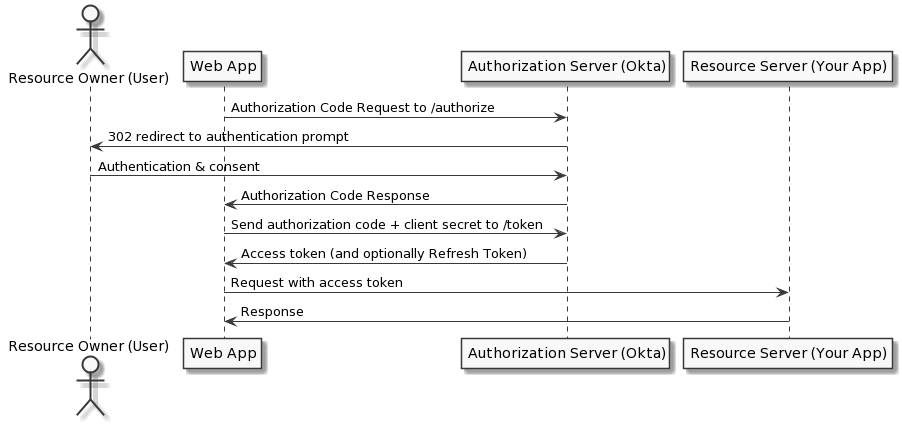
\includegraphics[width=1.0\textwidth]{gfx/oauth_auth_code_flow.png}
  \caption[Authorization Code Grant]{Authorization Code Grant \citep{okta:2020}}
  \label{fig:chapter02:oauth_auth_code_flow}
\end{figure}

In \autoref{fig:chapter02:oauth_auth_code_flow} ist der Authorization Code Grant Flow als Sequenzdiagramm abgebildet. Es ist zu sehen, dass es Beziehungen zwischen allen vier Rollen gibt, nämlich dem Ressource Owner, dem Client, in diesem Fall als „Web App“ gekennzeichnet, dem Authorization Server, Okta, und dem Ressource Server. 
In der Praxis ist der Ablauf folgendermaßen zu beschreiben:\smallskip

Ein Nutzer bedient eine Webapplikation (Client) und diese Webapplikation möchte, dass der Nutzer sie autorisiert, in ihrem Namen beispielsweise seine Adressdaten von dem Google-Konto abzufragen. In diesem Fall ist Google der Authorization und Ressource Server. Die Webapplikation, der Client, leitet den Nutzer auf den Google-Server weiter, wo er dann aufgefordert wird sich zu authentifizieren und der Webapplikation Erlaubnis zu erteilen, seine Adressdaten abzufragen. Daraufhin wird der Webbrowser des End-Nutzers zu dem Client zurückgeleitet und der Client erhält einen Token von dem Authorization Server, womit er die Ressource des End-Nutzers von dem Ressource Server abfragen kann. 

\section{JSON Web Token}
\label{sec:JSONWebToken}
Wenn ein Client einen Access Token von einem Authorization Server erhält, um Zugriff auf HTTP-Schnittstellen des Ressource Servers zu erhalten, sind diese Token bei den heutigen Implementierungen von Autorisationsservern sogenannte \ac{JSON} Web Token. Dies ist auch bei dem Autorisationsserver von Microsoft \citep{azuread:2021}, Azure Active Directory, sowie Keycloak \citep{keycloak:2021} der Fall. \ac{JSON} ist ein leichtgewichtiges Datenaustauschformat \citep{json:2006}.\smallskip

JSON Web Token ist eine Spezifikation für Token, die beschreibt wie die Tokens aufgebaut sind und welche Inhalte sie haben \citep{jwt:2015}.
Signierte JSON Web Token sind in drei Teile unterteilt: Header, Payload und die Signatur. Die Gesamtstruktur ist in JSON dargestellt, das heißt es gibt jeweils Schlüssel-Wert-Paare in JSON. Zur Übertragung werden die JSON Web Token base64-kodiert und hierbei werden jeweils die drei Teile, also Header, Payload und Signatur, durch einen Punkt (‚.‘) voneinander getrennt \citep{jwt:2015}. 
In dem Header und Payload stehen sogenannte Claims. Ein Claim ist ein Schlüssel-Wert-Paar. Diese liefern Informationen über den Token wie zum Beispiel der Claim „exp“, kurz für „Expiration Time“, der angibt, bis wann der Token gültig ist. Einen Token, der schon abgelaufen ist, sollte der Ressource Server nicht akzeptieren. Die Namen der Schlüssel der Claims sind standardisiert. 

\begin{lstlisting}[language=C++,frame=tb,caption={Beispiel JSON Web Token},label=lst:BeispielJSONWebToken]
  {
    alg: "RS256",
    typ: "JWT",
    kid: "KaD7XcL-5_0lEdjztl8fCqrR2R-uCf1BtCyngSfI7mg"
  }.
  {
    exp: 1625764809,
    iat: 1625763009,
    jti: "7df07f70-5c50-41fd-b757-2e3faa8c50e4",
    iss: "HTTP://localhost:9080/auth/realms/sample",
    aud: "account",
    sub: "de16edd9-a654-4769-b71c-3faf34583890",
    typ: "Bearer",
    azp: "test-app",
    session_state: "a19e1f5f-4080-488f-b193-a943925d62fc",
    acr: "1",
  }.
  [signature]   
\end{lstlisting}
\bigskip

Obenstehend ist ein rudimentärer dekodierter JSON Web Token dargestellt. In dem \autoref{subsec:OpenIDConnect:IDToken}
wird erläutert, welche Bedeutung die einzelnen Claims haben.

\subsection{JSON Web Token Signatur}
\label{sec:JSONWebToken:JSONWebTokenSignatur}

JSON Web Tokens sind in der Regel mit dem asymmetrischen Verfahren \ac{RSA} signiert \citep{jwt:2015}. Das bedeutet, dass mittels eines privaten Schlüssels, über den
nur der Ersteller des Tokens verfügt, also der Autorisationsserver, die Signatur erzeugt wird.
Daneben gibt es einen öffentlichen Schlüssel, mit dem die Signatur überprüft werden kann.
Das heißt es ist nicht möglich, dass der Client den Token verändern kann, da dann die
Signatur nicht mehr übereinstimmt.

\subsection{JSON Web Key}
\label{sec:JSONWebToken:JSONWebKey}
Im Falle eines durch RSA signierten JSON Web Token, ist der JSON Web Key der in JSON dargestellte öffentliche Schlüssel. Mithilfe dieses öffentlichen Schlüssels kann die Signatur aus dem Header und Payload des JSON Web Tokens berechnet werden. Entspricht die berechnete Signatur, der Signatur die in dem JSON Web Token vorhanden ist, ist der Token erfolgreich validiert und Integrität sowie Authentizität sind sichergestellt \citep{jwk:2015}.

\subsection{Base64 Kodierung}
\label{sec:JSONWebToken:Base64Kodierung}
JSON Web Token werden, wenn sie übertragen werden, in Base64 kodiert \citep{jwt:2015}. Base64 ist
keine Verschlüsselung und auch keine Datenkomprimierung, sondern dient vor allem dem
Zweck, dass Daten in ausschließlich ANSI-Zeichen kodiert übertragen werden. Irreguläre Zeichen wie Umlaute werden nicht übertragen \citep{base64:2006}. 

\section{OpenID Connect}
\label{sec:OpenIDConnect}
OpenID Connect ist eine Authentifizierungsschicht, die auf der OAuth2 Spezifikation
aufbaut. OpenID Connect baut auf OAuth2 eine Authentifizierung auf, indem es in dem JSON Web Token
Claims steckt, dass den Client, der den Token erhalten hat, nachdem sich ein End-Nutzer bei
dem Authorization Server authentifiziert hat, die Möglichkeit gibt die Identität dieses End-Nutzers zu verifizieren.
Diese Art von JSON Web Token, die der Client erhält, nennt sich ID Token \citep{openidconnect:2014}. 

\subsection{ID Token}
\label{subsec:OpenIDConnect:IDToken}
ID Token sind JSON Web Token, die gewisse Claims in ihrem Payload gesetzt haben \citep{openidconnect:2014}.

\begin{table}[H]
  \myfloatalign
  \begin{tabularx}{\textwidth}{|l|X|} \toprule
      \tableheadline{Claim} & \tableheadline{Beschreibung} \\ \midrule
      iss & Die Issuer-URL. Dies ist die URL des Authorization Server, der den Token 
      erstellt hat („Herausgeber“). \\
      \midrule
      sub & Das Subject. Dies ist ein eindeutiger Identifier des Nutzers, der sich 
      authentifiziert hat. \\
      \midrule
      aud & Die Audience. Das ist der Empfänger des Tokens, in der Regel die 
      Client-ID. \\
      \midrule
      exp & Expiration Time. Das ist der Zeitpunkt, zu dem der Token abgelaufen ist. \\
      \midrule
      iat & Issued at. Das ist der Zeitpunkt, zu dem der Token herausgegeben wurde. \\
      \bottomrule
  \end{tabularx}
  \caption[ID Token]{ID Token.}
  \label{tab:idtoken}

  \bigskip
In \autoref{tab:idtoken} sind die Claims zu sehen, die in dem Payload gesetzt sein müssen, damit ein
JSON Web Token als ID-Token bezeichnet werden kann.
\end{table}

\begin{table}[H]
  \myfloatalign
  \begin{tabularx}{\textwidth}{|l|l|X|} \toprule
      \tableheadline{Member} & \tableheadline{Type} & \tableheadline{Beschreibung} \\ \midrule
      sub & String & Die eindeutige ID des End-Nutzers.  \\
      \midrule
      name & String & Vor-und-Nachname.  \\
      \midrule
      given\_name & String & Vorname.  \\
      \midrule
      family\_name & String & Nachname.  \\
      \midrule
      nickname & String & Der Nickname. Das kann beispielsweise der Vorname sein.  \\
      \midrule
      email & String & Die E-Mail-Adresse.  \\
      \bottomrule
  \end{tabularx}
  \caption[Standard Claims]{Standard Claims.}
  \label{tab:standardclaims}
\end{table}

Zudem sind sogenannte Standard Claims spezifiziert, die Informationen über den 
authentifizierten End-Nutzer liefern und in den Payload eingetragen werden können \citep{openidconnect:2014}.  
Einige dieser Standard Claims sind in \autoref{tab:standardclaims} definiert. 

\subsection{Hybrid Flow}
\label{subsec:OpenIDConnect:HybridFlow}
Der Hybrid Flow ist der „Flow“ der beschreibt, wie der Client in OpenID Connect einen
Token erhalten kann. Es ist identisch mit dem Authorization Code Grant in OAuth2, nur 
dass hier neben einem Access Token der Client auch einen ID-Token von dem Authorization 
Server erhält. Der Hybrid Flow teilt sich in die folgenden acht Schritte auf \citep{openidconnect:2014}.

\begin{enumerate}
  \item Der Client bereitet eine Authorization Request vor. In dieser Request müssen folgende Daten hinterlegt sein:
    \begin{description}
      \item[response\_type:] In Falle des Authorization Code Grants muss hier code stehen. 
      \item[State:] Ein zufälliger String. 
      \item[Client\_Id:] Die ID des Clients. 
      \item[Scope:] Ein Wert, der den Geltungsbereich (scope) des Tokens angibt. 
      \item[Redirect\_uri:] Das ist die URI des Clients. An diese URI sendet der Autorisationsserver den Authorization Code. 
    \end{description}
  \item Der Client sendet die Authorization Request zu dem Authorization Server.
  \item Der Authorization Server authentifiziert den End-Nutzer. 
  \item Der Authorization Server holt sich die Autorisation/Einwilligung des End-Nutzers ein. 
  \item Der Authorization Server leitet den End-Nutzer zurück zu dem Client mit 
  einen Authorization Code.
  \item Der Client sendet eine Request mit dem Authorization Code an den Token-Endpunkt des Authorization Server, um Token zu erhalten. 
  \item Der Client erhält einen ID-Token und Access Token von dem Token-Endpunkt des Authorization Server.
  \item Der Client validiert den ID-Token und erhält den Subject Identifier des End-Nutzers.    
\end{enumerate}

\section{OAuth2 Endpunkte des Autorisationsservers}
\label{sec:OAuth2EndpunktedesAutorisationsservers}

Der Autorisationsserver ist über eine Reihe von Endpunkten für den Client und Ressource Server ansprechbar. Über den Token 
Endpunkt kann der Autorisationsserver beispielsweise Token an den anfragenden Client 
übermitteln. Im Folgenden werden die relevanten Endpunkte erläutert.

\subsection{Authorization Endpunkt}
\label{sec:OAuth2EndpunktedesAutorisationsservers:AuthorizationEndpunkt}
Dies ist der Endpunkt, an den der Client den End-Nutzer weiterleitet. Hier muss sich der 
End-Nutzer authentifizieren und gegebenenfalls den Client autorisieren, damit der Client einen Authorization Code erhält \citep{oauth2:2012}.

\subsection{Token Endpunkt}
\label{sec:OAuth2EndpunktedesAutorisationsservers:TokenEndpunkt}
Dies ist der Endpunkt des Autorisationsservers an den ein Client, falls er die notwendigen 
Informationen wie beispielsweise den Authorization Code besitzt, einen Token erhalten 
kann \citep{oauth2:2012}.

\subsection{JSON Web Key Set Endpunkt}
\label{sec:OAuth2EndpunktedesAutorisationsservers:JSONWebKeySet(JWKS)Endpunkt}
Dies ist der Endpunkt, in dem alle öffentlichen Schlüssel für die \ac{RSA}-Signatur des JSON Web 
Token abgefragt werden können [20]. Der Ressource Server nutzt diesen Endpunkt, um sich 
den passenden öffentlichen Schlüssel der Signatur des Tokens zu holen und damit die 
Signatur zu validieren und die Authentizität und Integrität des Tokens sicherzustellen \citep{jwk:2015}.

\section{Role Based Access Control}
\label{sec:Zugriffskontrolle:RoleBasedAccessControl(RBAC)}
\ac{RBAC}, zu Deutsch rollenbasierte Zugriffskontrolle, ist eine ANSI-NORM 
und sie beschreibt die Verknüpfung von Rollen, die Nutzern zugewiesen werden, mit 
Zugriffsprivilegien \citep{rbac:2006}. Sie ist eine Form der Zugriffskontrolle. Gemäß der Norm gibt es mehrere Definitionen:

\begin{description}
  \item[component:] Es gibt mehrere Komponenten in der ANSI-NORM, die beschreiben wie \ac{RBAC}
  umgesetzt werden kann.
  \item[objects:] Das ist das Objekt, auf das der Zugriff beschränkt werden soll. Das kann
  beispielsweise ein Datenbankeintrag, ein Drucker oder eine HTTP-Schnittstelle sein.
  \item[operations:] Eine Operation ist ein ausführbares Programm, was dem Nutzer Funktionen
  bereitstellt.
  \item[permissions:] Das ist die Zustimmung, eine Aktion auf eine durch \ac{RBAC} geschützte 
  Ressource durchzuführen.
  \item[Role:] Eine Rolle ist eine Jobfunktion innerhalb einer Organisation, die Autorität und 
  Verantwortlichkeiten eines Nutzers und der zugewiesenen Rolle assoziiert.
  \item[User:] Ein Nutzer ist definiert als eine Person, allerdings kann prinzipiell ein Nutzer auch ein 
  Objekt wie beispielsweise eine Maschine sein.
\end{description}

\section{Open Policy Agent}
\label{sec:OpenPolicyAgent}
Open Policy Agent (OPA) ist eine quelloffene Policy Engine, die Zugriffskontrolle von 
Applikationen entkoppelt \citep{opaperformance:2021:07}. Es entkoppelt das Treffen von Zugriffsentscheidungen von der Komponente, die Richtlinien durchsetzen muss.
Als Programmiersprache um diese Zugriffskontrolle zu definieren, wird Rego verwendet. 
Die Dateiendung von in Rego programmierten Zugriffsrichtlinien ist .rego.\smallskip

Im Wesentlichen werden dem OPA-Service Input-Daten in JSON zugesendet anhand dessen eine 
programmierte Zugriffskontrolle in Rego evaluiert, ob Zugriff gewährleistet werden darf und entsprechend sendet der OPA-Service an das anfragende Programm eine Zugriffsentscheidung. Dadurch das OPA als eigenständiger Service in einem Docker-Container ausgeführt wird und um die Zugriffskontrolle von Systemen mit Open Policy Agent zu entkoppeln, diese lediglich eine Unterstützung für HTTP und JSON mitbringen 
müssen, ist Open Policy Agent praktisch system und plattformunabhängig.

\begin{lstlisting}[language=C++,frame=tb,caption={Zugriffsrichtlinie in Rego},label=lst:ZugriffsrichtlinieinRego]
  package application.authz

  # Only owner can update the pet's information
  # Ownership information is provided as part of OPA's input
  default allow = false
  allow {
      input.method == "PUT"
      some petid
      input.path = ["pets", petid]
      input.user == input.owner
  }
\end{lstlisting}
\smallskip

In \autoref{lst:ZugriffsrichtlinieinRego} \citep{opaplayground:2021} ist eine solche Zugriffskontrolle in Rego programmiert. Diese Zugriffsrichtlinie ist wie folgt zu beschreiben:\smallskip

Falls eine HTTP-PUT-Anfrage auf den Pfad \emph{/pets/{petid}} eintrifft, muss der User dem 
Owner entsprechen. Anfragen, die nicht dem Pfad \emph{/pets/{petid}} entsprechen, werden abgelehnt. 

\begin{lstlisting}[language=C++,frame=tb,caption={Input-Daten für Open Policy Agent},label=lst:Input-DatenfürOpenPolicyAgent]
  {
    "method": "PUT",
    "owner": "bob@hooli.com",
    "path": [
        "pets",
        "pet113-987"
    ],
    "user": "alice@hooli.com"
  }
\end{lstlisting}
\smallskip

In \autoref{lst:Input-DatenfürOpenPolicyAgent} sind Input-Daten dargestellt. Wenn Open Policy Agent diese Input-Daten erhält, würde es eine negative Zugriffsentscheidung evaluieren. Die Zugriffsentscheidung ist in \autoref{lst:ZugriffsentscheidunginRego} zu sehen.

\begin{lstlisting}[language=C++,frame=tb,caption={Zugriffsentscheidung in Rego},label=lst:ZugriffsentscheidunginRego]
  {
    "allow": false
  }
\end{lstlisting}
\smallskip

Der Zugriff auf den Pfad /pets/pet113-987 kann nicht gegeben werden, da in \autoref{lst:Input-DatenfürOpenPolicyAgent} der owner nicht dem user entspricht. bob@hooli.com ist ungleich zu alice@hooli.com. 

\section{Apache Tomcat}
Apache Tomcat ist ein Webserver, der Spezifikationen der Java Enterprise Edition (EE) Plattform implementiert
\citep{tomcat:2021}. Dieser Webserver kann HTTP-Anfragen abhören und diese entgegennehmen und 
beantworten. Die für diese Arbeit relevanten Spezifikationen, die Tomcat implementiert, sind Jakarta Servlet, Servlet-Container
und Filter.

\begin{description}
  \item[Servlet:] Servlets interagieren mit Webclients über ein Anfrage/Antwort-Paradigma, das vom Servlet-Container implementiert wird \citep{servlet:2020}.
  \item[Servlet-Container:] Der Servlet-Container ist ein Teil eines Webservers oder Anwendungsservers, der die Netzwerkdienste bereitstellt
  über die Anfragen und Antworten gesendet werden. Ein Servlet-Container enthält und verwaltet auch Servlets während ihres Lebenszyklus \citep{servlet:2020}.
  \item[Filter:] Ein Filter ist ein wiederverwendbarer Code, der den Inhalt von HTTP-Anfragen, Antworten und Header-Informationen umwandeln kann. Filter erzeugen im Allgemeinen keine Antwort oder antworten auf eine Anfrage, wie es Servlets tun, sondern modifizieren oder passen die Anfragen für eine Ressource an und modifizieren oder passen Antworten von einer Ressource an \citep{servlet:2020}.
\end{description}

\section{Spring}
Spring ist ein quelloffenes Java-Framework, das die Implementierung von Anwendungen 
vereinfacht \citep{spring:2021}. Es teilt sich in eine Reihe von Teilprojekte auf. 

\subsection{Spring Boot}
Spring-Boot erleichtert die Implementierung mit dem Spring-Framework. In Spring-Boot Applikationen wird ein Apache Tomcat Webserver eingebettet \citep{springboot:2021}. Tomcat ermöglicht es dann, HTTP-Anfragen anzunehmen und diese durch Mappings in der Applikation zu beantworten.

\subsection{Spring Security}
Spring Security ist ein Teilprojekt des Spring-Frameworks. Spring Security bietet 
Unterstützung für OAuth2 und unter anderem auch für OAuth2 Ressource Server \citep{springsecurity:2021}. 
Mittels Spring Security ist es möglich einen OAuth2 Ressource Server zu implementieren, der 
Zugriff auf HTTP-Schnittstellen nur ermöglicht, wenn ein valider JSON Web Token in dem 
Authorization Header der HTTP-Anfrage gesendet wird. 

\section{Keycloak}
Keycloak ist eine Implementierung des Autorisationsserver und OpenID Provider der 
OAuth2 und OpenID Connect-Spezifikation. Das bedeutet, dass Clients von Keycloak Access 
Token sowie ID Token erhalten können.\smallskip

Daneben ist Keycloak auch ein Identity Provider, das heißt er ermöglicht es hinterlegten 
Nutzern sich zu authentifizieren. Damit ist der Authorization Code Grant und 
Hybrid Flow der OpenID Connect und OAuth2 Spezifikation möglich, denn es kann sich ein 
Nutzer authentifizieren, sodass dem Client ein Access Token und ID Token übermittelt 
werden kann \citep{keycloak:2021}.

\section{Apache JMeter und Metriken}
\label{sec:ApacheJMeterundMetriken}
Apache JMeter ist ein Programm, mit dem es unter anderem möglich ist die Schnittstellen eines HTTP-Servers auf 
Performance zu testen. Es kann Last auf den Server erzeugen und die Latenzen der Antworten des Servers sowie andere Metriken messen und protokollieren und diese Werte in Graphen visualisieren \citep{jmeter:2021}.
Da zum Testen der Performance verschiedene Metriken betrachtet werden, werden diese 
Metriken nachfolgend definiert. 

\begin{description}
  \item[Elapsed Time / Response Time:] Gemäß der Definition von Apache JMeter ist die Elapsed Time, auch Response Time 
  genannt, die Zeit von bevor dem Senden der HTTP-Anfrage an den Server bis nach dem 
  Eintreffen des in der Regel letzten Bytes der Antwort des Servers \citep{jmeterglossary:2021}. 
  \item[Latenz:] Gemäß der Definition von Apache JMeter ist die Latenz die Zeit von bevor dem Senden der 
  HTTP-Anfrage an den Server bis nach dem Eintreffen des in der Regel ersten Bytes der 
  Antwort des Servers \citep{jmeterglossary:2021}. 
  \item[Datendurchsatz:] Der Datendurchsatz (Throughput) wird berechnet aus dem Quotienten von Anzahl der Anfragen 
  und Zeiteinheit \citep{jmeterglossary:2021}. Es wird in dem Testplan selbst aus der ersten Anfrage bis zur letzten 
  Anfrage berechnet mit der folgenden Formel:

  \begin{equation}
    Datendurchsatz = \frac{Anzahl\;der\;Anfragen}{Gesamtzeit} 
  \end{equation}

  \item[Connect Time:] Die Connect Time ist die Zeit, die in Anspruch genommen wird, eine Verbindung mit dem 
  Server aufzunehmen \citep{jmeterglossary:2021}. Im Falle von der Nutzung von \ac{TCP} ist das der Three-Way-Handshake. TCP ist ein verbindungsorientiertes Protokoll \citep{tcp:1981}.
\end{description}

\section{Application Performance Index}
Der Application Performance Index (Apdex) ist ein offener Standard, der die Nutzerzufriedenheit 
hinsichtlich der Response Time in Webapplikationen berechnet \citep{apdex:2007}. Es wird ein Wert T 
festgelegt, der die Response Time angibt, bis zu der der Nutzer zufrieden ist. Dann gibt es 
einen zweiten Wert, der ein Vielfaches von T ist und angibt, bis zu welcher Länge der 
Response Time der Nutzer Antwortzeiten toleriert. Bei allen Werten darüber ist der Nutzer 
frustriert. Aus diesen Werten errechnet sich ein Ergebnis für den Application 
Performance Index, wobei hier 1.0 der beste Wert ist, das heißt der Nutzer ist vollständig 
zufrieden.\smallskip

\begin{table}[h]
  \myfloatalign
  \begin{tabularx}{\textwidth}{|l|l|X|} \toprule
      \tableheadline{Level} & \tableheadline{Multiplier} & \tableheadline{Time T} \\ \midrule
      Zufrieden & <= T & <= 1,2 Sekunden  \\
      \midrule
      Toleriert & >T, <= 4T & [1,2 Sekunden, 4,8 Sekunden]  \\
      \midrule
      Frustriert & > 4T & > 4,8 Sekunden  \\
      \bottomrule
  \end{tabularx}
  \caption[Beispiel von Grenzwerten eines Application Performance Index]{Beispiel von Grenzwerten eines Application Performance Index.}
  \label{tab:ApplicationPerformanceIndex}
\end{table}

In \autoref{tab:ApplicationPerformanceIndex} sind beispielhaft Grenzwerte für einen Application Performance Index dargestellt. Wenn die durchschnittliche Response Time <= 1,2 Sekunden beträgt, ist der Nutzer vollständig zufrieden. Response Times zwischen 1,2 und 4,8 Sekunden toleriert der Nutzer 
und bei Response Times größer als 4,8 Sekunden ist der Nutzer frustriert. Am Beispiel 
Webanwendungen wäre hier die Response Time die Zeit von bevor dem Senden einer Anfrage für eine HTTP-Schnittstelle, beispielsweise die GET-Anfrage, um eine Webseite darzustellen, bis zum Erreichen des letzten Bytes der Antwort des Servers, d.h. bis die Webseite bei dem Nutzer vollständig dargestellt ist.\smallskip 

Aus den durchschnittlichen Response Times und den festgelegten Werten T, errechnet sich der Application Performance Index.

\begin{equation}
  Apdex_T = \frac{Satisfied\;count + \frac{Tolerating\;count}{2}}{Total\;samples}
\end{equation}

In der obenstehenden Gleichung ist die Formel zur Berechnung des Application Performance Index dargestellt \citep{apdex:2007}. Satisfied count ist hierbei die Anzahl der Anfragen deren Beantwortung <= T dauerten und der Tolerating 
count diejenigen Anfragen die <= 4T dauerten, wobei diese nur eine halbe Gewichtung 
haben. Die Summe aus beiden Werten wird durch die Anzahl aller Anfragen geteilt. Wenn die Response Times aller Anfragen <= T betrugen, errechnet sich ein perfekter Index, 
der 1,0 beträgt.

\section{Postman}
Postman ist ein API-Client, mit dem unter anderem HTTP-Anfragen gesendet und Antworten 
des Servers erhalten werden können. Außerdem bietet Postman Unterstützung für 
OAuth2 an, das heißt es ist mittels Postman möglich, den Authorization Code Grant und
Hybrid Flow abzuhandeln, um dadurch Token von einem Authorization Server zu erhalten. Hierbei ist Postman der Client der OAuth2 Spezifikation \citep{postman:2021}.

\section{Docker-Container}
Ein Docker-Container ist ein leichtes, eigenständiges, ausführbares Softwarepaket, das alles enthält, was zum Ausführen einer Anwendung erforderlich ist: Code, Laufzeit, Systemtools, Systembibliotheken und Einstellungen. \citep{docker:2021}. 

\section{Kubernetes}
Kubernetes ist eine Plattform zur Verwaltung von Container-Anwendungen. Es ermöglicht die Konfiguration von Container-Anwendungen sowie die Automatisierung der Bereitstellung von Container-Anwendungen. Außerdem bietet Kubernetes Funktionen zur Bereitstellung, Skalierung, Lastausgleich, Protokollierung und Überwachung der Container-Anwendungen \citep{kubernetes:2020}. Mit Container-Anwendungen sind in diesem Fall Docker-Container gemeint, in denen Anwendungen ausgeführt werden. Kubernetes wurde von Google 2014 als Open-Source Projekt zur Verfügung gestellt. Es gibt eine Reihe von Komponenten in Kubernetes, die nachfolgend definiert werden.  

\begin{description}
  \item[Node] Ein Node ist ein physischer Computer oder virtuelle Maschine, der als Arbeitsmaschine in einem Kubernetes Cluster dient. Auf einem Node werden Container-Anwendungen ausgeführt \citep{kubernetesclusternode:2019}. 
  \item[Cluster] In einem Cluster können sich mehrere Nodes befinden. Kubernetes koordiniert in einem Cluster Nodes, die miteinander verbunden sind, um als eine Einheit zu arbeiten \citep{kubernetesclusternode:2019}.
  \item[Pod] Ein Pod ist die kleinste Einheit, die in Kubernetes erstellt und verwaltet werden kann. In einem Pod laufen ein oder mehrere Docker-Container, die sich Speicher- und Netzwerkressourcen teilen \citep{kubernetespods:2021}.  
  \item[Deployment] Ein Deployment weist an, wie Instanzen einer Anwendung erstellt und aktualisiert werden. Hierzu wird eine Deployment Konfiguration geschrieben und auf ein Kubernetes Cluster angewandt, woraufhin Kubernetes ein Pod erstellt. Darüber hinaus bietet Kubernetes für Deployments Selbstheilungsmechanismen. Wenn beispielsweise ein Node, der eine Instanz einer Applikation hostet, ausfällt, ersetzt der sogenannte Deployment Controller diese Instanz durch eine Instanz auf einem anderen Node im Cluster \citep{kubernetesdeployment:2021}.
  \item[Service] Ein Service definiert Richtlinien wie auf Pods zugegriffen werden können. Es regelt also, wie ein Nutzer auf einen Pod in einem Cluster von außerhalb des Clusters zugreifen kann, als auch wie Pods miteinander innerhalb des Clusters kommunizieren können. Hierfür muss ebenfalls eine Konfiguration geschrieben werden \citep{kubernetesservice:2021}. 
\end{description}

\begin{figure}[!htb]
  \centering
  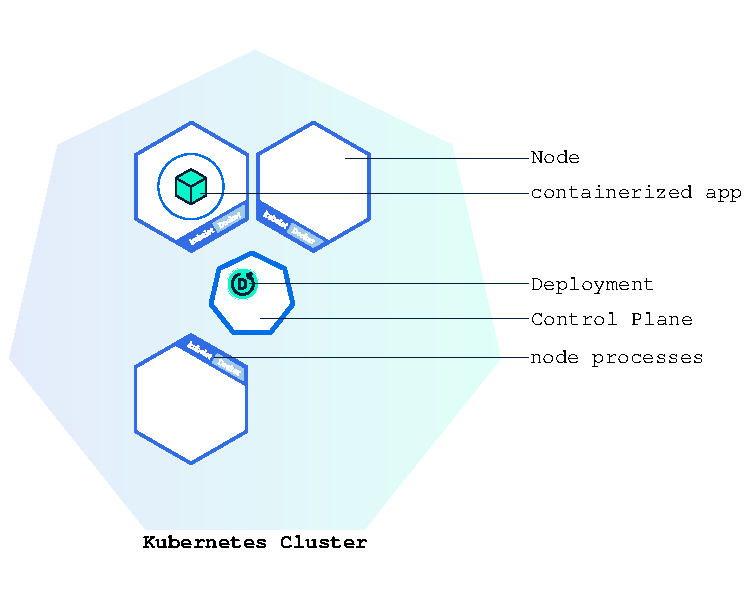
\includegraphics[width=1.0\textwidth]{gfx/module_02_first_app.pdf}
  \caption[Kubernetes Cluster]{Kubernetes Cluster \citep{kubernetesdeployment:2021}}
  \label{fig:chapter02:KubernetesCluster}
\end{figure}

In \autoref{fig:chapter02:KubernetesCluster} ist ein Kubernetes Cluster mit drei Nodes beispielhaft dargestellt. In einem Node ist zu sehen, dass dort eine kontainerisierte Anwendung läuft, die ein Docker-Container ist. Auf jedem Node im Cluster wird kubelet ausgeführt, der ein Agent ist und sicherstellt, dass Container in einem Pod ausgeführt werden. Um mit dem Cluster zu kommunizieren, um beispielsweise Pods zu starten, gibt es die Kubernetes-API und kubectl als Kommandozeilenprogramm \citep{kuberneteskubelet:2020}. 

\section{Zusammenfassung der technischen Grundlagen}
Es wurden die nötigen technischen Grundlagen zusammengetragen. Was im nachfolgenden Kapitel folgt ist die Systemarchitektur.
Beide Systeme sind OAuth2 Ressource Server, die Spring-Boot Webapplikationen sind und mit Spring-Security ihre HTTP-Schnittstellen sichern. Das bedeutet, dass diese Schnittstellen erwarten, dass ein valider JSON Web Token in dem Authorization Header der HTTP-Anfrage mitgesendet wird. Dieser JSON Web Token wird durch Keycloak ausgestellt, in OAuth2-Vokabular ist dies der Authorization Server. In OpenID Connect Vokabular würde bei Keycloak von einem OpenID Provider gesprochen werden. In dem ID Token, der von dem 
Authorization Server übermittelt wird, werden Attribute des Nutzers in den Payload 
gemappt, unter anderem auch die Rollenzugehörigkeit. Die Spring-Boot Applikationen 
validieren den Token jeweils, in dem sie die Signatur des Tokens überprüfen. Dies 
geschieht, indem der öffentliche Schlüssel über den JSON Web Key Set Endpunkt des Authorization 
Server geholt und damit aus dem Header und Payload die Signatur berechnet und auf 
Gleichheit überprüft wird. Bei Erfolg 
entspricht dies einer Authentifizierung des Nutzers.\smallskip

Beide Ressource Server haben als Zugriffskontrolle \ac{RBAC} 
implementiert, das heißt in dem Token muss die Rolle \emph{ROLE\_USER} vorhanden sein, damit 
Zugriff auf die HTTP-Schnittstelle erfolgen kann. Allerdings wird dies in beiden Servern auf 
unterschiedliche Weise realisiert. In dem einen Server wurde die Zugriffskontrolle in dem Server 
selbst implementiert, in dem anderen Server wird diese entkoppelt durch den Open Policy Agent. 
Dieser wird als eigenständiges Programm in einem Docker-Container ausgeführt und die 
Kommunikation zwischen Ressource Server und OPA-Service geschieht auf localhost-zu-localhost Basis. 
Um die Performance zu testen, wird Apache JMeter verwendet. JMeter erzeugt Last auf die 
beiden Servern, das heißt es sendet HTTP-Anfragen mit validem Token an die Ressource 
Server und misst die Latenzen der Antworten. Neben der Latenz wird auch die Response 
Time und Connect Time gemessen und der Datendurchsatz berechnet. Außerdem werden während aller Tests die CPU-Auslastung und Arbeitsspeicherbelegung betrachtet.\smallskip

Zudem wird das System mit entkoppelter Zugriffskontrolle als drittes Testsystem auch in ein Kubernetes Cluster deployed und verglichen inwiefern sich eine Nutzung von Kubernetes auf die Performance auswirkt. 
\chapter{Einfluss von externer Zugriffskontrolle auf die Performanz in OAuth2 Systemen}
\label{sec:Einfluss von externer Zugriffskontrolle auf die Performanz in OAuth2 Systemen}

Zunächst werden alle Komponenten des Systems beschrieben. Da es sich um ein OAuth2-
System handelt, gibt es alle Rollen, die auch im \autoref{subsec:OAuth2:RolleninOAuth2} beschrieben 
wurden. Also Authorization Server, Ressource Server, Client und End-Nutzer. 

\section{Keycloak als Authorization Server und Identity Provider}
\label{sec:KeycloakalsAuthorizationServerundIdentityProvider}

Keycloak ist eine Implementierung des Authorization Server der OAuth2 und OpenID 
Connect Spezifikation. Das bedeutet, dass Keycloak unter anderem dafür zuständig ist, den 
Clients Access und ID Token durch den Hybrid Flow zuzusenden. 
Keycloak wurde in der Version 12.0.4 genutzt, und in einem Docker-Container ausgeführt. 
Die genutzte Konfiguration ist in den Anlagen vorzufinden. 
Die Tokens, die Keycloak herausgibt, sind JSON Web Token und mit RSA asymmetrisch 
signiert. Konkret sind sie mit RS256 signiert, das heißt die Schlüssel sind 256 Bit groß.\smallskip

Neben einem Authorization Server ist Keycloak auch ein sogenannter Identity Provider. Das 
bedeutet, dass in Keycloak Nutzer angelegt werden können und diese Nutzer auch 
verwaltet werden können. 
Damit sich Nutzer bei Keycloak authentifizieren können, musste zunächst ein Nutzer in 
Keycloak angelegt werden. Dies ist wichtig, damit dem Client überhaupt ein Token 
ausgestellt werden kann durch den Hybrid Flow und damit die Attribute des Nutzers in den 
Token gemappt werden, denn anhand dieser Attribute wird dann ja im Ressource Server 
die Zugriffe auf dessen HTTP-Schnittstelle kontrolliert. Die Charakterisierung des Nutzers ist 
an dieser Stelle wichtig, da die vorhandenen Attribute, die den Nutzern zugewiesen werden, auch 
in den Token gemappt werden und die Größe des Tokens Einfluss auf die Performance 
hat.

\begin{figure}[htbp]
  \centering
  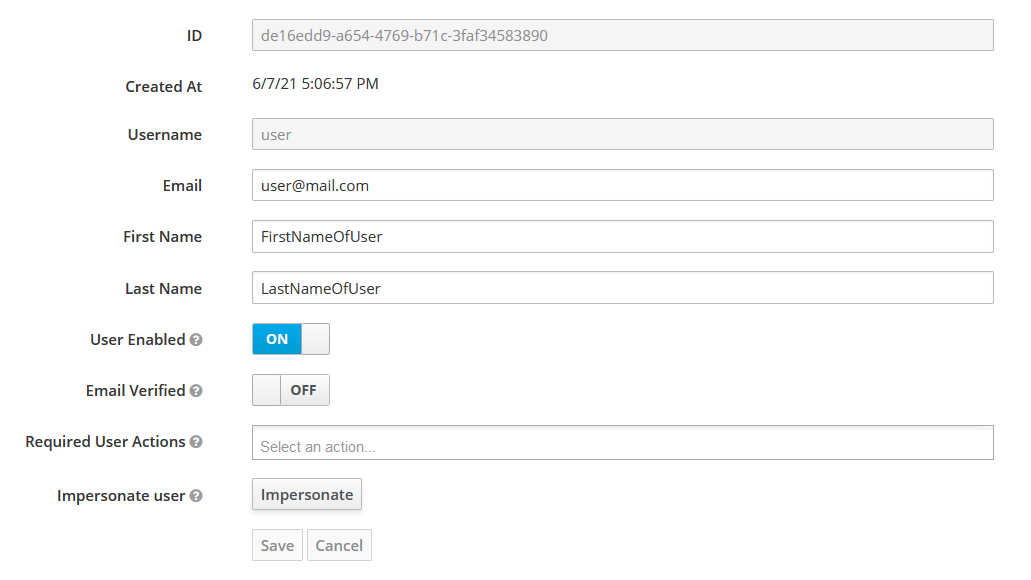
\includegraphics[width=1.0\textwidth]{gfx/keycloak-sample-user.PNG}
  \caption{Keycloak Sample User}
  \label{fig:chapter03:keycloak-sample-user}
\end{figure}

In \autoref{fig:chapter03:keycloak-sample-user} Keycloak Sample User ist der erstellte Nutzer in Keycloak zu sehen. Neben 
den Standardattributen wird dem Nutzer auch eine Rolle zugewiesen, und zwar die Rolle ROLE\_USER.\bigskip

\begin{figure}[htbp]
  \centering
  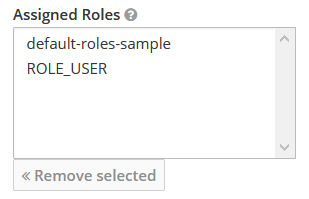
\includegraphics[width=0.5\textwidth]{gfx/keycloak-sample-user-role.PNG}
  \caption{Keycloak Sample User Role}
  \label{fig:chapter03:keycloak-sample-user-role}
\end{figure}

Dies ist in Keycloak möglich und damit lässt sich in den Applikationen dann eine 
rollenbasierte Zugriffskontrolle realisieren. In \autoref{fig:chapter03:keycloak-sample-user-role} sind die zugewiesenen Rollen zu sehen. default-roles-sample ist eine durch Keycloak automatisch 
zugewiesene Rolle und hat hier keine weitere Relevanz. 
Außerdem wurde diesem Nutzer noch eine Gruppenzugehörigkeit und ein weiteres Attribut 
hinzugewiesen. Gruppenzugehörigkeiten sind in Firmen oftmals die Bürostandorte, 
Abteilungen und dergleichen. Nach Gruppenzugehörigkeiten wird in der Regel nicht 
autorisiert, denn dafür sind Rollen zuständig. Die Gruppenzugehörigkeit und das weitere 
Sample-Attribut hat hier nur den Sinn, dass es den Token umfangreicher macht und dies 
dient dazu, realistische Testbedingungen zu schaffen. Der Nutzer ist also in der Gruppe 
Users und hat als zusätzliches Attribut das statische Schlüssel-Wert-Paar Attribute1:UserAttribute1. 
Zusätzlich musste in Keycloak ein Client registriert werden. Der Client ist diejenige 
Komponente im OAuth2 System, die den Token von dem Authorization Server, also 
Keycloak, erhält und den Token nutzt, um Zugriff auf Schnittstellen des Ressource Servers 
zu erhalten. Für den Hybrid Flow ist mindestens eine Client-ID notwendig. In 
diesem Fall wurde ein sogenannten confidential client in Keycloak registriert. Dieser muss 
sich mit seinen Daten, also Client-ID und Client Secret, bei Keycloak authentifizieren, um 
Token zu erhalten.

\section{Erhalt eines Tokens mit Postman}
Um Token durch den Hybrid Flow zu erhalten, wird ein Client und ein Nutzer benötigt, der 
sich für den Client authentifiziert und den Authorization Server, der den Token ausstellt. 
Der erstellte Nutzer wurde im vorhergehenden Kapitel in Keycloak, dem Authorization 
Server, gezeigt. Der Nutzer muss einen Browser Agenten bedienen, damit der Client über 
den Hybrid Flow Token erhalten kann. Als Client wurde der API-Client Postman verwendet, 
der eingebauten Support für OAuth2 besitzt und mittels eines Browsers den Hybrid Flow 
ausführen und damit Postman, also der Client, Token erhalten kann. 

\begin{figure}[htbp]
  \centering
  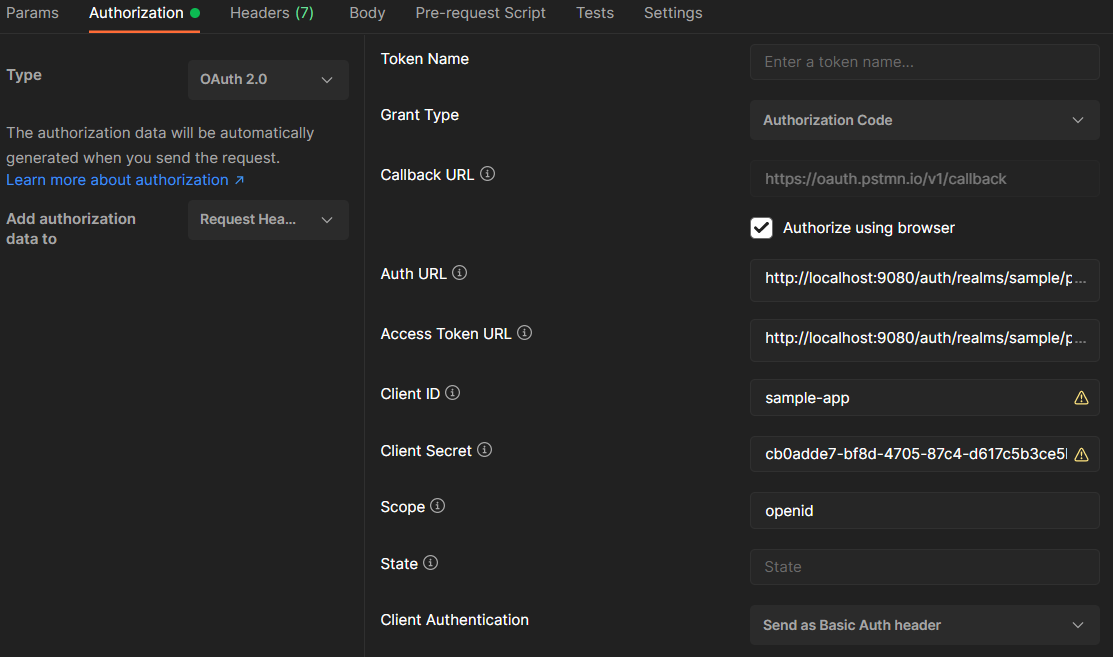
\includegraphics[width=1.0\textwidth]{gfx/postman-get-token3.PNG}
  \caption{Authorization Code Grant mit Postman}
  \label{fig:chapter03:postman-get-token3}
 \end{figure}

In \autoref{fig:chapter03:postman-get-token3} ist das Menü in Postman zu sehen. Um einen Token in Postman mit dem 
eingebauten OAuth2 Support von Postman zu erhalten, mussten einige Daten angegeben
werden, damit Postman den Authorization Code Grant beziehungsweise Hybrid Flow 
ausführen kann. 
Wie in \autoref{subsec:OAuth2:ErhaltvonToken} beschrieben, gibt es mehrere Wege wie ein Client einen Token 
erhalten kann. Hier musste als Grant Type Authorization Code angegeben werden. 
Dann musste die Auth URL, also der Authorization Endpunkt des Authorization Server 
angeben werden. Hier wird der Browser des End-Nutzers hingeleitet, wo sich dann der End-Nutzer authentifizieren muss. 
Die Access Token URL ist diejenige URL, von der Postman in Austausch von einem 
Authorization Code einen Token erhalten kann. Den Authorization Code erhält Postman, 
nachdem sich der End-Nutzer bei Keycloak authentifiziert hat. 
Diese Endpunkte sind in Keycloak in der Admin-Konsole unter Real Settings vorzufinden. 
Als Client ID und Client Secret wurden die Werte eingetragen, die bei der Registrierung des 
Clients im vorherigen Kapitel erhalten wurden. 
Als Scope wurde openid angegeben, damit die notwendigen Nutzerattribute von dem End-Nutzer, der sich bei Keycloak authentifiziert in den ID Token gemappt werden, da diese 
Attribute ja benötigt werden, um eine Zugriffskontrolle zu realisieren. 
Wenn diese Anfrage in Postman abgeschickt wurde, öffnet sich der Browser und man 
erreicht die Auth-URL von Keycloak, in der aufgefordert wird, dass sich der End-Nutzer 
authentifiziert. Hier muss sich nun der End-Nutzer authentifizieren, der in Keycloak als Authorization Server 
und Identity Provider erstellt wurde. Die Auth URL ist nachfolgend dargestellt. 

\begin{lstlisting}[language=C++,frame=tb,caption={Authorization Request},label=lst:AuthorizationRequest]
  HTTP://localhost:9080/auth/realms/sample/protocol/openid-connect/auth?
  response_type=code
  &state=
  &client_id=sample-app
  &scope=openid
  &redirect_uri=HTTPs%3A%2F%2Foauth.pstmn.io%2Fv1%2Fcallback
\end{lstlisting}
\bigskip

In \autoref{lst:AuthorizationRequest} ist die HTTP-POST-Request dargestellt, mit der dann Postman, nachdem sich der End-Nutzer 
authentifiziert hat, einen Authorization Code erhält, den Postman dann durch einen Token 
von Keycloak austauschen kann. Die Paramater, die hier an Keycloak übertragen werden, 
sind diejenigen, die auch in \autoref{subsec:OAuth2:ErhaltvonToken} beschrieben sind, nämlich:

\begin{itemize}
  \item Response\_type
  \item State
  \item Client\_Id
  \item Scope
  \item Redirect\_uri
\end{itemize}

Nachdem sich nun der End-Nutzer authentifiziert hat, erhält Postman einen JSON Web Token. Die 
Token-Anfrage, bei der der Authorization Code durch einen Token ausgetauscht wird, 
geschieht automatisch und wird hier nicht beschrieben.

\begin{lstlisting}[frame=tb,caption={Base64-kodierter JSON Web Token},label=lst:Base64-kodierterJSONWebToken]
  eyJhbGciOiJSUzI1NiIsInR5cCIgOiAiSldUIiwia2lkIiA6ICJhUV83TjRENmN5MEVnVnVlR2ZrSWRobG5Ud1FoYi1IVDJlM21wWWFHV0o4In0.

  eyJleHAiOjE2MjY2NDE0MzQsImlhdCI6MTYyNjYzOTYzNCwiYXV0aF90aW1lIjoxNjI2NjM5NjMzLCJqdGkiOiJiZjA3MDQwNS03NDY5LTQ1NTQtOWViOC1mNTcwMjNhMGY0ZDMiLCJpc3MiOiJodHRwOi8vbG9jYWxob3N0OjkwODAvYXV0aC9yZWFsbXMvc2FtcGxlIiwiYXVkIjoiYWNjb3VudCIsInN1YiI6ImJmNDlmODdmLTY2ZDktNDNjZS1hNzRmLTgyMzNkY2ZmODNhYiIsInR5cCI6IkJlYXJlciIsImF6cCI6InNhbXBsZS1hcHAiLCJzZXNzaW9uX3N0YXRlIjoiNzFiMzJhZjgtNTQ0OS00OTMzLWJlZmUtZDQzODAwNzdkYzI1IiwiYWNyIjoiMSIsInJlYWxtX2FjY2VzcyI6eyJyb2xlcyI6WyJkZWZhdWx0LXJvbGVzLXNhbXBsZSIsIlJPTEVfVVNFUiIsIm9mZmxpbmVfYWNjZXNzIiwidW1hX2F1dGhvcml6YXRpb24iXX0sInJlc291cmNlX2FjY2VzcyI6eyJhY2NvdW50Ijp7InJvbGVzIjpbIm1hbmFnZS1hY2NvdW50IiwibWFuYWdlLWFjY291bnQtbGlua3MiLCJ2aWV3LXByb2ZpbGUiXX19LCJzY29wZSI6Im9wZW5pZCBlbWFpbCBwcm9maWxlIiwiZW1haWxfdmVyaWZpZWQiOmZhbHNlLCJyb2xlcyI6WyJkZWZhdWx0LXJvbGVzLXNhbXBsZSIsIlJPTEVfVVNFUiIsIm9mZmxpbmVfYWNjZXNzIiwidW1hX2F1dGhvcml6YXRpb24iXSwibmFtZSI6IkZpcnN0TmFtZU9mVXNlciBMYXN0TmFtZU9mVXNlciIsImF0dHJpYnV0ZTEiOiJVc2VyQXR0cmlidXRlMSIsImdyb3VwcyI6WyIvVXNlcnMiXSwicHJlZmVycmVkX3VzZXJuYW1lIjoidXNlciIsImdpdmVuX25hbWUiOiJGaXJzdE5hbWVPZlVzZXIiLCJmYW1pbHlfbmFtZSI6Ikxhc3ROYW1lT2ZVc2VyIiwiZW1haWwiOiJ1c2VyQG1haWwuY29tIn0.

  b9BWNcf6ZaG-3sgX86YLu58vyk-HiZkDbLEdp5PgHEuZ6Q9omqjRsZCv4poQZtiqWrHSbprjiwfLadfPwz8sK9UOCrDs2KGd9Ev1nZrnI8JbhS3yfixkKTDyOOCja6KGAoYzfAnc4UVwfgP7xevBrWAnbpWGfVSStAPWBSlk0ICCHw8Kwkrly95tggsZLpuKFi7Mr0wrKlbB9-KjKYSoQhvZ6pQCFFJ83SjZ-sj_v7tkHXX79wf-exIgy2k64JBXViT66JKg9t33wnFEHtnnLG-nvoqGirPeRTZT0T_skmHNTg-p9zIxN3uYPMfKJ0o1yRUjvDD4LG1WYWKUahu82Q
\end{lstlisting}
\bigskip

In \autoref{lst:Base64-kodierterJSONWebToken} ist der Base64 kodierte Token zu sehen. Wie man sieht, ist er in drei Teile 
unterteilt: Dem Header, dem Payload und der Signatur. Um ihn zu dekodieren und den 
Inhalt in JSON betrachten zu können, gibt es Dienste, die das Übernehmen. Auf \url{https://jwt.io/} ist es möglich, Base64 kodierte JSON Web Token zu dekodieren. 

\begin{lstlisting}[frame=tb,caption={Dekodierter JSON Web Token},label=lst:DekodierterJSONWebToken]
{
    "alg": "RS256",
    "typ": "JWT",
    "kid": "ht0BHd8h1Q_CPuOLMj2TjiBJd6ukIROuxFmimbECbsk"
}.
{
    "exp": 1626691594,
    "iat": 1626689794,
    "auth_time": 1626689528,
    "jti": "dacddb77-6de4-4464-b623-b766a8624cda",
    "iss": "HTTP://localhost:9080/auth/realms/sample",
    "aud": "account",
    "sub": "8cf89140-e8d6-4850-b416-3cceda982ec2",
    "typ": "Bearer",
    "azp": "sample-app",
    "session_state": "c8e12b53-1203-4d8e-a27c-ea54f3f86d60",
    "acr": "0",
    "realm_access": {
      "roles": [
        "default-roles-sample",
        "ROLE_USER",
        "offline_access",
        "uma_authorization"
      ]
    },
    "resource_access": {
      "account": {
        "roles": [
          "manage-account",
          "manage-account-links",
          "view-profile"
        ]
      }
    },
    "scope": "openid email profile",
    "email_verified": false,
    "roles": [
      "default-roles-sample",
      "ROLE_USER",
      "offline_access",
      "uma_authorization"
    ],
    "name": "FirstNameOfUser LastNameOfUser",
    "attribute1": "UserAttribute1",
    "groups": [
      "/Users"
    ],
    "preferred_username": "user",
    "given_name": "FirstNameOfUser",
    "family_name": "LastNameOfUser",
    "email": "user@mail.com"
}.
[Signature]
\end{lstlisting}
\bigskip

In \autoref{lst:DekodierterJSONWebToken} ist der dekodierte JSON Web Token dargestellt, den Keycloak erstellt und an Postman gesendet hat, nachdem sich der End-Nutzer der in \autoref{sec:KeycloakalsAuthorizationServerundIdentityProvider} erstellt wurde, authentifiziert hat. Wie zu sehen ist, sind die Nutzerattribute, also die Standardclaims, in diesen Token gemappt. Das heißt der Vor-und-Nachname, die E-Mail-Adresse, der Nickname sowie das Claim sub. 
Zudem ist die Gruppenzugehörigkeit zu sehen, denn User ist ja in der Gruppe Users. Außerdem ist unter dem Schlüssel roles auch die Rolle ROLE\_USER vorzufinden. Diese Rolle wurde dem End-Nutzer in Keycloak zugewiesen und nach dieser Rolle wird dann bei der Schnittstelle im Ressource Server die Zugriffe kontrolliert, das heißt in dem Token muss diese Rolle gemappt sein, ansonsten sollte kein Zugriff erlaubt werden. Die restlichen Rollen, die in diesem Token zu sehen sind wie beispielsweise default-roles-sample, wurden automatisch von Keycloak erstellt und werden hier nicht weiter erläutert.\smallskip

Außerdem sind die Claims vorzufinden, die in einem ID Token Pflicht sind wie beispielsweise exp, der angibt, wann der Token abläuft. Erklärungen zu diesen Claims sind in \autoref{subsec:OpenIDConnect:IDToken} zu finden. Diese werden hier nicht weiter erläutert. 
Im Header ist unter anderem das Claim alg: RS256 vorzufinden, das angibt, dass der Token durch RSA mit 256 Bit großen Schlüssel asymmetrisch signiert ist. Was hierbei wichtig ist, dass durch diese Signatur, die in \autoref{lst:DekodierterJSONWebToken} lediglich aus Platzgründen mit [Signature] gekennzeichnet ist, die Authentizität und Integrität des Tokens sichergestellt ist. Der Ressource Sever kann sich den passenden öffentlichen Schlüssel von Keycloak holen und damit dann die Authentizität und Integrität des Tokens validieren. 
Nun wurde also durch den Authorization Code Grant ein Token von dem Authorization Server Keycloak erhalten mit dem es möglich ist, auf die HTTP-Schnittstellen eines Ressource Servers zuzugreifen. Diese Ressource Server werden im nachfolgenden Kapitel beschrieben. 

\section{Ressource Server}
Beide Ressource Server sind in Java mithilfe des Spring-Frameworks implementiert. Die Ressource Server sind Spring-Boot Anwendungen, das bedeutet, dass ein Apache Tomcat Webserver in der Applikation eingebettet ist und automatisch gestartet wird. Die Ressource Server können also HTTP-Anfragen von Clients entgegennehmen und diese beantworten.\smallskip

Die verwendete Spring-Boot Version ist 2.4.8 mit Apache Tomcat 9.0.48, welcher über den Port 8080 erreichbar ist. Alle Versionen der verwendeten Technologien wie die Datenbank und der Object-Relational Mapper Hibernate können aus der Spring-Boot Version hergeleitet werden und werden deshalb im weiteren Verlauf nicht genannt. Als Java Runtime Envinroment (JRE) wurde Version 11 verwendet.\smallskip

Gemäß der OAuth2 Spezifikation bezeichnet man diese Server Ressource Server, weil sie valide Tokens erwarten, die von einem Authorization Server ausgestellt werden, damit sie den Clients Zugriff auf ihre Schnittstellen geben können. Im weiteren Verlauf werden beide Ressource Server auf ihre Performance getestet. Der einzige Unterschied zwischen beiden Servern besteht darin, wie sie Zugriffsentscheidungen evaluieren, das heißt wie sie ermitteln, ob der Client berechtigt ist auf die Schnittstelle des Servers zuzugreifen. Dies wird als Zugriffskontrolle bezeichnet. Der eine Ressource Server implementiert diese Zugriffskontrolle in der Spring-Boot Applikation selbst, während der andere diese entkoppelt mit Open Policy Agent, das ein externes Programm ist und per HTTP für den Server erreichbar ist, um eine Zugriffsentscheidung zu erhalten.\smallskip

Zu erwähnen ist, dass eine Implementierung von Ressource Servern grundsätzlich in jeder Programmiersprache erfolgen kann, die HTTP-, JSON-, Base64-Kodierung-sowie-RSA unterstützt. 

\subsection{Schnittstelle}
\label{subsec:Schnittstelle}
Beide Ressource Server haben eine HTTP-GET-Schnittstelle implementiert, welche Daten aus einer SQL-Datenbank holt und sie dem anfragenden Client sendet. Dies ist genau die Schnittstelle, die nicht für alle frei zugänglich ist, sondern nur Nutzern zur Verfügung steht, die einen validen JSON Web Token haben und der Rolle ROLE\_USER zugehörig sind. 

\begin{lstlisting}[language=Java,frame=tb,caption={HTTP-Schnittstelle der Ressource Server},label=lst:HTTP-Schnittstelleder Server]
  /**
  * {@code GET  /documents} : get all the documents.
  *
  * @return the {@link ResponseEntity} with status {@code 200 (OK)} 
  * and the list of documents in body.
  */
  @GetMapping("/documents")
  public List<Document> getAllDocuments() {
     log.debug("REST request to get all Documents");
     return documentService.findAll();
  }
\end{lstlisting}
\bigskip

In \autoref{lst:HTTP-Schnittstelleder Server} ist diese Schnittstelle dargestellt. Sie wird auf „/documents“ gemappt, das bedeutet, dass falls der Ressource Server auf dem localhost gestartet wird, und der Client sich ebenso auf dem localhost befindet, er diese Schnittstelle über den Pfad „localhost:8080/documents“ ansprechen kann. 8080 ist hierbei der Port, auf dem Apache Tomcat HTTP-Anfragen abhört.
Diese Schnittstelle wurde in eine für Spring-Anwendungen typischen objektorientierten Architektur implementiert.

\begin{figure}[htbp]
  \centering
  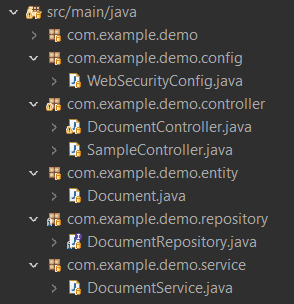
\includegraphics[width=0.5\textwidth]{gfx/projekstruktur-spring.png}
  \caption{Projekstruktur Spring Applikation}
  \label{fig:chapter03:projekstruktur-spring}
\end{figure}
\bigskip

In \autoref{fig:chapter03:projekstruktur-spring} ist die Projektstruktur dargestellt und die typische in Spring-Anwendungen vorzufindende geschichtete Architektur. Es gibt die Packages *.config, *.controller, *.entity, *.repository und *.service.\smallskip

In dem *.controller-Package befindet sich die DocumentController-Klasse, die in Abbildung 13 zu sehen ist. Diese ruft eine Funktion der DocumentService-Klasse aus dem *.service-Package auf, welche alle Daten aus dem DocumentRepository in dem Package *.repository abruft. Dieses Repository ist ein JPARepository. JPA steht für Jakarta Persistence API, welche eine Spezifikation für die Schnittstelle zwischen Java-Anwendungen und SQL-Datenbanken ist. Als Implementierung dieser Spezifikation wird in dem Projekt der object-relational Mapper (ORM) Hibernate verwendet. 
Das JPARepository implementiert unter anderem die Funktion .findAll(), welche alle Daten aus der Document-Table aus der verbundenen SQL-Datenbank holt. Diese Funktion wird in der DocumentService-Klasse aufgerufen.
In dem Package *.entity befindet sich die Klasse Document, welche die durch Hibernate annotierte Entität darstellt. Diese repräsentiert die Table Document in der SQL-Datenbank. 
Als Datenbank wird H2 Database Engine verwendet. Sample-Daten werden in diese Datenbank bei dem Start der Anwendung automatisch durch das SQL-insert-Skript geladen. Dieses Skript ist in dem Projekt unter src/main/resources/data.sql zu finden. 
Diese HTTP-GET-Schnittstelle /documents sendet autorisierten anfragenden Clients also alle Document-Daten in JSON aus der SQL-Datenbank zu. Das eine SQL-Datenbank mit der Applikation verbunden wurde, dient der Simulierung von realistischen Testbedingungen, da in der Regel HTTP-GET-Schnittstellen Daten aus einer Datenbank holen und sie den anfragenden Clients zusenden. Zudem wurde keine Cache Konfiguration von Hibernate verwendet, damit jede Anfrage von Clients gleichbehandelt wird und keine Inkonsistenzen bei den Latenzen entstehen. 

\subsection{Spring Security OAuth2}
Um die Server und die Schnittstelle als OAuth2 Ressource Server zu konfigurieren, wurde Spring Security verwendet, welches ein Teilprojekt des Spring Frameworks ist. 
Um Zugriffe auf Schnittstellen nur Anfragen, die einen validen JSON Web Token haben zu erlauben, implementiert Spring Security eine SecurityFilterChain. 

\begin{figure}[htbp]
  \centering
  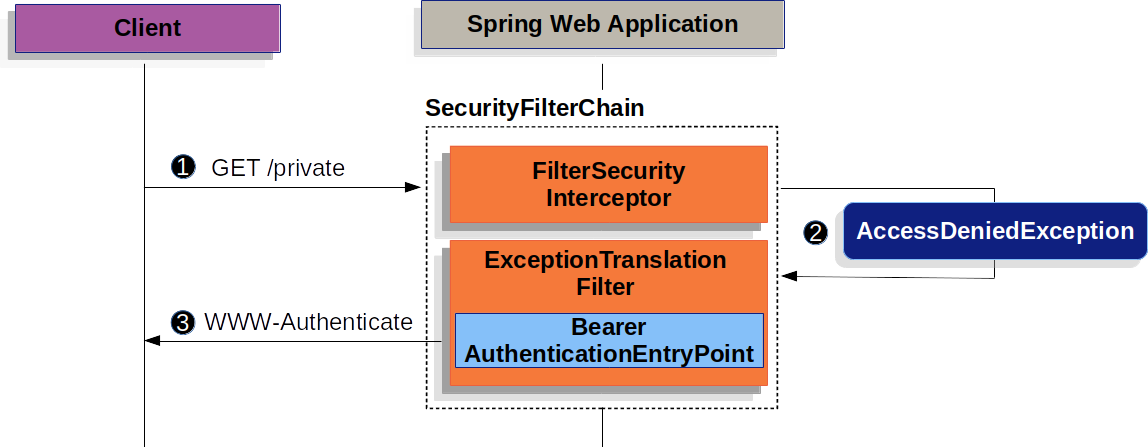
\includegraphics[width=1.0\textwidth]{gfx/bearerauthenticationentrypoint.png}
  \caption{Bearer Token Authentication \citep{springsecuritydoc:2021}}
  \label{fig:chapter03:bearerauthenticationentrypoint}
\end{figure}
\bigskip

In \autoref{fig:chapter03:bearerauthenticationentrypoint} ist die Funktionsweise der SecurityFilterChain abgebildet. In diesem Fall sendet ein Client eine Anfrage auf den durch OAuth2 geschützten Pfad /private der Spring Web Application. Falls die Anfrage nicht beantwortet werden darf, weil der Token des Clients invalide oder überhaupt kein Token vorhanden ist, wird eine AccessDeniedException geworfen und der Client wird aufgefordert sich zu authentifizieren. Ein valider Token, den der Client an den Server sendet, entspricht konzeptionell einer Authentifikation. 
Damit die Ressource Server die Tokens validieren können, musste der JSON Web Key Set Endpunkt des Authorization Server in der Spring-Boot-Applikation angegeben werden. Dadurch kann die Applikation sich die öffentlichen Schlüssel der RSA-Signatur von diesem Endpunkt holen und damit die RSA-Signatur validieren, indem aus dem durch Base64 kodierten Header und Payload des JSON Web Tokens die Signatur berechnet und auf Gleichheit überprüft wird. Da der Ressource Server auf derselben Host-Maschine wie Keycloak, der Authorization Server, läuft, ist der Endpunkt in diesem Fall also:

\begin{lstlisting}
  HTTP://localhost:9080/auth/realms/sample/protocol/openid-connect/certs
\end{lstlisting}
\smallskip

Zudem werden die folgenden Claims des JSON Web Tokens validiert:
\begin{itemize}
  \item exp
  \item nbf
  \item iss
\end{itemize}

Der exp-Claim (Expiration Time) ist derjenige Claim der angibt, bis wann der Token gültig ist.
Der nbf-Claim (Not Before) gibt den Zeitpunkt an, ab wann der Token akzeptiert werden darf.
Der iss-Claim (Issuer) gibt die \ac{URI} des Authorization Server an. Sie sollte dem Authorization Server entsprechen, von dem auch die öffentlichen Schlüssel für die RSA-Signatur geholt werden. 
In beiden Ressource Servern wird eine erfolgreiche Authentifizierung, also ein valider JSON Web Token, der von Keycloak erstellt wurde, erwartet. Die Autorisierung aber, also die Prüfung, ob der authentifizierte Nutzer die benötigten Rechte verfügt, um Zugriff auf die Schnittstelle zu erhalten, wird in den zwei Ressource Servern auf zwei unterschiedliche Weisen realisiert und in den nachfolgenden zwei Kapiteln beschrieben.

\subsection{Spring Security Ressource Server mit interner Zugriffskontrolle}

Um eine rollenbasierter Zugriffskontrolle in dem Ressource Server selbst zu realisieren, wurde JwtAuthenticationConverter verwendet, das Teil von Spring Security ist.

\begin{figure}[htbp]
  \centering
  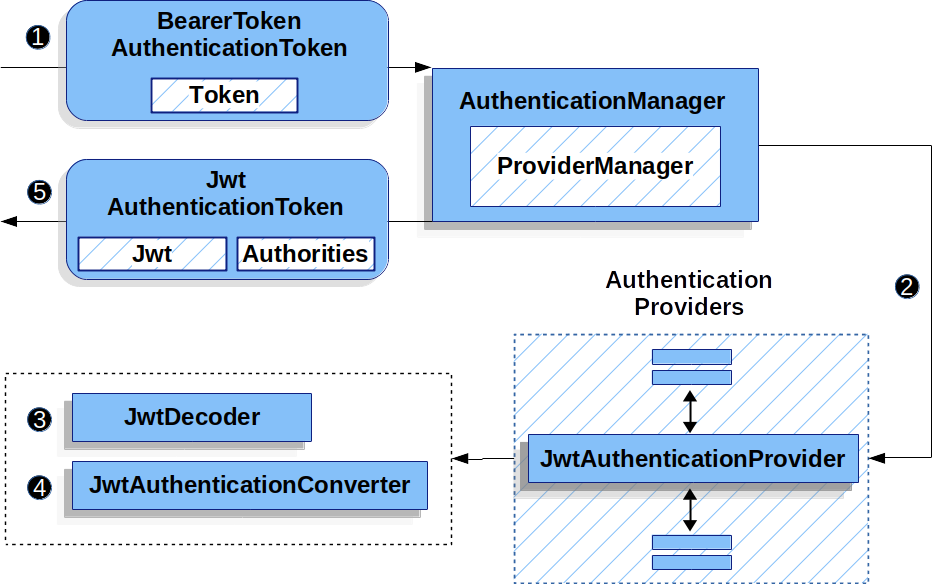
\includegraphics[width=1.0\textwidth]{gfx/jwtauthenticationprovider.png}
  \caption{JWT Authentication Provider \citep{springsecuritydoc:2021}}
  \label{fig:chapter03:jwtauthenticationprovider}
\end{figure}
\bigskip

In \autoref{fig:chapter03:jwtauthenticationprovider} ist der Ablauf dargestellt, um eine rollenbasierte Zugriffskontrolle in dem Server, also der Spring-Boot Applikation, mit dem JwtAuthenticationConverter zu realisieren. Im Wesentlichen wird hier der JSON Web Token durch den JWTAuthenticationProvider von einem JwtDecoder dekodiert, verifiziert und validiert und von dem JwtAuthenticationConverter werden Autoritäten in eine Collection gemappt. Als JwtDecoder wird die Nimbus Bibliothek verwendet \citep{springsecuritydoc:2021}.
Der JwtAuthenticationConverter wurde so konfiguriert, dass es Rollen aus dem JSON Web Token in sogenannte GrantedAuthorities mappt. Diese sind Objekte, die Privilegien von Nutzern widerspiegeln wie beispielsweise Rollen \citep{springsecuritydoc:2021}. 

\begin{lstlisting}[language=Java,frame=tb,caption={JwtAuthenticationConverter},label=lst:JwtAuthenticationConverter]
  @Bean
  public JwtAuthenticationConverter jwtAuthenticationConverter() {
      JwtGrantedAuthoritiesConverter grantedAuthoritiesConverter 
          = new JwtGrantedAuthoritiesConverter();
      grantedAuthoritiesConverter.setAuthoritiesClaimName("roles");
      grantedAuthoritiesConverter.setAuthorityPrefix("");        
  
      JwtAuthenticationConverter jwtAuthenticationConverter 
          = new JwtAuthenticationConverter();
      jwtAuthenticationConverter.
          setJwtGrantedAuthoritiesConverter(grantedAuthoritiesConverter);
      return jwtAuthenticationConverter;
  }    
\end{lstlisting}
\bigskip

In \autoref{lst:JwtAuthenticationConverter} ist die verwendete Konfiguration dargestellt. Es wird also in dem JSON Web Token, der von dem Client gesendet wurde, nach dem Claim roles in dem Payload des Tokens gesucht und die Werte, die darin enthalten sind in GrantedAuthorities konvertiert. In dem Claim roles steht unter anderem auch die Rolle des Nutzers, der sich bei Keycloak authentifiziert hat, und zwar ROLE\_USER. Siehe Abbildung 13 Keycloak Access Token.
Um die Schnittstelle aus \autoref{subsec:Schnittstelle} nur Nutzern zugänglich zu machen, die die Autorität ROLE\_USER besitzen, wurde HTTPSecurity verwendet, das Teil von Spring Security ist. 

\begin{lstlisting}[language=Java,frame=tb,caption={HTTPSecurity},label=lst:HTTPSecurity]
  @Override
  protected void configure(HTTPSecurity HTTP) throws Exception {
      HTTP
          .authorizeRequests(authorize -> authorize
              .mvcMatchers("/documents").hasAuthority("ROLE_USER")
              .anyRequest().permitAll()
          )   
          .oauth2ResourceServer(OAuth2ResourceServerConfigurer::jwt);
  } 
\end{lstlisting}
\bigskip

In \autoref{lst:HTTPSecurity} sieht man die verwendete Konfiguration. Hierbei wurde konfiguriert, dass auf den Pfad /documents nur zugegriffen werden darf, wenn dem anfragenden Client die GrantedAuthority ROLE\_USER zugewiesen wurde. 

\subsection{Spring Security Ressource Server mit externer Zugriffskontrolle}
Um die Zugriffskontrolle von dem zweiten Ressource Server zu entkoppeln, wurde der AccessDecisionManager verwendet, der Teil von Spring Security ist und es erlaubt Zugriffsentscheidungen externen Programmen zu überlassen. 
Als externes Programm um diese Zugriffsentscheidungen zu fällen, wurde Open Policy Agent in der Version 0.30.2 verwendet, das in einem Docker-Container ausgeführt wird und auf dem gleichen Host wie der Ressource Server läuft. 

\subsubsection{Rollenbasierte Zugriffskontrolle mit Open Policy Agent}
Zunächst wird die Systemarchitektur dargestellt, die das Zusammenspiel zwischen dem Authorization Server, Keycloak, dem Ressource Server, der Spring-Boot Applikation und dem Open Policy Agent erklärt. 

\begin{figure}[htbp]
  \centering
  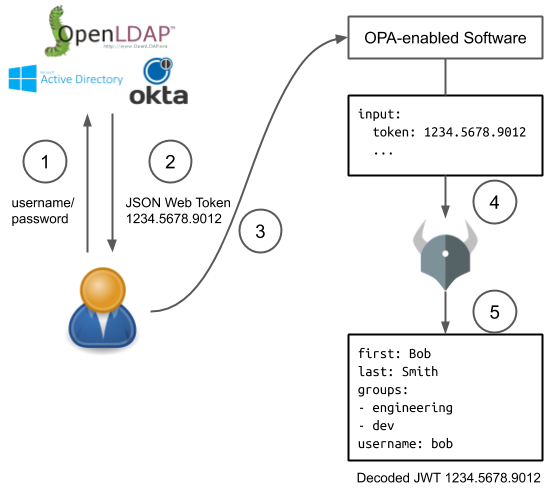
\includegraphics[width=0.75\textwidth]{gfx/data-jwt.png}
  \caption{Open Policy Agent und OAuth2 \citep{opaexternaldata:2021}}
  \label{fig:chapter03:data-jwt}
\end{figure}
\bigskip

In \autoref{fig:chapter03:data-jwt} ist die Systemarchitektur dargestellt. Zunächst authentifiziert sich der End-Nutzer bei dem Authorization Server. Hier ist als Beispiel Okta dargestellt, in diesem System wird allerdings Keycloak verwendet. Nachdem sich der End-Nutzer authentifiziert hat, erhält der Client einen JSON Web Token.
Mit diesem JSON Web Token sendet der Client eine Anfrage an die OPA-enabled Software. Dies ist der Ressource Server, also die Spring-Boot Applikation. 
Um eine Zugriffsentscheidung zu evaluieren, muss die OPA-enabled Software nun also die angefragte Schnittstelle inklusive Input-Daten an Open Policy Agent senden. Diese Input-Daten sind die JSON Web Token, in welchem unter anderem auch Nutzerattribute vorhanden sind, anhand dessen Open Police Agent mithilfe programmierter Zugriffsrichtlinien in Rego, eine Zugriffsentscheidung trifft und diese der OPA-enabled Software mitteilt, woraufhin der Client dann eine Antwort auf seine Anfrage erhält basierend auf der Zugriffsentscheidung von Open Policy Agent. 

\begin{lstlisting}[frame=tb,caption={Rollenbasierte Zugriffsrichtlinie in Rego},label=lst:RollenbasierteZugriffsrichtlinieinRego]
  package HTTP.authz

  default allow = false
  
  allow {
      input.method == "GET"
      input.path == ["documents"]
      token.payload.roles[_] == "ROLE_USER"
  }
  
  allow {
      input.method == "GET"
      input.path == ["h2-console"]
  }
  
  # Helper to get the token payload.
  token = {"payload": payload} {
      [header, payload, signature] := io.jwt.decode(input.auth.token.tokenValue)  
  }
\end{lstlisting}
\bigskip

In \autoref{lst:RollenbasierteZugriffsrichtlinieinRego} ist die verwendete programmierte rollenbasierte Zugriffskontrolle in Rego, der Programmiersprache von Open Policy Agent, um Zugriffsrichtlinien zu definieren, dargestellt. 
Es wird zunächst der JSON Web Token, den Open Policy Agent von dem Ressource Server erhält, dekodiert, da JSON Web Token in Base64 kodiert sind. Neben dem Token wird Open Policy Agent auch die angefragte HTTP-Schnittstelle mitgeteilt. 
In der ersten allow Methode, wird definiert, dass auf eine GET-Anfrage auf den Pfad documents, nur Zugriff erhalten werden darf, falls in dem Payload des JSON Web Token der Claim roles vorhanden ist und in diesem Claim der Wert ROLE\_USER vorhanden ist. Falls dem so ist, wird dem Ressource Server mitgeteilt, dass der Client autorisiert ist, eine Antwort auf seine Anfrage zu erhalten. 
Die zweite allow-Methode wird hier nicht weiter erläutert. Anfragen, die nicht der Schnittstelle documents oder h2-console entsprechen, werden grundsätzlich abgelehnt. 

\subsubsection{Spring Security AccessDecisionManager}
Um dem Ressource Server, Open Policy Agent die Zugriffsentscheidungen zu überlassen, wurde der AccessDecisionManager verwendet, der Teil von Spring Security ist. 

\begin{figure}[htbp]
  \centering
  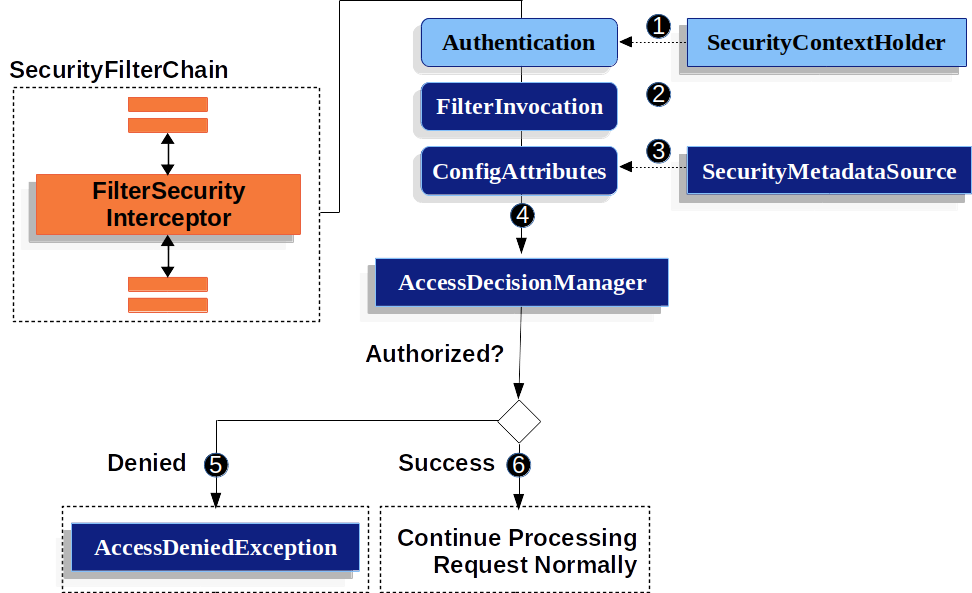
\includegraphics[width=1.0\textwidth]{gfx/filtersecurityinterceptor.png}
  \caption{AccessDecisionManager in Spring Security \citep{springsecuritydoc:2021}}
  \label{fig:chapter03:filtersecurityinterceptor}
\end{figure}
\bigskip

In \autoref{fig:chapter03:filtersecurityinterceptor} ist die Funktionsweise dargestellt. Zunächst durchläuft die ankommende Anfrage des Clients die SecurityFilterChain. Im Fall einer erfolgreichen Authentifikation, was im Falle von OAuth2 einer erfolgreichen Validierung des JSON Web Tokens entspricht, trifft der AccessDecisionManager eine Zugriffsentscheidung. 
In dem AccessDecisionManager-Objekt wurde die Funktion vote() implementiert, die eine HTTP-Verbindung mit dem Open Policy Agent aufbaut, der auf der gleichen Host-Maschine wie die Spring-Boot Applikation läuft, um eine möglichst geringe Latenz zwischen beiden Programmen zu haben. Dies würde man in den allermeisten Anwendungsszenarien auch im Produktiveinsatz machen, da Open Policy Agent äußerst leichtgewichtig ist in der Belegung des Arbeitsspeichers. Die vote()-Funktion, sendet Open Policy Agent alle nötigen Informationen, damit dieser anhand dieser Informationen mit der programmierten Zugriffsrichtlinie eine Zugriffsentscheidung treffen kann, also:

\begin{itemize}
  \item Der Pfad auf den der Client zugreifen möchte
  \item Die HTTP-Methode, mit der der Client auf diesen Pfad zugreifen möchte (GET, PUT, POST etc.)
  \item Die Input-Daten, also der in Base64-kodierte JSON Web Token, welcher in dem SecurityContextHolder-Objekt gespeichert wird
\end{itemize}

Daraufhin wird dem Ressource Server dann von dem AccessDecisionManager, also Open Policy Agent, eine Zugriffsentscheidung per HTTP mitgeteilt. Anhand dieser Entscheidung erlaubt oder verweigert der Ressource Server dem Client den Zugriff auf die Schnittstelle. 
Es wurde nun also beide Ressource Server mit ihrer jeweiligen Zugriffskontrolle beschrieben. 

\section{Performancetests mit Apache JMeter}
Um Performancetests auf beiden Ressource Server durchzuführen und die Ergebnisse vergleichend auszuwerten, um den Einfluss von externer Zugriffskontrolle mit Open Policy Agent auf OAuth2 Ressource Server zu untersuchen, wurde Apache JMeter in der Version 5.4.1 verwendet. Mit Apache JMeter ist es möglich durch die Verwendung von Threads, Nutzer zu simulieren, die HTTP-Anfragen an einen Server senden. In diesen HTTP-Anfragen wird jeweils ein valider JSON Web Token an die Ressource Server gesendet und diese evaluieren dann jeweils eine Zugriffsentscheidung. Es wird gemessen, wie lange die Ressource Server jeweils für eine Evaluierung einer Zugriffsentscheidung und das darauffolgende Senden der Antwort benötigen.\smallskip

Wenn ein Single Sign-On mittels OpenID Connect implementiert wird, senden eingeloggte Nutzer bei jeder Anfrage den JSON Web Token, den sie nach der Authentifikation von dem Authorization Server erhalten haben an den Ressource Server, um Zugriff auf dessen Schnittstellen zu erhalten. Bei diesen Performancetests werden also eingeloggte Nutzer simuliert, die auf Schnittstellen eines Servers zugreifen möchten. Jeder Thread entspricht einem eingeloggten Nutzer.\smallskip

Es wurden drei Testpläne erstellt, die verschiedene Aspekte der Server testen, wobei alle drei unter dem Überpunkt der Performance gehören. Die drei Testpläne werden als Lasttest, Skarlierbarkeitstest und Stresstest bezeichnet. 

\begin{description}
  \item[Lasttest:] Bei dem Lasttest wird der Server mit üblicher Last getestet und die Latenz gemessen. 
  \item[Skalierbarkeitstest:] Bei dem Skalierbarkeitstest wird ansteigende Last auf dem Server generiert, wobei hierbei untersucht werden soll, inwiefern sich Antwortzeiten des Servers bei hinzukommender Last ändern. 
  \item[Stresstest:] Bei dem Stresstest wird eine unüblich hohe Last auf den Server generiert, um die Grenzen des Servers feststellen zu können. 
\end{description}

Bei jedem Test wird auch die \ac{CPU}-Auslastung und Arbeitsspeicherbelegung betrachtet. Alle Tests wurden verteilt gestartet, das bedeutet, dass Client (Apache JMeter) und Server auf jeweils einem Rechner laufen. Dies dient dem Zweck, dass die Testergebnisse nicht verfälscht werden, da bei einer hohen Anzahl von Threads sowohl das Senden von HTTP-Anfragen CPU-Last erzeugt als auch das Abarbeiten der Anfragen durch den Server und beide Prozesse sich gegenseitig nicht ausbremsen sollten. Die verwendete Systemhardware von Client und Server, ist in \autoref{subsec:SystemhardwareundTestumfeld} zu sehen.

\subsection{Lasttest}
In dem Lasttest wurde eine übliche Last auf den Server generiert und mittels sogenannten Listener die Ergebnisse gemessen und protokolliert. 

\begin{figure}[htbp]
  \centering
  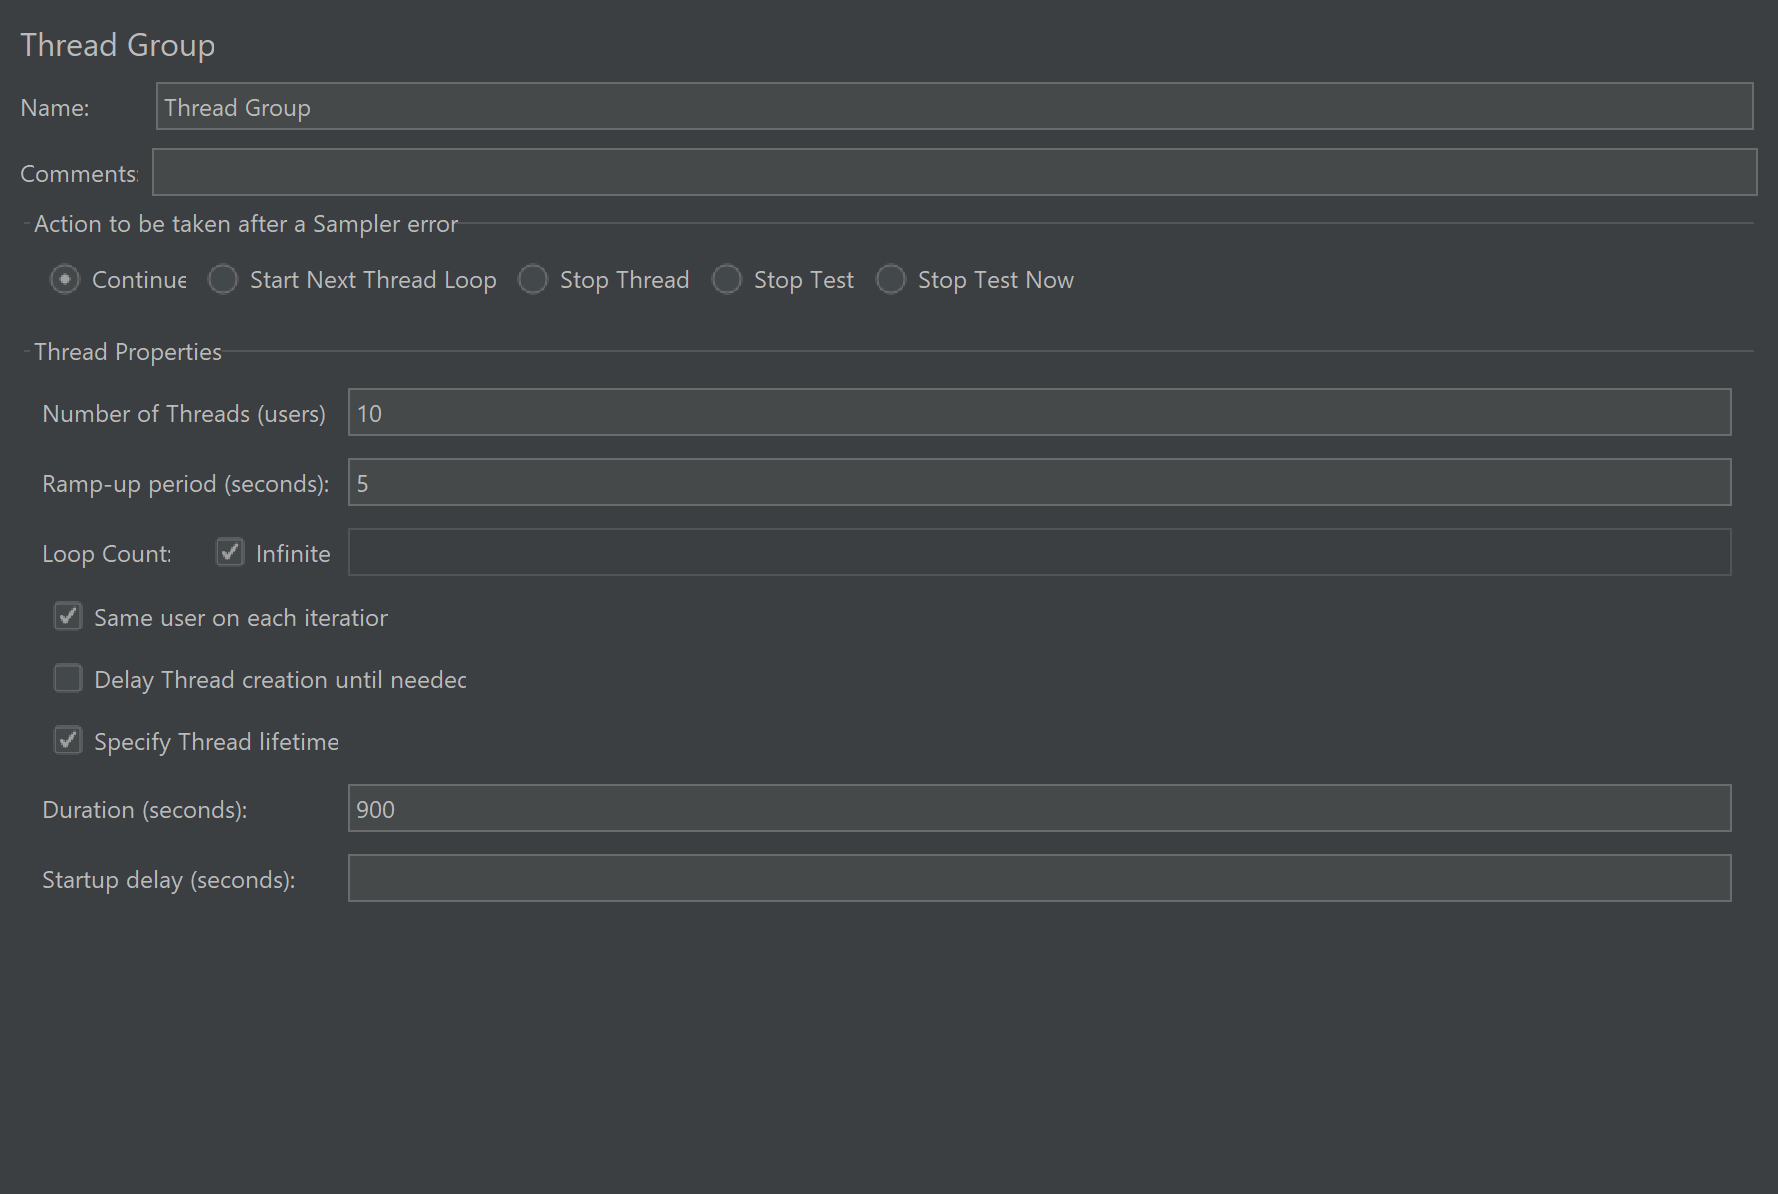
\includegraphics[width=1.0\textwidth]{gfx/Thread Group-Last.png}
  \caption{Thread Group-Last}
  \label{fig:chapter03:ThreadGroup-Last}
\end{figure}
\bigskip

In \autoref{fig:chapter03:ThreadGroup-Last} ist die verwendete Konfiguration dargestellt. Es werden zehn Threads gestartet, die jeweils gleichzeitig HTTP-Anfragen an den Server senden. Als Ramp-up period wurde fünf Sekunden gesetzt. Das bedeutet, es dauert fünf Sekunden, bis alle zehn Threads gestartet sind. Als Duration ist 900 Sekunden eingestellt worden, das bedeutet das der Test 15 Minuten dauert. 

\begin{figure}[htbp]
  \centering
  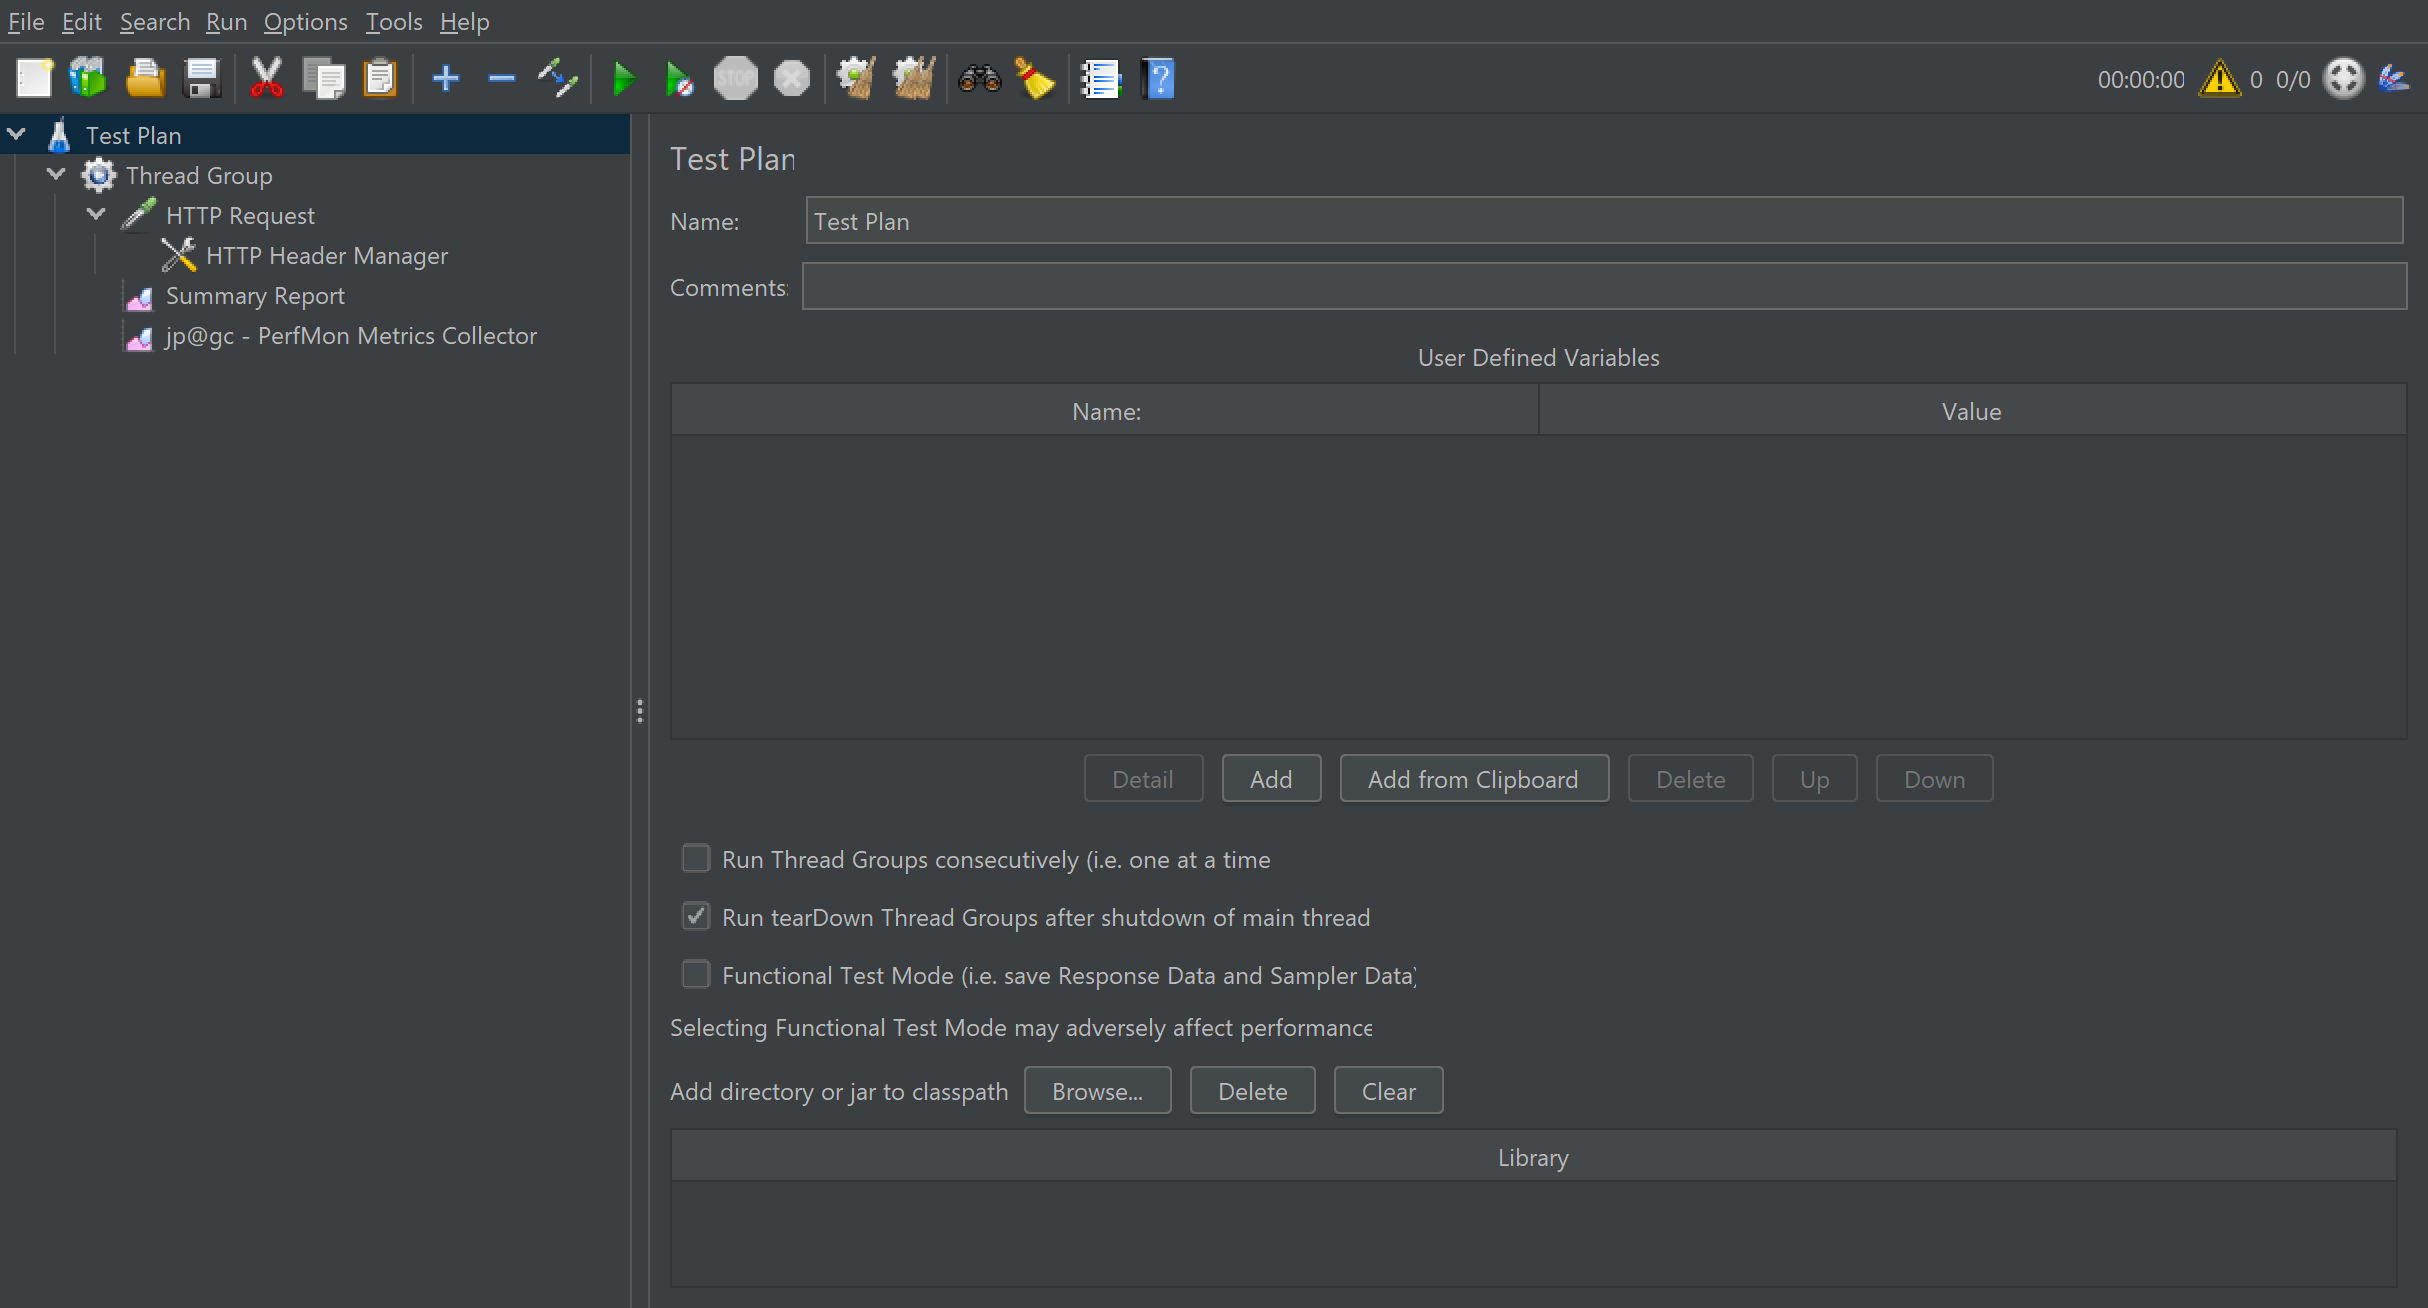
\includegraphics[width=1.0\textwidth]{gfx/Test Plan-Last.png}
  \caption{Test Plan-Last}
  \label{fig:chapter03:TestPlan-Last}
\end{figure}
\bigskip

In \autoref{fig:chapter03:TestPlan-Last} ist eine Gesamtübersicht des Testplans dargestellt. In Thread Group wurde die Konfiguration vorgenommen, die in Abbildung 22 dargestellt ist. Hier wurden zwei Listener konfiguriert, nämlich Summary Report und jp@gc – Performance Metrics Collector. Summary Report ist für das Protokollieren der Messdaten zuständig. Hier werden unter anderem die Latenz, Response Time und Connect Time protokolliert. Der Performance Metrics Collector ist für das Messen von CPU-Auslastung und RAM-Belegung zuständig.
In dem HTTP Header Manager wird der HTTP-Header der HTTP-Anfrage, die jeweils an den Server gesendet werden soll, konfiguriert. 

\begin{figure}[htbp]
  \centering
  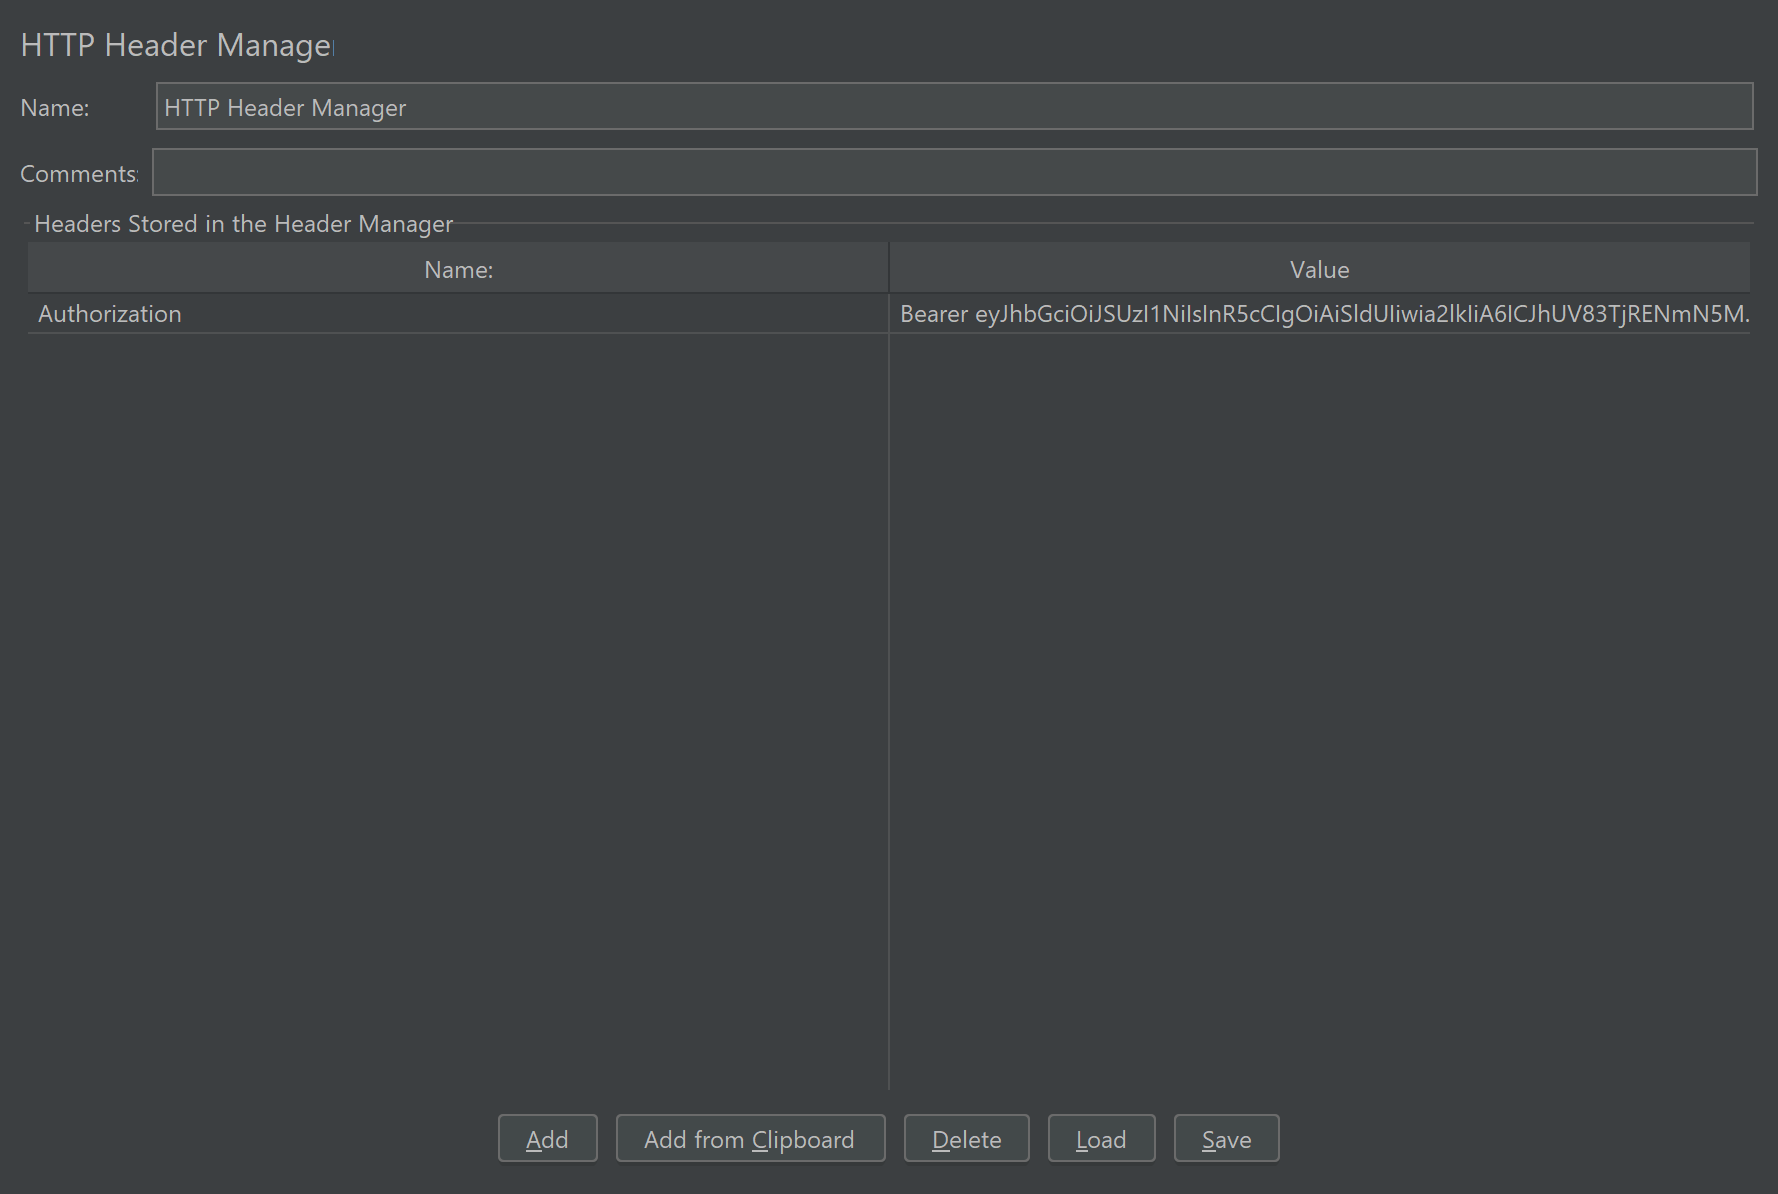
\includegraphics[width=1.0\textwidth]{gfx/HTTP Header Manager.png}
  \caption{HTTP Header Manager}
  \label{fig:chapter03:HTTPHeaderManager}
\end{figure}
\bigskip

In \autoref{fig:chapter03:HTTPHeaderManager} ist der verwendete HTTP Header Manager zu sehen. Hier wurde lediglich der JSON Web Token in dem Schlüssel Authorization des HTTP-Headers hinterlegt. Der Erhalt des Tokens wurde in Kapitel 3.2 beschrieben. Als Prefix wird Bearer angegeben, um dem empfangenden System zu signalisieren, dass in dem Authorization-Feld des HTTP-Headers ein Bearer Token steht, also ein durch OAuth2 Code Grant erlangter Token [8].

\begin{figure}[htbp]
  \centering
  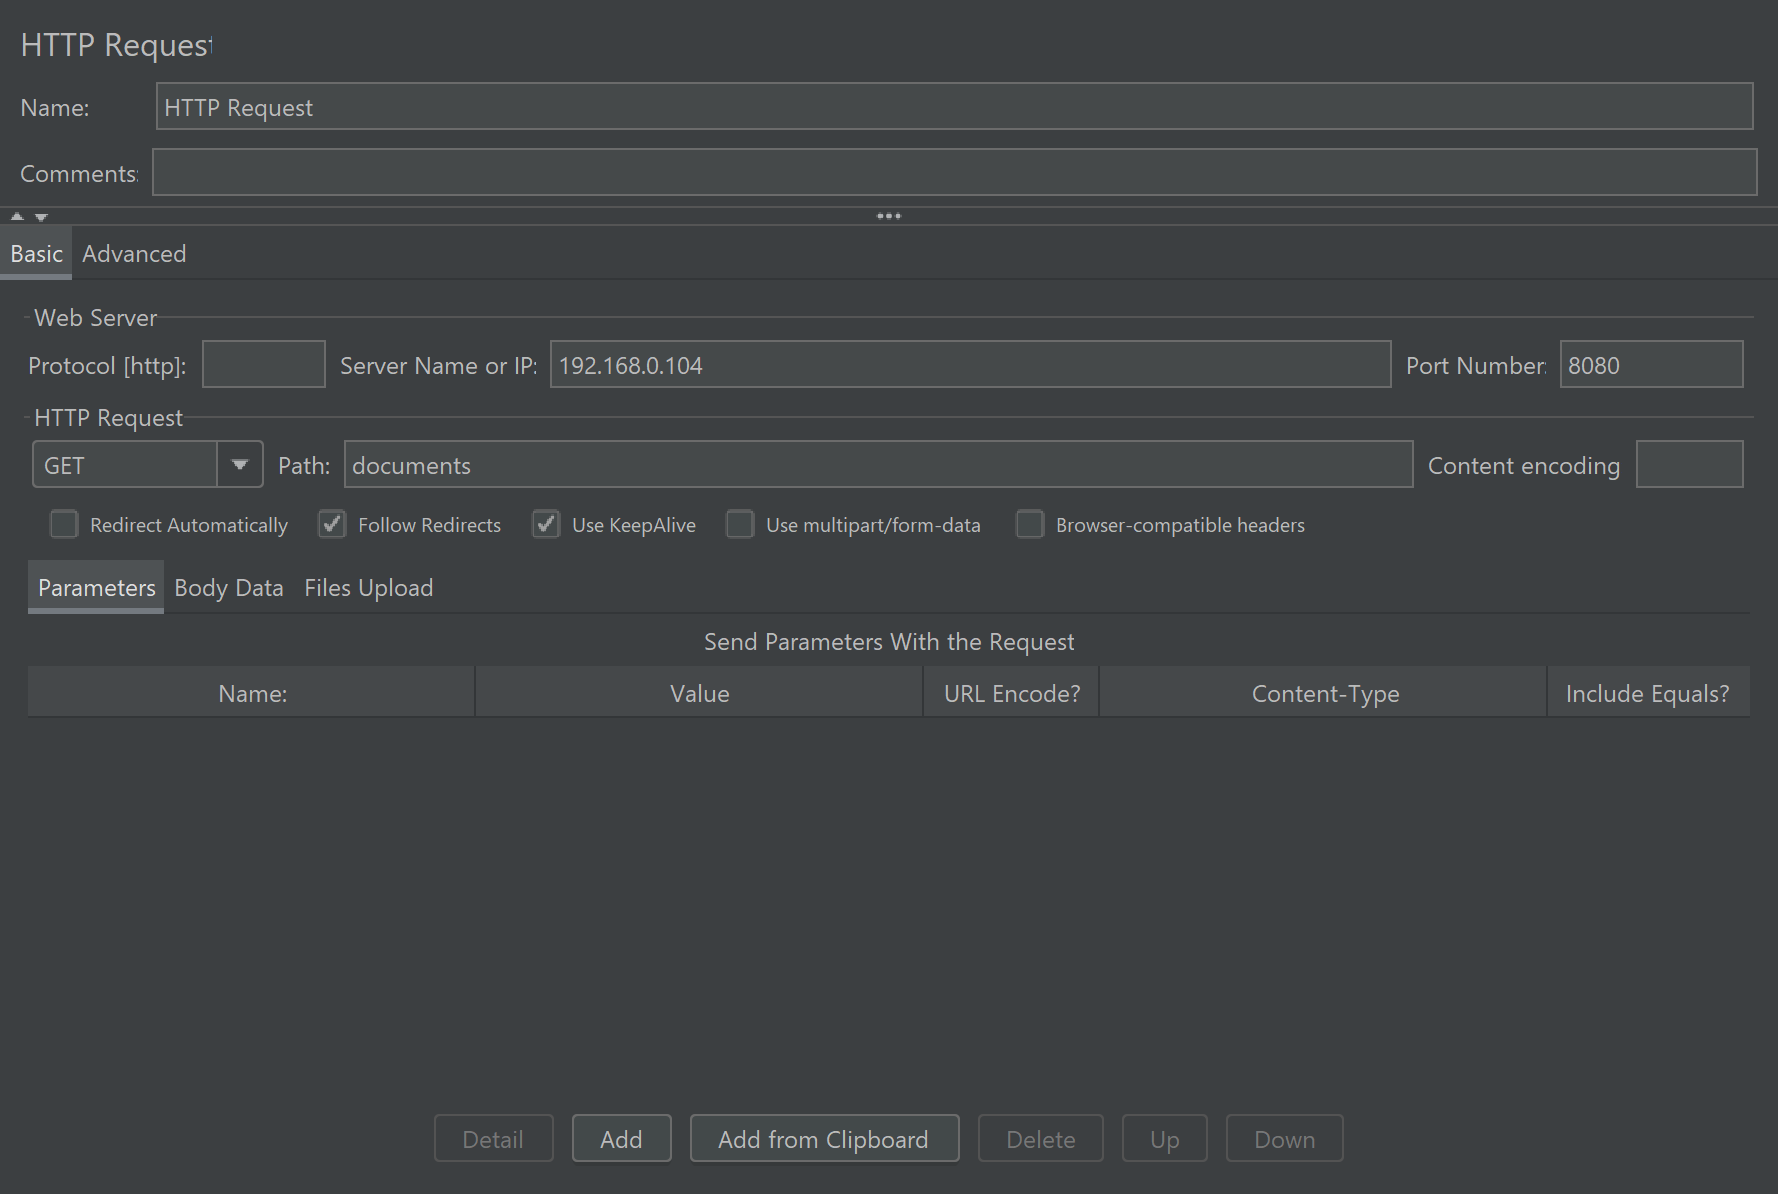
\includegraphics[width=1.0\textwidth]{gfx/HTTP Request.png}
  \caption{HTTP Request}
  \label{fig:chapter03:HTTPRequest}
\end{figure}
\bigskip

In \autoref{fig:chapter03:HTTPRequest} ist die HTTP-Anfrage zu sehen, die jeweils an den Server gesendet wird. Hier wurde die Anfragemethode auf GET eingestellt und der Pfad auf documents gesetzt, denn die Schnittstelle des Ressource Server ist wie in Kapitel 3.3.1 erläutert eine HTTP-GET-Schnittstelle. In dem Feld Server Name or IP wurde die IP-Adresse des Servers angegeben. Bei den Tests wird Client, also Apache JMeter, und Server auf zwei Rechnern gestartet, damit die Testergebnisse nicht verfälscht werden. 

\subsection{Skalierbarkeitstest}
Bei dem Skalierbarkeitstest geht es darum, eine ansteigende Last zu generieren, um herauszufinden inwiefern sich die Latenzen verändern. Je mehr Last erzeugt wird, desto höher werden tendenziell die Latenzen. 

\begin{figure}[htbp]
  \centering
  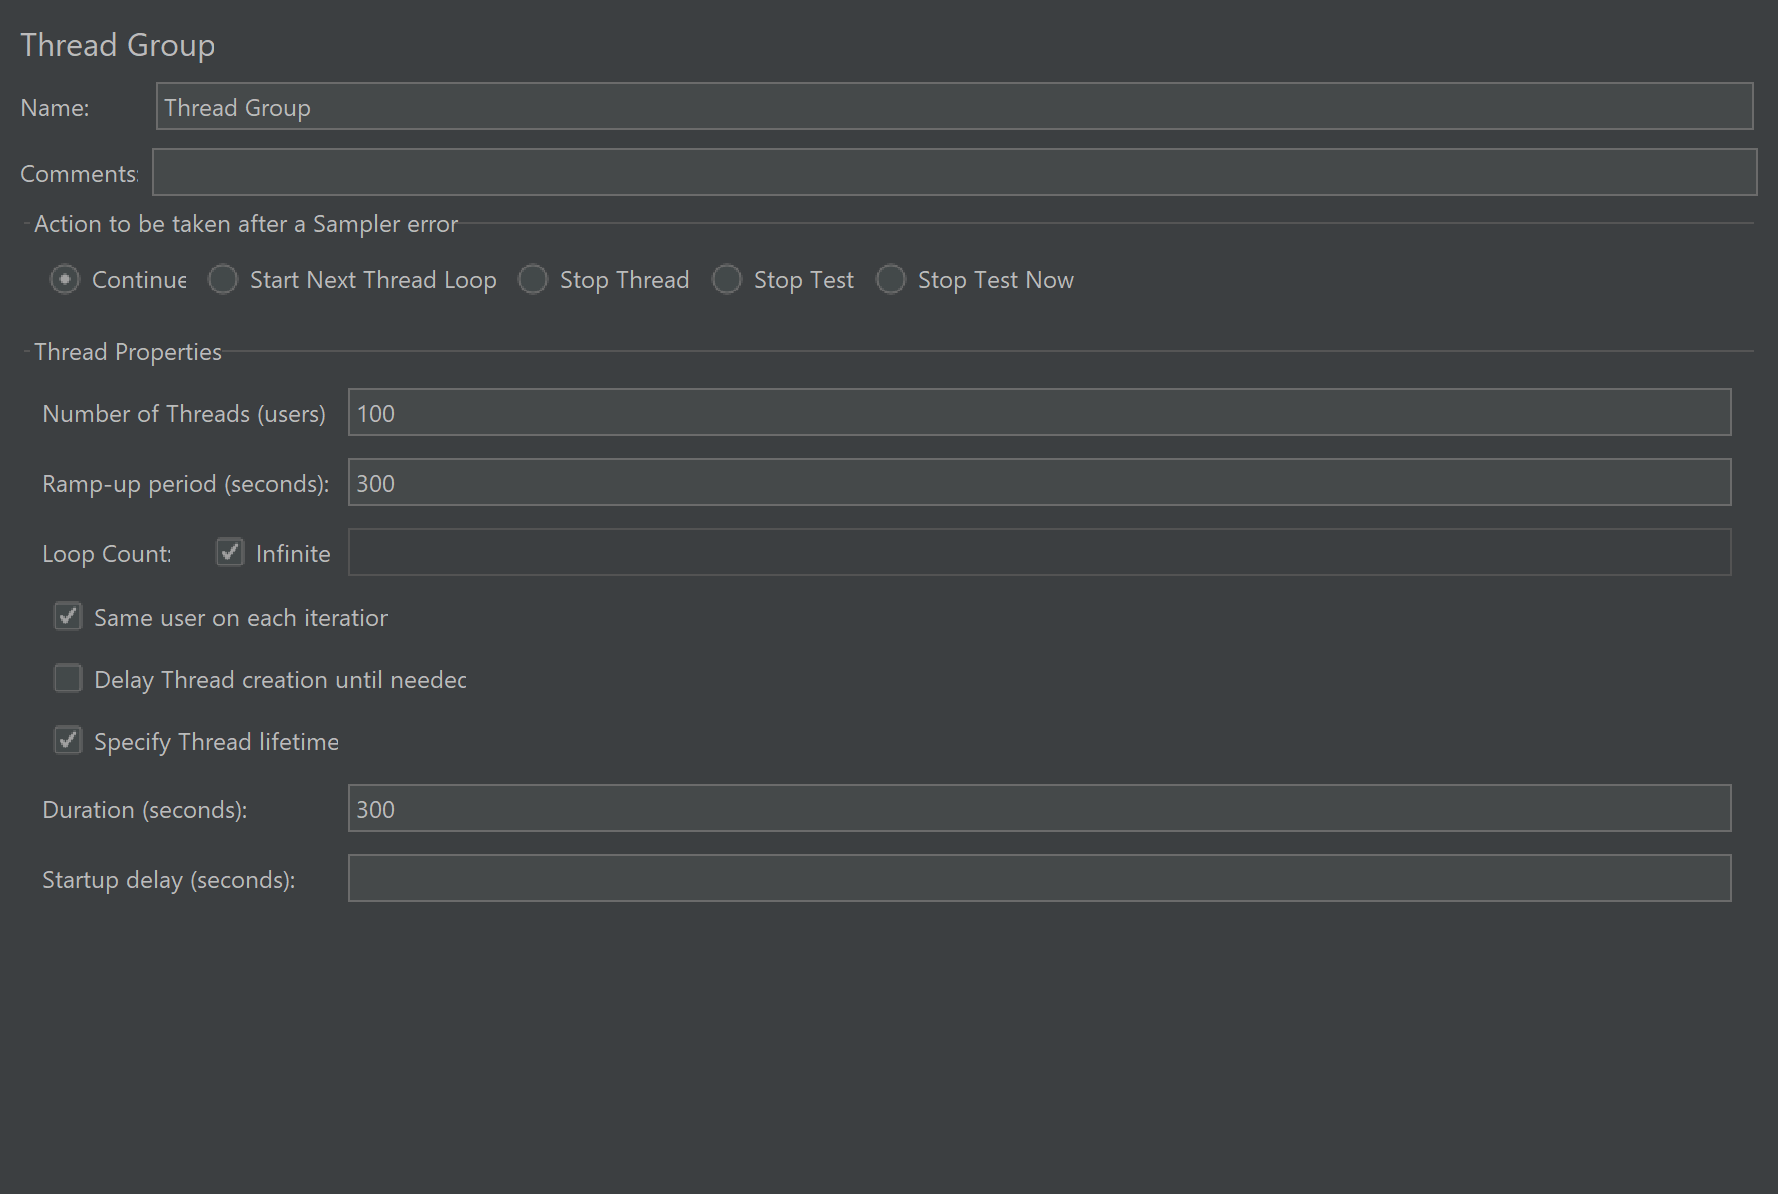
\includegraphics[width=1.0\textwidth]{gfx/Thread Group-Skalierung.png}
  \caption{Thread Group-Skalierung}
  \label{fig:chapter03:ThreadGroup-Skalierung}
\end{figure}
\bigskip

In \autoref{fig:chapter03:ThreadGroup-Skalierung} ist die verwendete Konfiguration zu sehen. Es werden 100 Threads gestartet, wobei hier die Ramp-up period 300 beträgt, dass bedeutet das erst nach 300 Sekunden alle 100 Threads gestartet wurden. Es werden also pro Sekunde 300/100 = 3 Threads gestartet. Die Gesamtdauer des Tests beträgt 300 Sekunden, also 15 Minuten. 
Was dadurch ermöglicht wird, ist das bis zum Ende des Tests eine ansteigende Last auf den Server entsteht. Dadurch lässt sich dann betrachten, inwiefern sich die Latenzen beziehungsweise Response Times der Anfragen bei ansteigender Last verhalten. 

\subsection{Stresstest}
Bei dem Stresstest geht es darum, dass eine möglichst hohe Last auf den Server erzeugt wird, um die Grenzen des Systems auszuloten. Dies ist wichtig, da man in der Regel wissen will, wie viele Nutzer ein System gleichzeitig bedienen kann, bis das System entweder unerreichbar wird oder die Latenzen der Antworten unakzeptabel hoch sind, damit man dem zum geeigneten Zeitpunkt durch horizontale Skalierung entgegenwirken kann. Zudem können durch diesen Test, Schwachstellen der jeweiligen Implementierungen wie beispielsweise Memory Leaks, erkannt werden. 

\begin{figure}[htbp]
  \centering
  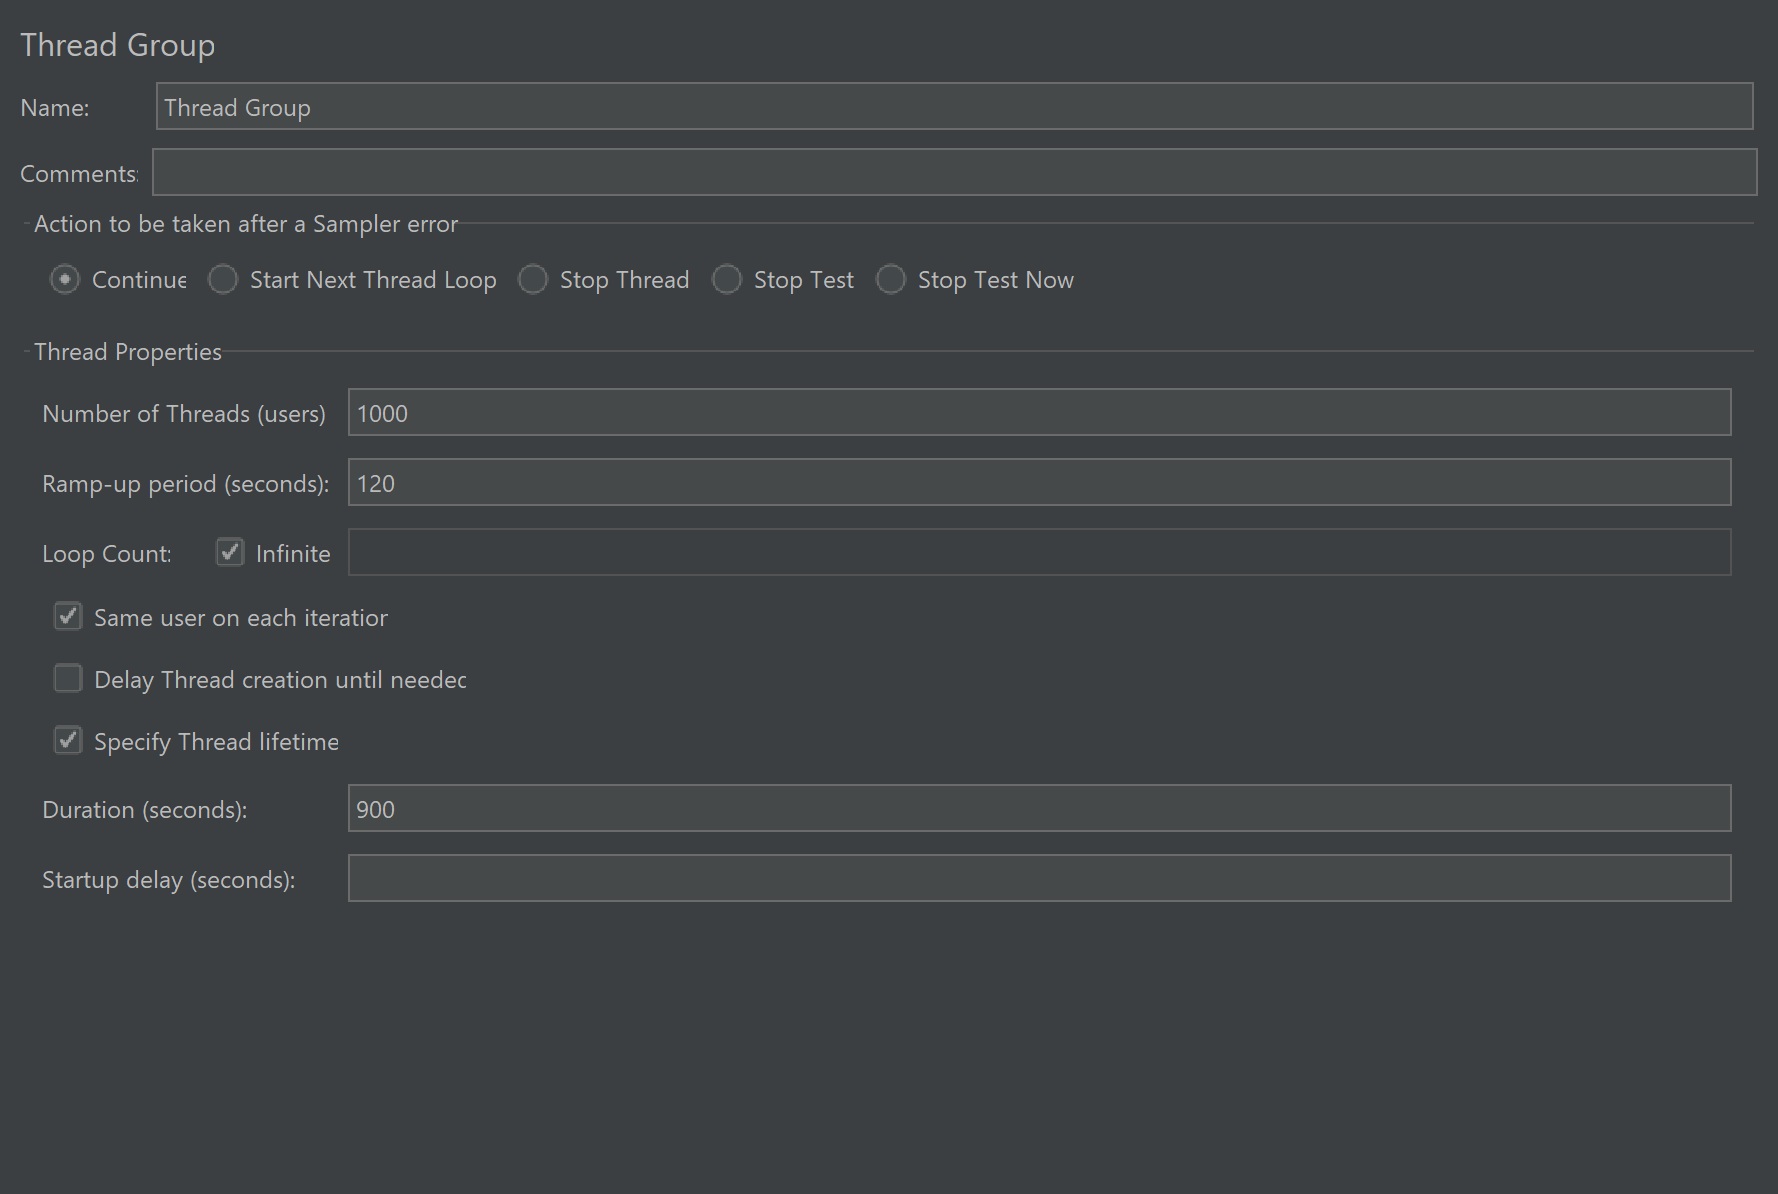
\includegraphics[width=1.0\textwidth]{gfx/Thread Group-Stress.png}
  \caption{Thread Group-Stress}
  \label{fig:chapter03:ThreadGroup-Stress}
\end{figure}
\bigskip

In \autoref{fig:chapter03:ThreadGroup-Stress} ist die verwendete Konfiguration zu sehen. Es werden insgesamt 1000 Threads gestartet wobei alle 1000 Threads erst nach 120 Sekunden gestartet sind. Der Test dauert insgesamt 900 Sekunden, das heißt 15 Minuten. Während dieser Zeit sendet jeder Thread kontinuierlich Anfragen an den Server. Dieser Test ist also deutlich ressourcenintensiver als der Last-und-Skalierbarkeitstest. Verlässlich können pro Maschine in Apache JMeter, ca. 1000-2000 Threads gestartet werden, was allerdings abhängig ist von der jeweiligen Hardware des Systems, auf dem Apache JMeter ausgeführt wird \citep{jmetermaxthreads:2017}. Dieser Test wird ohne die GUI von Apache JMeter ausgeführt, da diese speziell bei ressourcenintensiven Stresstests die Testergebnisse verfälschen kann. Die verwendete Systemhardware von Client und Server werden im Kapitel Systemhardware beschrieben. 

\subsection{Messung und Protokollierung von Messdaten}
Um die Messdaten der Tests aus den vorrangegangenen Kapiteln zu protokollieren und in geeigneter Weise zu visualisieren, wurden Apache JMeter Listener verwendet, die Messdaten in Comma-separated values (CSV)-Dateien schreiben. Um diese Daten visuell darzustellen, wurde der HTML Report von Apache JMeter verwendet. Als Listener wurde jeweils Summary Report verwendet. Dieser misst und protokolliert unter anderem die folgenden Daten: 
\begin{itemize}
  \item Response Time
  \item HTTP-Status Code der Antwort des Servers
  \item Latenz
  \item Connect Time
  \item Gesendete Bytes
  \item Erhaltene Bytes
\end{itemize}
\smallskip

Für die Bestimmung des Application Performance Index wurden folgende Werte gewählt:

\begin{table}[h]
  \myfloatalign
  \begin{tabularx}{\textwidth}{|l|l|X|} \toprule
      \tableheadline{Level} & \tableheadline{Multiplier} & \tableheadline{Time T} \\ \midrule
      Zufrieden & <= T & <= 500 Millisekunden  \\
      \midrule
      Toleriert & >T, <= 3T & [0,5 Sekunden, 1,5 Sekunden]  \\
      \midrule
      Frustriert & > 3T & > 1,5 Sekunden  \\
      \bottomrule
  \end{tabularx}
  \caption[Application Performance Index]{Application Performance Index.}
  \label{tab:ApplicationPerformanceIndex2}
\end{table}

Das bedeutet, dass Nutzer bis zu einer Response Time von 500 Millisekunden zufrieden sind. Response Times bis 1500 Millisekunden tolerieren Nutzer und bei Response Times ab 1500 Millisekunden sind Nutzer frustriert. Der Multiplier ist hier also 3T. Aus diesen Werten wird dann also der Performance Index berechnet.

\section{Systemhardware und Testumfeld}
\label{subsec:SystemhardwareundTestumfeld}
Es wird die verwendete Systemhardware für Client und Server, die in allen drei Tests verwendet wurde, aufgelistet. Dies ist erwähnenswert, da die Messwerte von der Leistungsfähigkeit der Hardware abhängen. Da allerdings ein Vergleich zwischen zwei Systemen gezogen wird, können auch allgemeingültige Erkenntnisse aus den Ergebnissen der Tests gezogen werden. Ein weiterer wichtige Punkt ist der, dass beide Rechner, also Client und Server, sich in demselben Netzwerk befinden und über denselben Router über Ethernet mit dem Internet verbunden sind. 
Open Policy Agent wird in einem Docker-Container ausgeführt und für die Simulierung der virtuellen Maschine des Docker-Containers wird \ac{WSL 2} verwendet. Für die Ressourcenbereitstellung des Docker-Containers, wurden die Standardeinstellungen verwendet. Diese sind in der Dokumentation von Microsoft vorzufinden \citep{wsl:2021}. Das bedeutet, der Docker-Container kann alle Prozessorkerne verwenden und ist bei der Arbeitsspeicherbelegung auf 8 Gigabyte begrenzt. 

\begin{table}[h]
  \myfloatalign
  \begin{tabularx}{\textwidth}{|l|X|} \toprule
      \tableheadline{Komponente} & \tableheadline{Spezifikation} \\ \midrule
      CPU & Intel(R) Core(TM) i5-8265U CPU @ 1.60GHz \\
      \midrule
      Arbeitsspeicher & 16 Gigabyte \\
      \midrule
      Betriebssystem & Microsoft Windows 10 Pro, 64 Bit Version	10.0.19042 Build 19042 \\
      \bottomrule
  \end{tabularx}
  \caption[System des Clients]{System des Clients.}
  \label{tab:SystemdesClients}
\end{table}

In \autoref{tab:SystemdesClients} ist das System des Clients dargestellt. Auf diesem System wird Apache JMeter ausgeführt, es sendet also jeweils die HTTP-Anfragen an den Server. 

\begin{table}[h]
  \myfloatalign
  \begin{tabularx}{\textwidth}{|l|X|} \toprule
      \tableheadline{Komponente} & \tableheadline{Spezifikation} \\ \midrule
      CPU & Intel(R) Core(TM) i7-7700HQ CPU @ 2.80GHz \\
      \midrule
      Arbeitsspeicher & 16 Gigabyte \\
      \midrule
      Betriebssystem & Microsoft Windows 10 Education, 64 Bit Version	10.0.19042 Build 19042 \\
      \bottomrule
  \end{tabularx}
  \caption[System des Servers]{System des Servers.}
  \label{tab:SystemdesServers}
\end{table}

In \autoref{tab:SystemdesServers} ist das System des Servers dargestellt. Hier laufen also die jeweiligen Ressource Server, die die Anfragen von Apache JMeter beantworten.
%*************************************************************************
% Recommendations
%*************************************************************************
%\part{Empfehlungen zur Erstellung wissenschaftlicher Abschlussarbeiten}
%\label{pt:recommendations}
%*************************************************************************
% Backmatter
%*************************************************************************
\appendix
%\renewcommand{\thechapter}{\alph{chapter}}
\cleardoublepage
\part{Appendix}
%************************************************
\chapter{Introduction to the ClassicThesis style}\label{ch:classicthesis}
%************************************************
The ClassicThesis bundle for \LaTeX\ has two goals:
\begin{enumerate}
    \item Provide students with an easy-to-use template for their
    Master's
    or PhD thesis. (Though it might also be used by other types of
    authors
    for reports, books, etc.)
    \item Provide a classic, high-quality typographic style that is
    inspired by \citeauthor{bringhurst:2002}'s ``\emph{The Elements of
    Typographic Style}'' \citep{bringhurst:2002}.
    \marginpar{\myTitle \myVersion}
\end{enumerate}
The bundle is configured to run with a \emph{full}
MiK\TeX\ or \TeX Live\footnote{See the file \texttt{LISTOFFILES} for
needed packages. Furthermore, \texttt{classicthesis}
works with most other distributions and, thus, with most systems
\LaTeX\ is available for.}
installation right away and, therefore, it uses only freely available
fonts. (Minion fans can easily adjust the style to their needs.)

People interested only in the nice style and not the whole bundle can
now use the style stand-alone via the file \texttt{classicthesis.sty}.
This works now also with ``plain'' \LaTeX.

As of version 3.0, \texttt{classicthesis} can also be easily used with
\mLyX\footnote{\url{http://www.lyx.org}} thanks to Nicholas Mariette
and Ivo Pletikosić. The \mLyX\ version of this manual will contain
more information on the details.

This should enable anyone with a basic knowledge of \LaTeXe\ or \mLyX\ to
produce beautiful documents without too much effort. In the end, this
is my overall goal: more beautiful documents, especially theses, as I
am tired of seeing so many ugly ones.

The whole template and the used style is released under the
\acsfont{GNU} General Public License.

If you like the style then I would appreciate a postcard:
\begin{center}
    André Miede \\
    Detmolder Straße 32 \\
    31737 Rinteln \\
    Germany
\end{center}
The postcards I received so far are available at:
\begin{center}
    \url{http://postcards.miede.de}
\end{center}
\marginpar{A well-balanced line width improves the legibility of
the text. That's what typography is all about, right?}
So far, many theses, some books, and several other publications have
been typeset successfully with it. If you are interested in some
typographic details behind it, enjoy Robert Bringhurst's wonderful book.
% \citep{bringhurst:2002}.

\paragraph{Important Note:} Some things of this style might look
unusual at first glance, many people feel so in the beginning.
However, all things are intentionally designed to be as they are,
especially these:
\begin{itemize}
    \item No bold fonts are used. Italics or spaced small caps do the
    job quite well.
    \item The size of the text body is intentionally shaped like it
    is. It supports both legibility and allows a reasonable amount of
    information to be on a page. And, no: the lines are not too short.
    \item The tables intentionally do not use vertical or double
    rules. See the documentation for the \texttt{booktabs} package for
    a nice discussion of this topic.\footnote{To be found online at
    \url{http://mirror.ctan.org/macros/latex/contrib/booktabs/}.}
    \item And last but not least, to provide the reader with a way
    easier access to page numbers in the table of contents, the page
    numbers are right behind the titles. Yes, they are \emph{not}
    neatly aligned at the right side and they are \emph{not} connected
    with dots that help the eye to bridge a distance that is not
    necessary. If you are still not convinced: is your reader
    interested in the page number or does she want to sum the numbers
    up?
\end{itemize}
Therefore, please do not break the beauty of the style by changing
these things unless you really know what you are doing! Please.

\paragraph{Yet Another Important Note:} Since \texttt{classicthesis}'
first release in 2006, many things have changed in the \LaTeX\ world.
Trying to keep up-to-date, \texttt{classicthesis} grew and evolved
into many directions, trying to stay (some kind of) stable and be
compatible with its port to \mLyX. However, there are still many
remains from older times in the code, many dirty workarounds here and
there, and several other things I am absolutely not proud of (for
example my unwise combination of \acsfont{KOMA} and
\texttt{titlesec} etc.).
\graffito{An outlook into the future of \texttt{classicthesis}.}

Currently, I am looking into how to completely re-design and
re-implement \texttt{classicthesis} making it easier to maintain and
to use. As a general idea, \texttt{classicthesis.sty} should be
developed and distributed separately from the template bundle itself.
Excellent spin-offs such as \texttt{arsclassica} could also be
integrated (with permission by their authors) as format configurations.
Also, current trends of \texttt{microtype}, \texttt{fontspec}, etc.
should be included as well. As I am not really into deep
\LaTeX\ programming,
I will reach out to the \LaTeX\ community for their expertise and help.


\section{Organization}
A very important factor for successful thesis writing is the
organization of the material. This template suggests a structure as
the following:
\begin{itemize}
    \marginpar{You can use these margins for summaries of the text
    body\dots}
    \item\texttt{Chapters/} is where all the ``real'' content goes in
    separate files such as \texttt{Chapter01.tex} etc.
    % \item\texttt{Examples/} is where you store all listings and other
    % examples you want to use for your text.
    \item\texttt{FrontBackMatter/} is where all the stuff goes that
    surrounds the ``real'' content, such as the acknowledgments,
    dedication, etc.
    \item\texttt{gfx/} is where you put all the graphics you use in
    the thesis. Maybe they should be organized into subfolders
    depending on the chapter they are used in, if you have a lot of
    graphics.
    \item\texttt{Bibliography.bib}: the Bib\TeX\ database to organize
    all the references you might want to cite.
    \item\texttt{classicthesis.sty}: the style definition to get this
    awesome look and feel. Does not only work with this thesis template
    but also on its own (see folder \texttt{Examples}). Bonus: works
    with both \LaTeX\ and \textsc{pdf}\LaTeX\dots and \mLyX.
    % \item\texttt{ClassicThesis.tcp} a \TeX nicCenter project file.
    Great tool and it's free!
    \item\texttt{ClassicThesis.tex}: the main file of your thesis
    where all gets bundled together.
    \item\texttt{classicthesis-config.tex}: a central place to load all
    nifty packages that are used. % In there, you can also activate
    % backrefs in order to have information in the bibliography about
    % where a source was cited in the text (\ie, the page number).

    \emph{Make your changes and adjustments here.} This means that you
    specify here the options you want to load \texttt{classicthesis.sty}
    with. You also adjust the title of your thesis, your name, and all
    similar information here. Refer to \autoref{sec:custom} for more
    information.

    This had to change as of version 3.0 in order to enable an easy
    transition from the ``basic'' style to \mLyX.
\end{itemize}
In total, this should get you started in no time.


\clearpage
\section{Style Options}\label{sec:options}
There are a couple of options for \texttt{classicthesis.sty} that
allow for a bit of freedom concerning the layout:
\marginpar{\dots or your supervisor might use the margins for some
    comments of her own while reading.}
\begin{itemize}
    \item General:
        \begin{itemize}
            \item\texttt{drafting}: prints the date and time at the bottom of
            each page, so you always know which version you are dealing with.
            Might come in handy not to give your Prof. that old draft.
        \end{itemize}

    \item Parts and Chapters:
        \begin{itemize}
            \item\texttt{parts}: if you use Part divisions for your document,
            you should choose this option. (Cannot be used together with
            \texttt{nochapters}.)

            \item\texttt{linedheaders}: changes the look of the chapter
            headings a bit by adding a horizontal line above the chapter
            title. The chapter number will also be moved to the top of the
            page, above the chapter title.
        \end{itemize}

    \item Typography:
        \begin{itemize}
            \item\texttt{eulerchapternumbers}: use figures from Hermann Zapf's
            Euler math font for the chapter numbers. By default, old style
            figures from the Palatino font are used.

            \item\texttt{beramono}: loads Bera Mono as typewriter font.
            (Default setting is using the standard CM typewriter font.)

            \item\texttt{eulermath}: loads the awesome Euler fonts for math.
            Pala\-tino is used as default font.
        \end{itemize}

    \marginpar{Options are enabled via \texttt{option=true}}

    \item Table of Contents:
        \begin{itemize}
            \item\texttt{tocaligned}: aligns the whole table of contents on
            the left side. Some people like that, some don't.

            \item\texttt{dottedtoc}: sets pagenumbers flushed right in the
            table of contents.

            \item\texttt{manychapters}: if you need more than nine chapters for
            your document, you might not be happy with the spacing between the
            chapter number and the chapter title in the Table of Contents.
            This option allows for additional space in this context.
            However, it does not look as ``perfect'' if you use
            \verb|\parts| for structuring your document.
        \end{itemize}

    \item Floats:
        \begin{itemize}
            \item\texttt{listings}: loads the \texttt{listings} package (if not
            already done) and configures the List of Listings accordingly.

            \item\texttt{floatperchapter}: activates numbering per chapter for
            all floats such as figures, tables, and listings (if used).
        \end{itemize}

\end{itemize}

Furthermore, pre-defined margins for different paper sizes are available, \eg, \texttt{a4paper}, \texttt{a5paper}, and \texttt{letterpaper}. These are based on your chosen option of \verb|\documentclass|.

The best way to figure these options out is to try the different
possibilities and see what you and your supervisor like best.

In order to make things easier, \texttt{classicthesis-config.tex}
contains some useful commands that might help you.


\section{Customization}\label{sec:custom}
%(As of v3.0, the Classic Thesis Style for \LaTeX{} and \mLyX{} share
%the same two \texttt{.sty} files.)
This section will show you some hints how to adapt
\texttt{classicthesis} to your needs.

The file \texttt{classicthesis.sty}
contains the core functionality of the style and in most cases will
be left intact, whereas the file \texttt{classic\-thesis-config.tex}
is used for some common user customizations.

The first customization you are about to make is to alter the document
title, author name, and other thesis details. In order to do this, replace
the data in the following lines of \texttt{classicthesis-config.tex:}%
\marginpar{Modifications in \texttt{classic\-thesis-config.tex}%
}

\begin{lstlisting}
    % **************************************************
    % 2. Personal data and user ad-hoc commands
    % **************************************************
    \newcommand{\myTitle}{A Classic Thesis Style\xspace}
    \newcommand{\mySubtitle}{An Homage to...\xspace}
\end{lstlisting}

Further customization can be made in \texttt{classicthesis-config.tex}
by choosing the options to \texttt{classicthesis.sty}
(see~\autoref{sec:options}) in a line that looks like this:

\begin{lstlisting}
  \PassOptionsToPackage{
    drafting=true,    % print version information on the bottom of the pages
    tocaligned=false, % the left column of the toc will be aligned (no indentation)
    dottedtoc=false,  % page numbers in ToC flushed right
    parts=true,       % use part division
    eulerchapternumbers=true, % use AMS Euler for chapter font (otherwise Palatino)
    linedheaders=false,       % chaper headers will have line above and beneath
    floatperchapter=true,     % numbering per chapter for all floats (i.e., Figure 1.1)
    listings=true,    % load listings package and setup LoL
    subfig=true,      % setup for preloaded subfig package
    eulermath=false,  % use awesome Euler fonts for mathematical formulae (only with pdfLaTeX)
    beramono=true,    % toggle a nice monospaced font (w/ bold)
    minionpro=false   % setup for minion pro font; use minion pro small caps as well (only with pdfLaTeX)
  }{classicthesis}
\end{lstlisting}

Many other customizations in \texttt{classicthesis-config.tex} are
possible, but you should be careful making changes there, since some
changes could cause errors.

% Finally, changes can be made in the file \texttt{classicthesis.sty},%
% \marginpar{Modifications in \texttt{classicthesis.sty}%
% } although this is mostly not designed for user customization. The
% main change that might be made here is the text-block size, for example,
% to get longer lines of text.


\section{Issues}\label{sec:issues}
This section will list some information about problems using
\texttt{classic\-thesis} in general or using it with other packages.

Beta versions of \texttt{classicthesis} can be found at Bitbucket:
\begin{center}
    \url{https://bitbucket.org/amiede/classicthesis/}
\end{center}
There, you can also post serious bugs and problems you encounter.


\section{Future Work}
So far, this is a quite stable version that served a couple of people
well during their thesis time. However, some things are still not as
they should be. Proper documentation in the standard format is still
missing. In the long run, the style should probably be published
separately, with the template bundle being only an application of the
style. Alas, there is no time for that at the moment\dots it could be
a nice task for a small group of \LaTeX nicians.

Please do not send me email with questions concerning \LaTeX\ or the
template, as I do not have time for an answer. But if you have
comments, suggestions, or improvements for the style or the template
in general, do not hesitate to write them on that postcard of yours.


\section{Beyond a Thesis}
The layout of \texttt{classicthesis.sty} can be easily used without the
framework of this template. A few examples where it was used to typeset
an article, a book or a curriculum vitae can be found in the folder
\texttt{Examples}. The examples have been tested with
\texttt{latex} and \texttt{pdflatex} and are easy to compile. To
encourage you even more, PDFs built from the sources can be found in the
same folder.


\section{License}
\paragraph{GNU General Public License:} This program is free software;
you can redistribute it and/or modify
it under the terms of the \acsfont{GNU} General Public License as
published by
the Free Software Foundation; either version 2 of the License, or
(at your option) any later version.

This program is distributed in the hope that it will be useful,
but \emph{without any warranty}; without even the implied warranty of
\emph{merchant\-ability} or \emph{fitness for a particular purpose}.
See the
\acsfont{GNU} General Public License for more details.

You should have received a copy of the \acsfont{GNU} General
Public License
along with this program; see the file \texttt{COPYING}.  If not,
write to
the Free Software Foundation, Inc., 59 Temple Place - Suite 330,
Boston, MA 02111-1307, USA.

\paragraph{classichthesis Authors' note:} There have been some discussions about the GPL's implications on using \texttt{classicthesis} for theses etc. Details can be found here:
\begin{center}
  \url{https://bitbucket.org/amiede/classicthesis/issues/123/}
\end{center}

We chose (and currently stick with) the GPL because we would not like to compete with proprietary modified versions of our own work. However, the whole template is free as free beer and free speech. We will not demand the sources for theses, books, CVs, etc. that were created using \texttt{classicthesis}.

Postcards are still highly appreciated.





%*****************************************
%*****************************************
%*****************************************
%*****************************************
%*****************************************

%********************************************************************
% Appendix
%*******************************************************
% If problems with the headers: get headings in appendix etc. right
%\markboth{\spacedlowsmallcaps{Appendix}}{\spacedlowsmallcaps{Appendix}}
\chapter{Appendix Test}
Lorem ipsum at nusquam appellantur his, ut eos erant homero
concludaturque. Albucius appellantur deterruisset id eam, vivendum
partiendo dissentiet ei ius. Vis melius facilisis ea, sea id convenire
referrentur, takimata adolescens ex duo. Ei harum argumentum per. Eam
vidit exerci appetere ad, ut vel zzril intellegam interpretaris.
\graffito{More dummy text.}

%Errem omnium ea per, pro congue populo ornatus cu, ex qui dicant
%nemore melius. No pri diam iriure euismod. Graecis eleifend
%appellantur quo id. Id corpora inimicus nam, facer nonummy ne pro,
%kasd repudiandae ei mei. Mea menandri mediocrem dissentiet cu, ex
%nominati imperdiet nec, sea odio duis vocent ei. Tempor everti
%appareat cu ius, ridens audiam an qui, aliquid admodum conceptam ne
%qui. Vis ea melius nostrum, mel alienum euripidis eu.

\section{Appendix Section Test}
Test: \autoref{tab:moreexample} (This reference should have a
lowercase, small caps \spacedlowsmallcaps{A} if the option
\texttt{floatperchapter} is activated, just as in the table itself
 $\rightarrow$ however, this does not work at the moment.)

\begin{table}[h]
    \myfloatalign
    \begin{tabularx}{\textwidth}{Xll} \toprule
        \tableheadline{labitur bonorum pri no} & \tableheadline{que vista}
        & \tableheadline{human} \\ \midrule
        fastidii ea ius & germano &  demonstratea \\
        suscipit instructior & titulo & personas \\
        %postulant quo & westeuropee & sanctificatec \\
        \midrule
        quaestio philosophia & facto & demonstrated \\
        %autem vulputate ex & parola & romanic \\
        %usu mucius iisque & studio & sanctificatef \\
        \bottomrule
    \end{tabularx}
    \caption[Autem usu id]{Autem usu id.}
    \label{tab:moreexample}
\end{table}

%Nulla fastidii ea ius, exerci suscipit instructior te nam, in ullum
%postulant quo. Congue quaestio philosophia his at, sea odio autem
%vulputate ex. Cu usu mucius iisque voluptua. Sit maiorum propriae at,
%ea cum primis intellegat. Hinc cotidieque reprehendunt eu nec. Autem
%timeam deleniti usu id, in nec nibh altera.




\section{Another Appendix Section Test}
Equidem detraxit cu nam, vix eu delenit periculis. Eos ut vero
constituto, no vidit propriae complectitur sea. Diceret nonummy in
has, no qui eligendi recteque consetetur. Mel eu dictas suscipiantur,
et sed placerat oporteat. At ipsum electram mei, ad aeque atomorum
mea. There is also a useless Pascal listing below: \autoref{lst:useless}.

\begin{lstlisting}[float=b,language=Pascal,frame=tb,caption={A floating example (\texttt{listings} manual)},label=lst:useless]
for i:=maxint downto 0 do
begin
{ do nothing }
end;
\end{lstlisting}

%Ei solet nemore consectetuer nam. Ad eam porro impetus, te choro omnes
%evertitur mel. Molestie conclusionemque vel at, no qui omittam
%expetenda efficiendi. Eu quo nobis offendit, verterem scriptorem ne
%vix.


%*************************************************************************
% Other Stuff in the Back
%*************************************************************************
\cleardoublepage%********************************************************************
% Bibliography
%*******************************************************
% work-around to have small caps also here in the headline
% https://tex.stackexchange.com/questions/188126/wrong-header-in-bibliography-classicthesis
% Thanks to Enrico Gregorio
\defbibheading{bibintoc}[\bibname]{%
  \phantomsection
  \manualmark
  \markboth{\spacedlowsmallcaps{#1}}{\spacedlowsmallcaps{#1}}%
  \addtocontents{toc}{\protect\vspace{\beforebibskip}}%
  \addcontentsline{toc}{chapter}{\tocEntry{#1}}%
  \chapter*{#1}%
}
\printbibliography[heading=bibintoc]

%*************************************************************************
% Game Over: Restore, Restart, or Quit?
%*************************************************************************
\end{document}
%*************************************************************************
